% Copyright 2020 by Robert Hildebrand
%This work is licensed under a
%Creative Commons Attribution-ShareAlike 4.0 International License (CC BY-SA 4.0)
%See http://creativecommons.org/licenses/by-sa/4.0/

\chapter{Modeling: Linear Programming}
\todoChapter{ 50\% complete. Goal 80\% completion date: July 20\\
Notes: }
\begin{outcome}
\begin{enumerate}
\item Define what a linear program is
\item Understand how to model a linear program
\item View many examples and get a sense of what types of problems can be modeled as linear programs.
\end{enumerate}
\end{outcome}

Linear Programming, also known as Linear Optimization, is the starting point for most forms of optimization.  It is the problem of optimization a linear function over linear constraints.   

In this section, we will define what this means, how to setup a linear program, and discuss many examples.   Examples will be connected with code in Excel and Python (using with PuLP or Gurobipy modeling tools) so that you can easily start solving optimization problems.   Tutorials on these tools will come in later chapters.

We begin this section with a simple example.
\begin{examplewithallcode}{Toy Maker}
{https://github.com/open-optimization/open-optimization-or-examples/blob/master/linear-programming/toy_maker/toymaker.xlsx}
{https://github.com/open-optimization/open-optimization-or-examples/blob/master/linear-programming/toy_maker/toymaker_pulp.ipynb}
{https://github.com/open-optimization/open-optimization-or-examples/blob/master/linear-programming/toy_maker/toymaker_gurobipy.ipynb}
%{ex:ToyMaker}{}{}{} 
Consider the problem of a toy company that produces toy planes and toy boats. The toy company can sell its planes for $\$10$ and its boats for $\$8$ dollars. It costs $\$3$ in raw materials to make a plane and $\$2$ in raw materials to make a boat. A plane requires $3$ hours to make and $1$ hour to finish while a boat requires $1$ hour to make and $2$ hours to finish. The toy company knows it will not sell anymore than $35$ planes per week. Further, given the number of workers, the company cannot spend anymore than $160$ hours per week finishing toys and $120$ hours per week making toys. The company wishes to maximize the profit it makes by choosing how much of each toy to produce. 

We can represent the profit maximization problem of the company as a linear programming problem. Let $x_1$ be the number of planes the company will produce and let $x_2$ be the number of boats the company will produce. The profit for each plane is $\$10 - \$3 = \$7$ per plane and the profit for each boat is $\$8 - \$2 = \$6$ per boat. Thus the total profit the company will make is:
\begin{equation}
z(x_1,x_2) = 7x_1 + 6x_2
\end{equation}
The company can spend no more than $120$ hours per week making toys and since a plane takes $3$ hours to make and a boat takes $1$ hour to make we have:
\begin{equation}
3x_1 + x_2 \leq 120
\end{equation}
Likewise, the company can spend no more than $160$ hours per week finishing toys and since it takes $1$ hour to finish a plane and $2$ hour to finish a boat we have:
\begin{equation}
x_1 + 2x_2 \leq 160
\end{equation}
Finally, we know that $x_1 \leq 35$, since the company will make no more than $35$ planes per week. Thus the complete linear programming problem is given as:
\begin{equation}
\left\{
\begin{aligned}
\max\;\;& z(x_1,x_2) = 7x_1 + 6x_2\\
s.t.\;\;&  3x_1 + x_2 \leq 120\\
& x_1 + 2x_2 \leq 160\\
& x_1 \leq 35\\
& x_1 \geq 0\\
& x_2 \geq 0
\end{aligned}
\right.
\label{eqn:ToyMakerEx}
\end{equation}
\label{ex:ToyMaker}
\end{examplewithallcode}

\begin{exercise}{Chemical Manufacturing}{exer:ChemicalPlant} A chemical manufacturer produces three chemicals: A, B and C. These chemical are produced by two processes: 1 and 2. Running process 1 for 1 hour costs \$4 and yields 3 units of chemical A, 1 unit of chemical B and 1 unit of chemical C. Running process 2 for 1 hour costs \$1 and produces 1 units of chemical A, and 1 unit of chemical B (but none of Chemical C). To meet customer demand, at least 10 units of chemical A, 5 units of chemical B and 3 units of chemical C must be produced daily. Assume that the chemical manufacturer wants to minimize the cost of production. Develop a linear programming problem describing the constraints and objectives of the chemical manufacturer. 


\emph{[Hint: Let $x_1$ be the amount of time Process 1 is executed and let $x_2$ be amount of time Process 2 is executed. Use the coefficients above to express the cost of running Process 1 for $x_1$ time and Process 2 for $x_2$ time. Do the same to compute the amount of chemicals A, B, and C that are produced.]}
\label{exer:ChemicalPlant}
\end{exercise}

\todo[inline]{Add an example using sets of variables}


\section{Modeling and Assumptions in Linear Programming}
\todoSection{ 20\% complete. Goal 80\% completion date: July 20\\
Notes: Clean up this section.   Describe process of modeling a problem.}


\begin{outcome}
\begin{enumerate}
\item Address crucial assumptions when chosing to model a problem with linear programming.
\end{enumerate}
\end{outcome}

\subsection{General models}

\bigskip  \underline{\bf A Generic Linear Program (LP)}

\medskip  \underline{Decision Variables:}\\
$x_i$ : continuous variables ($x_i \in \mathbb{R}$, i.e., a real number), $\forall i = 1,\dots,3$.

\medskip \underline{Parameters (known input parameters):}\\
$c_i$ : cost coefficients $\forall i = 1,\dots,n$ \\
$a_{ij}$ : constraint coefficients $\forall i = 1,\dots,n,~ j = 1,\dots,m$ \\
$b_j$ : right hand side coefficient for constraint $j$, $j = 1,\dots,m$

The problem we will consider is
\begin{equation}
\begin{aligned}
\max\;\;& z = c_1x_1 + \dots + c_nx_n\\
s.t.\;\;& a_{11}x_1 + \dots + a_{1n}x_n \leq b_1\\
& \hspace*{0.5in}\vdots\\
& a_{m1}x_1 + \dots + a_{mn} x_n \leq b_m\\
%& h_{11}x_1 + \dots + h_{n1}x_n = r_1\\
%&\hspace*{0.5in}\vdots\\
%&h_{l1}x_1 + \dots + h_{ln}x_n = r_l
\end{aligned}
\label{eqn:GeneralLPMax}
\end{equation}


For example, in 3 variables and 4 contraints this could look like the following.   The following example considers other types of constraints, i.e., $\geq$ and $=$.  We will show how all these forms can be converted later.

\medskip  \underline{Decision Variables:}\\
$x_i$ : continuous variables ($x_i \in \mathbb{R}$, i.e., a real number), $\forall i = 1,\cdots,3$.

\medskip \underline{Parameters (known input parameters):}\\
$c_i$ : cost coefficients $\forall i = 1,\dots,3$ \\
$a_{ij}$ : constraint coefficients $\forall i = 1,\dots,3,~ j = 1,\dots,4$ \\
$b_j$ : right hand side coefficient for constraint $j$, $j = 1,\dots,4$


\begin{align}
\mbox{Min~~} & z = c_1x_1 + c_2x_2 + c_3x_3  \label{eq:OF1}\\
\mbox{s.t.~~} & a_{11}x_1 + a_{12}x_2 + a_{13} x_3 \ge b_1 \label{eq:C1} \\
& a_{21}x_1 + a_{22}x_2 + a_{23} x_3 \le b_2 \label{eq:C2} \\
& a_{31}x_1 + a_{32}x_2 + a_{33} x_3 = b_3 \label{eq:C3}\\
& a_{41}x_1 + a_{42}x_2 + a_{43} x_3 \ge b_4 \label{eq:C4}\\
& x_1 \ge 0, x_2 \le 0, x_3~urs \label{eq:C5}.
\end{align}





\begin{definition}{Linear Function}{linearfunction} A function $z:\mathbb{R}^n \rightarrow \mathbb{R}$ is \textit{linear} if there are constants $c_1,\dots,c_n \in \mathbb{R}$ so that:
\begin{equation}
z(x_1,\dots,x_n) = c_1x_1 + \dots + c_nx_n
\end{equation}
\label{def:LinearFunc}
\end{definition}

\begin{lemma}{Linear Function}{linearfunction} If $z:\mathbb{R}^n \rightarrow \mathbb{R}$ is \textit{linear} then for all $\mathbf{x}_1, \mathbf{x}_2 \in \mathbb{R}^n$ and for all scalar constants $\alpha \in \mathbb{R}$ we have:
\begin{gather}
z(\mathbf{x}_1 + \mathbf{x}_2) = z(\mathbf{x}_1) + z(\mathbf{x}_2)\\
z(\alpha \mathbf{x}_1) = \alpha z(\mathbf{x}_1)
\end{gather}
\label{lem:LinearFunc}
\end{lemma}

\begin{exercise}{}{} Prove Lemma \ref{lem:LinearFunc}.
\end{exercise}

For the time being, we will eschew the general form and focus exclusively on linear programming problems with two variables. Using this limited case, we will develop a graphical method for identifying optimal solutions, which we will generalize later to problems with arbitrary numbers of variables. 

\subsection{Assumptions}
Inspecting Example \ref{ex:ToyMaker} (or the more general Problem \ref{eqn:GeneralLPMax}) we can see there are several assumptions that must be satisfied when using a linear programming model. We enumerate these below:
\begin{description}
\item[Proportionality Assumption] A problem can be phrased as a linear program only if the contribution to the objective function \textit{and} the left-hand-side of each constraint by each decision variable $(x_1,\dots,x_n)$ is proportional to the value of the decision variable.

\item[Additivity Assumption] A problem can be phrased as a linear programming problem only if the contribution to the objective function \textit{and} the left-hand-side of each constraint by any decision variable $x_i$ ($i=1,\dots,n$) is completely independent of any other decision variable $x_j$ ($j \neq i$) and additive. 

\item[Divisibility Assumption] A problem can be phrased as a linear programming problem only if the quantities represented by each decision variable are infinitely divisible (i.e., fractional answers make sense). 

\item[Certainty Assumption] A problem can be phrased as a linear programming problem only if the coefficients in the objective function and constraints are known with certainty. 
\end{description}

The first two assumptions simply assert (in English) that both the objective function and functions on the left-hand-side of the (in)equalities in the constraints are linear functions of the variables $x_1,\dots,x_n$. 

The third assumption asserts that a valid optimal answer could contain fractional values for decision variables. It's important to understand how this assumption comes into play--even in the toy making example. Many quantities can be divided into non-integer values (ounces, pounds etc.) but many other quantities cannot be divided. For instance, can we really expect that it's reasonable to make $\tfrac{1}{2}$ a plane in the toy making example? When values must be constrained to true integer values, the linear programming problem is called an \textit{integer programming problem}.  There is a \textit{vast} literature dealing with these problems \cite{PS98,WN99}. For many problems, particularly when the values of the decision variables may become large, a fractional optimal answer could be obtained and then rounded to the nearest integer to obtain a reasonable answer. For example, if our toy problem were re-written so that the optimal answer was to make $1045.3$ planes, then we could round down to $1045$.

The final assumption asserts that the coefficients (e.g., profit per plane or boat) is known with absolute certainty. In traditional linear programming, there is no lack of knowledge about the make up of the objective function, the coefficients in the left-hand-side of the constraints or the bounds on the right-hand-sides of the constraints. There is a literature on \textit{stochastic programming} \cite{KW94,BN02} that relaxes some of these assumptions, but this too is outside the scope of the course.

\begin{exercise}{}{} In a short sentence or two, discuss whether the problem given in Example \ref{ex:ToyMaker} meets all of the assumptions of a scenario that can be  modeled by a linear programming problem. Do the same for Exercise \ref{exer:ChemicalPlant}. \emph{[Hint: Can you make $\tfrac{2}{3}$ of a toy? Can you run a process for $\tfrac{1}{3}$ of an hour?]}
\end{exercise}

%\begin{exercise}{Stochastic Objective}{stochasticobjective} Suppose the costs are not known with certainty but instead a probability distribution for each value of $c_i$ ($i=1,\dots,n$) is known. Suggest a way of constructing a linear program from the probability distributions. 
%
%\emph{[Hint: Suppose I tell you that I'll give you a uniformly random amount of money between $\$1$ and $\$2$. How much money do you expect to receive? Use the same reasoning to answer the question.]}
%\end{exercise}





\section{Examples}
\todoSection{ 40\% complete. Goal 80\% completion date: July 20\\
Notes: Clean up this section.   Finish describing several of the problems, give examples for all problem classes and attach code to all examples.}

\begin{outcome}

\begin{enumerate}
\item[A.] Learn how to format a linear optimization problem.
\item[B.] Identify and understand common classes of linear optimization problems.
\end{enumerate}
\end{outcome}

We will begin with a few examples, and then discuss specific problem types that occur often.
\newpage
\begin{examplewithallcode}{Production with welding robot}
{}
{https://github.com/open-optimization/open-optimization-or-examples/blob/master/linear-programming/production_welding/production_welding_pulp.ipynb}
{https://github.com/open-optimization/open-optimization-or-examples/blob/master/linear-programming/production_welding/production_welding_gurobipy.ipynb}
%{productionproblem}{}{}{}
You have 21 units of transparent aluminum alloy (TAA), LazWeld1, a joining robot leased for 23 hours, and CrumCut1, a cutting robot leased for 17 hours of aluminum cutting. You also have production code for a bookcase, desk, and cabinet, along with commitments to buy any of these you can produce for \$18,  \$16, and  \$10 apiece, respectively.  A bookcase requires 2 units of TAA, 3 hours of joining, and 1 hour of cutting, a desk requires 2 units of TAA, 2 hours of joining, and 2 hour of cutting, and a cabinet requires 1 unit of TAA, 2 hours of joining, and 1 hour of cutting. Formulate an LP to maximize your revenue given your current resources.
\end{examplewithallcode}

\begin{solution}

\noindent\medskip \underline{Sets:}
\begin{itemize}
\item The types of objects $ = \{$ bookcase,~desk,~cabinet$\}$.
\end{itemize}
\medskip \underline{Parameters:} 
\begin{itemize}
\item Purchase cost of each object
\item Units of TAA needed for each object
\item Hours of joining needed for each object
\item Hours of cutting needed for each object
\item Hours of TAA, Joining, and Cutting available on robots
\end{itemize}

\noindent\medskip \underline{Decision variables:} \\
$x_i$ : number of units of product $i$ to produce, \\
for all $ i = $bookcase,~desk,~cabinet.\\

\noindent \medskip \underline{Objective and Constraints:}
\begin{align*}
\max \ \ & z = 18x_1 + 16x_2 + 10x_3  & \text{ (profit)}\\
s.t. \ \ & 2x_1 + 2x_2 + 1x_3 \le 21 & (TAA) \\
& 3x_1 + 2x_2 + 2x_3 \le 23 & (LazWeld1) \\
&  1x_1 + 2x_2 + 1x_3 \le 17 & (CrumCut1)  \\
& x_1, x_2, x_3 \ge 0.
\end{align*}
\end{solution}


\begin{example}{The Diet Problem}{thedietproblem}
In the future (as envisioned in a bad 70's science fiction film) all food is in tablet form, and there are four types, green, blue, yellow, and red. A balanced, futuristic diet requires, at least 20 units of Iron, 25 units of Vitamin B, 30 units of Vitamin C, and 15 units of Vitamin D. Formulate an LP that ensures a balanced diet at the minimum possible cost.


\end{example}
\begin{table}[h!] \begin{center} \begin{tabular} {|c|c|c|c|c|c|}
\hline Tablet  & Iron &  B &  C  &  D & Cost (\$) \\ \hline
\hline  green (1)  & 6    & 6  & 7          & 4        &  1.25 \\
\hline  blue (2)  & 4    & 5  & 4          & 9        &  1.05 \\
\hline  yellow (3) & 5    & 2  & 5          & 6        &  0.85 \\
\hline  red (4)   & 3    & 6  & 3          & 2        &  0.65 \\ \hline
\end{tabular} \end{center} \end{table}
\begin{solution}
Now we formulate the problem:\\

\smallskip \underline{Sets:}
\begin{itemize}
\item Set of tablets $\{1,2,3,4\}$
\end{itemize}

\smallskip \underline{Parameters:}
\begin{itemize}
\item Iron in each tablet
\item Vitamin B in each tablet
\item Vitamin C in each tablet
\item Vitamin D in each tablet
\item Cost of each tablet
\end{itemize}

\smallskip  \underline{Decision variables:} \\
$x_i$ : number of tablet of type $i$ to include in the diet, $\forall i \in \{1,2,3,4\}$.\\

\smallskip  \underline{Objective and Constraints:}
\begin{align*}
\mbox{Min~~ } & z = 1.25x_1 + 1.05x_2 + 0.85x_3 + 0.65x_4 \\
\mbox{s.t.~~} &  6x_1 + 4x_2 + 5x_3 + 3x_4 \ge 20  \\
& 6x_1 + 5x_2 + 2x_3 + 6x_4 \ge 25 \\
& 7x_1 + 4x_2 + 5x_3 + 3x_4 \ge 30 \\
& 4x_1 + 9x_2 + 6x_3 + 2x_4 \ge 15  \\
& x_1, x_2, x_3, x_4 \ge 0. 
\end{align*}
\end{solution}
%The optimal diet costs \$5.35, and consists of 4.0625 green tablets and 0.3125 blue tablets.

\begin{example}{The Next Diet Problem}{thenextdietproblem}
Progress is important, and our last problem had too many tablets, so we are going to produce a single, purple, 10 gram tablet for our futuristic diet requires, which are at least 20 units of Iron, 25 units of Vitamin B, 30 units of Vitamin C, and 15 units of Vitamin D, and 2000 calories. The tablet is made from blending 4 nutritious chemicals; the following table shows the units of our nutrients per, and cost of, grams of each chemical.
Formulate an LP that ensures a balanced diet at the minimum possible cost.
\end{example}
\begin{table}[h!] \begin{center} \begin{tabular} {|c|c|c|c|c|c|c|}
\hline Tablet  & Iron  &  B &  C &  D & Calories & Cost (\$) \\ \hline
\hline  Chem 1  & 6    & 6         & 7         & 4         &  1000    & 1.25 \\
\hline  Chem 2  & 4    & 5         & 4         & 9         &  250     & 1.05 \\
\hline  Chem 3  & 5    & 2         & 5         & 6         &  850     & 0.85 \\
\hline  Chem 4  & 3    & 6         & 3         & 2         &  750     & 0.65 \\
\hline
\end{tabular} \end{center} \end{table}
\begin{solution}

\smallskip \underline{Sets:}
\begin{itemize}
\item Set of chemicals $\{1,2,3,4\}$
\end{itemize}
\smallskip \underline{Parameters:}
\begin{itemize}
\item Iron in each chemical
\item Vitamin B in each chemical
\item Vitamin C in each chemical
\item Vitamin D in each chemical
\item Cost of each chemical
\end{itemize}
\smallskip \underline{Decision variables:} \\
$x_i$ : grams of chemical $i$ to include in the purple tablet, $\forall i = 1,2,3,4$.\\
\smallskip \underline{Objective and Constraints:}
\begin{align*}
\min\ & z = 1.25x_1 + 1.05x_2 + 0.85x_3 + 0.65x_4 \\
s.t. &  6x_1 + 4x_2 + 5x_3 + 3x_4 \ge 20 \\
& 6x_1 + 5x_2 + 2x_3 + 6x_4 \ge 25  \\
& 7x_1 + 4x_2 + 5x_3 + 3x_4 \ge 30  \\
& 4x_1 + 9x_2 + 6x_3 + 2x_4 \ge 15  \\
& 1000x_1 + 250x_2 + 850x_3 + 750x_4 \ge 2000 \\
& x_1 + x_2 + x_3 + x_4 = 10  \\
& x_1, x_2, x_3, x_4 \ge 0. 
\end{align*}

\end{solution}


\newpage

\begin{example}{Work Scheduling Problem}{workschedulingproblem}
You are the manager of LP Burger. The following table shows the minimum number of employees required to staff the restaurant on each day of the week. Each employees must work for five consecutive days. Formulate an LP to find the minimum number of employees required to staff the restaurant.


\end{example}
\begin{table}[h!] \begin{center} \begin{tabular} {|l|l|} 
\hline Day of Week & Workers Required   \\ \hline
\hline  1 = Monday & 6  \\
\hline  2 = Tuesday & 4  \\
\hline  3 = Wednesday & 5  \\
\hline  4 = Thursday & 4  \\
\hline  5 = Friday & 3  \\
\hline  6 = Saturday & 7  \\
\hline  7 = Sunday & 7  \\
\hline \end{tabular} \end{center} \end{table}

\begin{solution}
\underline{Decision variables:} \\

\underline{Decision variables:} \\
$x_i$ : the number of workers that start 5 consecutive days of work on day $i$, $ i = 1,\cdots,7$ \\

\begin{align*}
\mbox{Min~~ } & z = x_1 + x_2 + x_3 + x_4 + x_5 + x_6 + x_7  \\
\mbox{s.t.~~} & x_1 + x_4 + x_5 + x_6 + x_7 \ge 6 \\
& x_2 + x_5 + x_6 + x_7 + x_1 \ge 4 \\
& x_3 + x_6 + x_7 + x_1 + x_2 \ge 5 \\
& x_4 + x_7 + x_1 + x_2 + x_3 \ge 4 \\
& x_5 + x_1 + x_2 + x_3 + x_4 \ge 3 \\
& x_6 + x_2 + x_3 + x_4 + x_5 \ge 7 \\
& x_7 + x_3 + x_4 + x_5 + x_6 \ge 7 \\
& x_1, x_2, x_3, x_4, x_5, x_6, x_7 \ge 0.
\end{align*}

The solution is as follows:
%\begin{table}[h!] 
\begin{center} \begin{tabular} {|l|l|}
\hline   LP Solution        & IP Solution \\
\hline  $z_{LP} = 7.333$    & $z_I = 8.0$ \\
\hline  $x_1 = 0$           & $x_1 = 0$ \\
\hline  $x_2 = 0.333$       & $x_2 = 0 $ \\
\hline  $x_3 = 1$           & $x_3 = 0$ \\
\hline  $x_4 = 2.333$       & $x_4 = 3$ \\
\hline  $x_5 = 0$           & $x_5 = 0 $ \\
\hline  $x_6 = 3.333$       & $x_6 = 4 $ \\
\hline  $x_7 = 0.333$       & $x_7 = 1 $ \\
\hline
\end{tabular} \end{center} 
%\end{table}
\end{solution}

\newpage
\begin{example}{LP Burger - extended}{LPBurgerextended}
LP Burger has changed it's policy, and allows, at most, two part time workers, who work for two consecutive days in a week.  Formulate this problem.
\end{example}
\begin{solution}
\underline{Decision variables:} \\
$x_i$ : the number of workers that start 5 consecutive days of work on day $i$, $ i = 1,\cdots,7$ \\
$y_i$ : the number of workers that start 2 consecutive days of work on day $i$, $ i = 1,\cdots,7$.

\begin{align*}
\mbox{Min~~ } & z = 5(x_1 + x_2 + x_3 + x_4 + x_5 + x_6 + x_7) \\
& + 2(y_1 + y_2 + y_3 + y_4 + y_5 + y_6 + y_7) \nonumber \\
\mbox{s.t.~~} & x_1 + x_4 + x_5 + x_6 + x_7 + y_1 + y_7 \ge 6 \\
& x_2 + x_5 + x_6 + x_7 + x_1 + y_2 + y_1 \ge 4 \\
&           x_3 + x_6 + x_7 + x_1 + x_2 + y_3 + y_2 \ge 5 \\
&           x_4 + x_7 + x_1 + x_2 + x_3 + y_4 + y_3 \ge 4 \\
&           x_5 + x_1 + x_2 + x_3 + x_4 + y_5 + y_4 \ge 3 \\
&           x_6 + x_2 + x_3 + x_4 + x_5 + y_6 + y_5 \ge 7 \\
&           x_7 + x_3 + x_4 + x_5 + x_6 + y_7 + y_6 \ge 7 \\
&           y_1 + y_2 + y_3 + y_4 + y_5 + y_6 + y_7 \le 2 \\
&           x_i \ge 0, y_i \ge 0, \forall i = 1,\cdots,7.
\end{align*}
\end{solution}


\subsection{Knapsack Problem}


\begin{examplewithallcode}{Capital allocation}{}{}{}

\end{examplewithallcode}

\subsection{Capital Investment}

\begin{examplewithallcode}{Capital Investment\footnote{We thank \url{excel-easy.com} for sharing this example with us and allowing us to link to their excel solution.}}{https://www.excel-easy.com/examples/capital-investment.html}{}{}


\end{examplewithallcode}

\subsection{Work Scheduling}


\subsection{Assignment Problem}
Consider the assignment of $n$ teams to $n$ projects, where each team ranks the projects, where their favorite project is given a rank of $n$, their next favorite $n-1$, and their least favorite project is given a rank of 1.  The assignment problem is formulated as follows (we denote ranks using the $R$-parameter):

\smallskip \underline{Variables:} \\
$x_{ij}$ : 1 if project $i$ assigned to team $j$, else 0.
\begin{align*}
\mbox{Max~}   & z = \sum_{i=1}^{n}\sum_{j=1}^{n} R_{ij} x_{ij}  \\
\mbox{s.t.~}& \sum_{i=1}^{n} x_{ij} = 1,~~ \forall j = 1,\cdots,n  \\
& \sum_{j=1}^{n} x_{ij} = 1,~~ \forall i = 1,\cdots,n  \\
& x_{ij} \ge 0,~~ \forall i = 1,\cdots,n, j = 1,\cdots,n. 
\end{align*}

\begin{examplewithallcode}{Hiring for tasks}{https://www.excel-easy.com/examples/assignment-problem.html}{}{}
In this assignment problem, we need to hire three people (Person 1, Person 2, Person 3) to three tasks (Task 1, Task 2, Task 3).   In the table below, we list the cost of hiring each person for each task, in dollars.  Since each person has a different cost for each task, we must make an assignment to minimize our total cost.
\begin{table}[!ht]
    \centering
    \begin{tabular}{|l|l|l|l|}
    \hline
        Cost & Task 1 & Task 2 & Task 3  \\ \hline
        Person 1 & 40 & 47 & 80  \\ \hline
        Person 2 & 72 & 36 & 58  \\ \hline
        Person 3 & 24 & 61 & 71 \\ \hline
    \end{tabular}
\end{table}
\end{examplewithallcode}

\todo[inline]{Add mathematical model}



The assignment problem has an integrality property, such that if we remove the binary restriction on the $x$ variables (now just non-negative, i.e., $x_{ij} \ge 0$) then we still get binary assignments, despite the fact that it is now an LP.  This property is very interesting and useful. Of course, the objective function might not quite what we want, we might be interested ensuring that the team with the worst assignment is as good as possible (a fairness criteria). One way of doing this is to modify the assignment problem using a max-min objective:

\medskip {\bf Max-min Assignment-like Formulation} \\
\begin{eqnarray}
& Max  & z  \nonumber \\
& s.t. & \sum_{i=1}^{n} x_{ij} = 1,~~ \forall j = 1,\cdots,n \nonumber \\
&      & \sum_{j=1}^{n} x_{ij} = 1,~~ \forall i = 1,\cdots,n \nonumber \\
&      & x_{ij} \ge 0,~~ \forall i = 1,\cdots,n, J = 1,\cdots,n \nonumber \\
&      & z \le \sum_{i=1}^{n} R_{ij} x_{ij},~~ \forall j = 1,\cdots,n. \nonumber
\end{eqnarray}
Does this formulation have the integrality property (it is not an assignment problem)?  Consider a very simple example where two teams are to be assigned to two projects and the teams give the projects the following rankings:
\begin{table}[h!] \begin{center} \begin{tabular} {|c||c|c|}
\hline           & Project~1 & Project~2 \\ \hline \hline
\hline Team 1    & 2  & 1  \\
\hline Team 2    & 2  & 1 \\ \hline
\end{tabular} \end{center} \end{table}
Both teams prefer Project 2.  For both problems, if we remove the binary restriction on the
$x$-variable, they can take values between (and including) zero and one. For the assignment problem the optimal solution will have $z=3$, and fractional $x$-values will not improve $z$. For the max-min assignment problem this is not the case, the optimal solution will have $z=1.5$, which occurs when each team is assigned half of each project (i.e., for Team 1 we have $x_{11} = 0.5$ and $x_{21} = 0.5$).



\subsection{Multi period Models}
\todo[inline]{Fill in this subsection}

\subsubsection{Production Planning}

\subsubsection{Crop Planning}


\subsection{Mixing Problems}

\subsection{Financial Planning}

\todo[inline]{Fill in this subsection}




\subsection{Network Flow}
\begin{resource}
\begin{itemize}
\item \href{https://ocw.mak.ac.ug/courses/electrical-engineering-and-computer-science/6-046j-design-and-analysis-of-algorithms-spring-2012/lecture-notes/MIT6_046JS12_lec13.pdf}{MIT - CC BY NC SA 4.0 license}
\item \href{https://www.cs.princeton.edu/~wayne/kleinberg-tardos/pearson/}{Slides for Algorithms book by Kleinberg-Tardos}
\end{itemize}
\end{resource}

To begin a discussion on Network flow, we first need to discuss graphs.   

\subsubsection{Graphs}

A graph $G = (V,E)$ is defined by a set of vertices $V$ and a set of edges $E$ that contains pairs of vertices. 

For example, the following graph $G$ can be described by the vertex set $V = \{1,2,3,4,5,6\}$ and the edge set $E = \{(4,6),(4,5), (5,1) (1,2), (2,5), (2,3), (3,4)\}$. 

\begin{center}
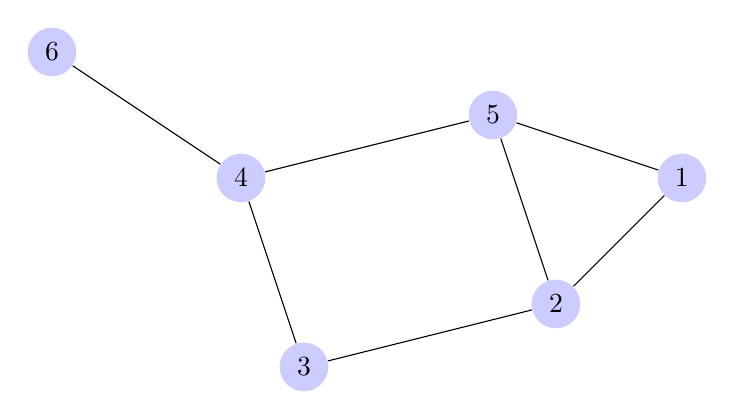
\begin{tikzpicture}
  [scale=.8,auto=left,every node/.style={circle,fill=blue!20}]
  \node (n6) at (1,10) {6};
  \node (n4) at (4,8)  {4};
  \node (n5) at (8,9)  {5};
  \node (n1) at (11,8) {1};
  \node (n2) at (9,6)  {2};
  \node (n3) at (5,5)  {3};

  \foreach \from/\to in {n6/n4, n4/n5,n5/n1,n1/n2,n2/n5,n2/n3,n3/n4}
    \draw (\from) -- (\to);

\end{tikzpicture}
\end{center}

In an undirected graph, we do not distinguish the direction of the edge.  That is, for two vertices $i,j \in V$, we can equivalently write $(i,j)$ or $(j,i)$ to represent the edge.




Alternatively, we will want to consider directed graphs.  We denote these as $G = (V,\mathcal A)$ where $\mathcal A$ is a set of arcs where an arc is a directed edge.

For example, the following directed graph $G$ can be described by the vertex set $V = \{1,2,3,4,5,6\}$ and the edge set $\mathcal A= \{(4,6),(6,4), (4,5), (5,1) (1,2), (2,5), (2,3), (3,4)\}$. 
\begin{center}
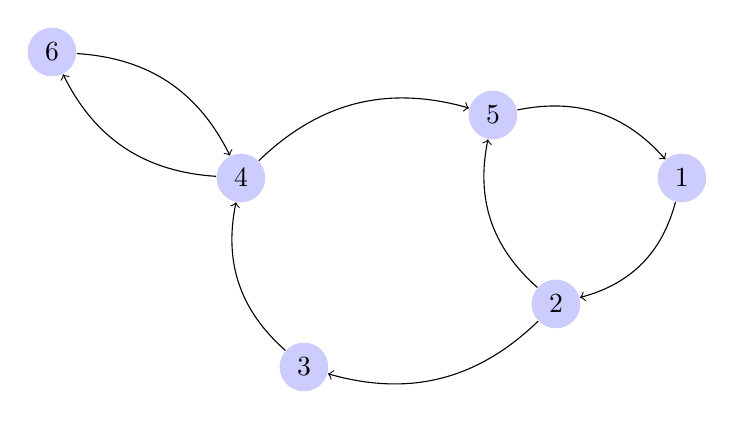
\begin{tikzpicture}
  [scale=.8,auto=left,every node/.style={circle,fill=blue!20}]
  \node (n6) at (1,10) {6};
  \node (n4) at (4,8)  {4};
  \node (n5) at (8,9)  {5};
  \node (n1) at (11,8) {1};
  \node (n2) at (9,6)  {2};
  \node (n3) at (5,5)  {3};

  \foreach \from/\to in {n6/n4,n4/n6,n4/n5,n5/n1,n1/n2,n2/n5,n2/n3,n3/n4}
  	\path[every node/.style={font=\sffamily\small}]
    	(\from) edge[->, bend left] node [left] {} (\to);
   % \draw[->] (\from) to [out=15,in=-15] (\to);

\end{tikzpicture}
\end{center}





\paragraph{Sets}
A finite network $G$ is described by a finite set of vertices $V$ and a finite set $\mathcal{A}$ of arcs. Each arc $(i,j)$ has two key attributes, namely its tail $j \in V$ and its head $i \in V$. 


We think of a (single) commodity as being allowed to "flow" along each arc, from its tail to its head. 
\paragraph{Variables}
Indeed, we have "flow" variables
$$
x_{ij}:=\text { amount of flow on } \operatorname{arc} (i,j) \text{ from vertex $i$ to vertex $j$},
$$
for all $(i,j) \in \mathcal{A}$. 



\subsubsection{Maximum Flow Problem}

\begin{tcolorbox}
\begin{align}
\max \ \ & \sum_{(s, i) \in \mathcal{A}} x_{si} &
\text{max total flow from source}\\
s.t.\ \ 
&\sum_{i : (i,v) \in \mathcal A} x_{i v}-\sum_{j : (v,j) \in \mathcal{A}} x_{v j} =0  &  v \in V \backslash\{s, t\}\\
%[a constraint per edge and a constraint per nonterminal node]\\
&0 \leq x_{ij} \leq  u_{ij} \quad \forall(i,j) \in \mathcal{A}
\end{align}

\end{tcolorbox}
%\documentclass[border=4mm]{standalone}
%\usepackage{tikz}
%\usetikzlibrary{arrows.meta,positioning}
%\begin{document}

\paragraph{Shortest Path Problem}


\begin{tcolorbox}
$$
\begin{aligned}
& \text { minimize } & \sum_{u \rightarrow v} \ell_{u \rightarrow v} \cdot x_{u \rightarrow v} & \\
\text { subject to } & \sum_{u} x_{u \rightarrow s}-\sum_{w} x_{s \rightarrow w} &=1 & \\
\sum_{u} x_{u \rightarrow t}-\sum_{w} x_{t \rightarrow w} &=-1 & \\
\sum_{u} x_{u \rightarrow v}-\sum_{w} x_{v \rightarrow w} &=0 & \text { for every vertex } v \neq s, t \\
x_{u \rightarrow v} & \geq 0 & \text { for every edge } u \rightarrow v
\end{aligned}
$$
\end{tcolorbox}
\begin{example}{Max flow example}{}
\begin{center}
    \begin{tikzpicture}[
      mycircle/.style={
         circle,
         draw=black,
         fill=gray,
         fill opacity = 0.3,
         text opacity=1,
         inner sep=0pt,
         minimum size=20pt,
         font=\small},
         startcircle/.style={
         circle,
         draw=black,
         fill=green,
         fill opacity = 0.3,
         text opacity=1,
         inner sep=0pt,
         minimum size=20pt,
         font=\small},
         endcircle/.style={
         circle,
         draw=black,
         fill=red,
         fill opacity = 0.3,
         text opacity=1,
         inner sep=0pt,
         minimum size=20pt,
         font=\small},
      myarrow/.style={-Stealth},
      node distance=0.6cm and 1.2cm
      ]
      \node[startcircle] (c1) {$s$};
      \node[mycircle,below right=of c1] (c2) {$v_2$};
      \node[mycircle,right=of c2] (c3) {$v_4$};
      \node[mycircle,above right=of c1] (c4) {$v_1$};
      \node[mycircle,right=of c4] (c5) {$v_3$};
      \node[endcircle,below right=of c5] (c6) {$t$};

    \foreach \i/\j/\txt/\p in {% start node/end node/text/position
      c1/c2/8/below,
      c1/c4/11/above,
      c2/c3/11/below,
      c3/c6/4/below,
      c4/c5/12/above,
      c5/c6/15/above,
      c5/c2/4/below,
      c3/c5/7/below,
      c2.70/c4.290/1/below}
       \draw [myarrow] (\i) -- node[sloped,font=\small,\p] {\txt} (\j);


     % draw this outside loop to get proper orientation of 10
     \draw [myarrow] (c4.250) -- node[sloped,font=\small,above,rotate=180] {10} (c2.110);
    \end{tikzpicture}
%\end{document}
\end{center}
\end{example}

\begin{example}{Min Cost Network Flow}{}
\begin{center}
    \begin{tikzpicture}[
      mycircle/.style={
         circle,
         draw=black,
         fill=gray,
         fill opacity = 0.3,
         text opacity=1,
         inner sep=0pt,
         minimum size=20pt,
         font=\small},
         startcircle/.style={
         circle,
         draw=black,
         fill=green,
         fill opacity = 0.3,
         text opacity=1,
         inner sep=0pt,
         minimum size=20pt,
         font=\small},
         endcircle/.style={
         circle,
         draw=black,
         fill=red,
         fill opacity = 0.3,
         text opacity=1,
         inner sep=0pt,
         minimum size=20pt,
         font=\small},
      myarrow/.style={-Stealth},
      node distance=0.6cm and 1.2cm
      ]
      \node[mycircle, label = {left: {\color{blue}-2}}] (c1) {$v_5$};
      \node[mycircle,below right=of c1, label = {below: {\color{blue}-5}}] (c2) {$v_2$};
      \node[mycircle,right=of c2,label = {below: {\color{blue}-6}}] (c3) {$v_4$};
      \node[mycircle,above right=of c1, label = {above: {\color{blue}6}}] (c4) {$v_1$};
      \node[mycircle,right=of c4, label = {above: {\color{blue}-3}}] (c5) {$v_3$};
      \node[mycircle,below right=of c5, label = {right: {\color{blue}10}}] (c6) {$v_6$};
      

    \foreach \i/\j/\txt/\txtr/\p in {% start node/end node/text/position
      c1/c2/8/7/below,
      c1/c4/11/4/above,
      c2/c3/11/7/below,
      c3/c6/4/2/below,
      c4/c5/12/9/above,
      c5/c6/15/2/above,
      c5/c2/4/1/below,
      c3/c5/7/8/below,
      c2.70/c4.290/1/2/below}
       \draw [myarrow] (\i) -- node[sloped,font=\small,\p] {\txt, {\color{red} \txtr}} (\j);

%    \foreach \i/\txt/\p in {% start node/end node/text/position
%      c1/8/left,
%      c2/11/above,
%      c3/2/below,
%      c4/9/above,
%      c5/2/above,
%      c6/1/below}
%       \node[\p] (\i) {\txt};

     % draw this outside loop to get proper orientation of 10
     \draw [myarrow] (c4.250) -- node[sloped,font=\small,above,rotate=180] {10, {\color{red} 1}} (c2.110);
    \end{tikzpicture}
   \end{center}
   \end{example}

\includefigurestatic[][scale = 0.5][h]{network-flow}


\includefigurestatic[][scale = 0.5][h]{network-flow-solution}



\subsubsection{Minimum Cost Network Flow}
\paragraph{Parameters}

We assume that flow on arc $(i,j)$ should be non-negative and should not exceed
$$
u_{ij}:=\text { the flow upper bound on } \operatorname{arc} (i,j) \text {, }
$$
for $(i,j) \in \mathcal{A}$. Associated with each arc $(i,j)$ is a cost
$$
c_{ij}:=\text { cost per-unit-flow on arc } (i,j),
$$
for $(i,j) \in \mathcal{A}$. The (total) cost of the flow $x$ is defined to be
$$
\sum_{(i,j) \in \mathcal{A}} c_{ij} x_{ij} .
$$

We assume that we have further data for the nodes. Namely,
$$
b_{v}:=\text { the net supply at node } v,
$$
for $v \in V$. 

A flow is conservative if the net flow out of node $v$, minus the net flow into node $v$, is equal to the net supply at node $v$, for all nodes $v \in V$.

The (single-commodity min-cost) network-flow problem is to find a minimumcost conservative flow that is non-negative and respects the flow upper bounds on the arcs. 





\paragraph{Objective and Constraints}
We can formulate this as follows:
\begin{tcolorbox}
$$
\begin{aligned}
\min & \sum_{(i,j) \in \mathcal{A}} c_{ij}\, x_{ij} & \text{ minimize cost}\\
& \sum_{(i,v) \in \mathcal{A}} x_{iv}-\sum_{(v,i)  \in \mathcal{A} } x_{vi}=b_{v}, \quad \text{ for all }  v \in V,  & \text{ flow conservation}\\
& 0 \leq x_{ij} \leq u_{ij}, \quad \text{ for all }  (i,j) \in \mathcal{A} .
\end{aligned}
$$
\end{tcolorbox}

\begin{theorem}{Integrality of Network Flow}{integralitynetworkflow}
If the capacities and demands are all integer values, then there always exists an optimal solution to the LP that has integer values.
\end{theorem}

\subsection{Multi-Commodity Network Flow}
In the same vein as the Network Flow Problem
\begin{align*}
\min~& \sum_{k=1}^{K} \sum_{e \in \mathcal{A}} c^k_e x^k_e \\
&\sum_{e\in \mathcal{A} ~:~ t(e)=v} x^k_e - \sum_{e\in \mathcal{A} ~:~ h(e)=v} x^k_e 
= b^k_v,~ \mbox{ for } v \in \mathcal{N},~ k=1,2,\ldots,K;\\
& \sum_{k=0}^{K}  x^k_{e} \leq u_e,~ \mbox{ for } e \in \mathcal{A};\\
&  x^k_{e}\geq 0,~ \mbox{ for } e \in \mathcal{A},~ k=1,2,\ldots,K\\
\end{align*}

Notes:

K=1 is ordinary single-commodity network flow. Integer solutions for free when node-supplies and arc capacities are integer.
K=2 example below with integer data gives a fractional basic optimum. This example doesn't have any feasible integer flow at all.

\begin{remark}{}{}
Unfortunately, the same integrality theorem does not hold in the multi-commodity network flow probem.  Nontheless, if the quanties in each flow are very large, then the LP solution will likely be very close to an integer valued solution.
\end{remark}

\section{Modeling Tricks}
\todoSection{ 40\% complete. Goal 80\% completion date: July 20\\
Notes: Only one modeling trick listed here.  Discuss absolute value application and also making a free variable non-negative.}

\subsection{Maximizing a minimum}
When the constraints could be general, we will write $x \in X$ to define general constraints.  For instance, we could have $X = \{ x \in \R^n : Ax \leq b\}$ of $X  = \{ x \in \R^n : Ax \leq b, x \in \Z^n\}$ or many other possibilities.  


Consider the problem 

\begin{align*}
\max   \quad & \min \{x_1, \dots, x_n\}\\
\text{ such that } \quad &  x \in X
\end{align*}
Having the minimum on the inside is inconvenient.  To remove this, we just define a new variable $y$ and enforce that $y \leq x_i$ and then we maximize $y$.  Since we are maximizing $y$, it will take the value of the smallest $x_i$.  Thus, we can recast the problem as

\begin{align*}
\max\quad    & y\\
\text{ such that } \quad  & y \leq x_i \ \text{ for }\  i=1, \dots, n \\
&  x \in X
\end{align*}

\begin{example}{Minimizing an Absolute Value}{}
Note that 
$$
|t| = \max(t, -t),
$$
Thus, if we need to minimize $|t|$ we can instead write

\begin{align}
\min z\\
s.t.\\
t \leq z
-t \leq z
\end{align}

\end{example}

\section{Other examples}


\href{https://gurobi.github.io/modeling-examples/food_manufacturing_1_2/food_manufacture_1.html}{Food manfacturing - GUROBI}

\href{https://www.andrew.cmu.edu/user/gc0v/webpub/book.pdf}{Optimization Methods in Finance - Corneujols, T\"ut\"unc\"u}

\chapter{Graphically Solving Linear Programs}
\todoChapter{ 50\% complete. Goal 80\% completion date: July 20\\
Notes: }
\begin{outcome}
\begin{enumerate}
\item[A.] Learn how to plot the feasible region and the objective function.
\item[B.] Identify and compute extreme points of the feasible region.
\item[C.] Find the optimal solution(s) to a linear program graphically.
\item[D.] Classify the type of result of the problem as infeasible, unbounded, unique optimal solution, or infinitely many optimal solutions.
\end{enumerate}
\end{outcome}

Linear Programs (LP's) with two variables can be solved graphically by plotting the feasible region along with the level curves of the objective function.\footnote{Special thanks to Joshua Emmanual and Christopher Griffin for sharing their content to help put this section together. Proper citations and referenes are forthcoming.} We will show that we can find a point in the feasible region that maximizes the objective function using the level curves of the objective function.

We will begin with an easy example that is bounded and investigate the structure of the feasible region.  We will then explore other examples.
\section{Nonempty and Bounded Problem}
\todoSection{ 20\% complete. Goal 80\% completion date: July 20\\
Notes: Need to work on this section.}
Consider the problem
\begin{align*}
\max \quad & 2 X+5 Y \\
\text { s.t. } \quad 
&X+2 Y \leq 16 \\
&5 X+3 Y \leq  45 \\
&X, Y  \geq 0
\end{align*}

We want to start by plotting the \emph{feasible region}, that is, the set points $(X,Y)$ that satisfy all the constraints. 

We can plot this by first plotting the four lines
\begin{itemize}
\item $X+2 Y = 16$
\item $5 X+3 Y = 45$
\item $X = 0$
\item $Y = 0$
\end{itemize}
and then shading in the side of the space cut out by the corresponding inequality.
\begin{center}
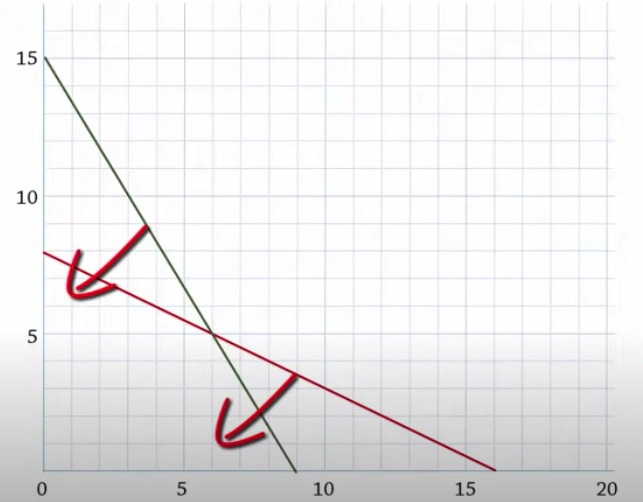
\includegraphics[scale = 0.4]{screenshots/example0-inequalities}
\end{center}

The resulting feasible region can then can be shaded in as the region that satisfies all the inequalties.

\begin{center}
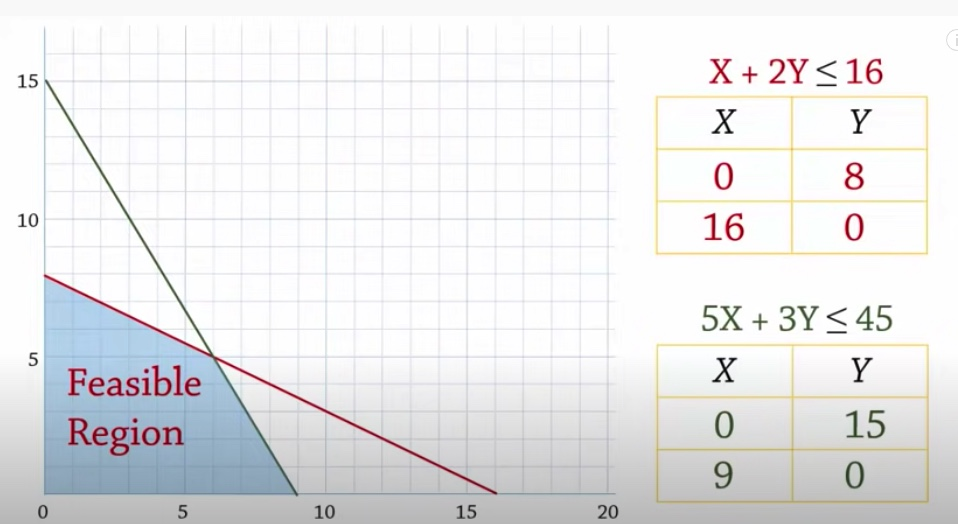
\includegraphics[scale = 0.4]{screenshots/example0-feasible-region}
\end{center}

Notice that the feasible region is nonempty (it has points that satisfy all the inequalities) and also that it is bounded (the feasible points dont continue infinitly in any direction).

We want to identify the \emph{extreme points} (i.e., the corners) of the feasible region. 
Understanding these points will be critical to understanding the optimal solutions of the model.
Notice that all extreme points can be computed by finding the intersection of 2 of the lines.   But!  Not all intersections of any two lines are feasible.  

We will later use the terminology \emph{basic feasible solution} for an extreme point of the feasible region, and \emph{basic solution} as a point that is the intersection of 2 lines, but is actually infeasible (does not satisfy all the constraints).

\begin{center}
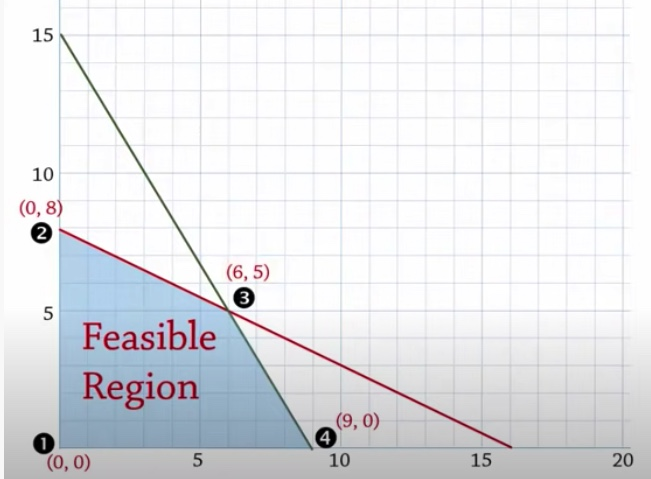
\includegraphics[scale = 0.4]{screenshots/example0-extreme-points}
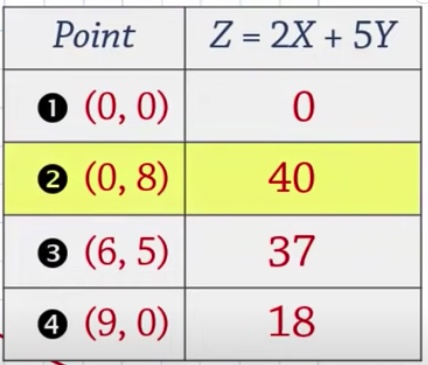
\includegraphics[scale = 0.4]{screenshots/example0-extreme-point-solutions}
\end{center}

\begin{theorem}{Optimal Extreme Point}{optimalextremepoint}
If the feasible region is nonempty and bounded, then there exists an optimal solution at an extreme point of the feasible region.
\end{theorem}

We will explore why this theorem is true, and also what happens when the feasible region does not satisfy the assumtions of either nonempty or bounded.
We illustrate the idea first using the problem from Example \ref{ex:ToyMaker}.

\begin{figure}[H] 
\centering
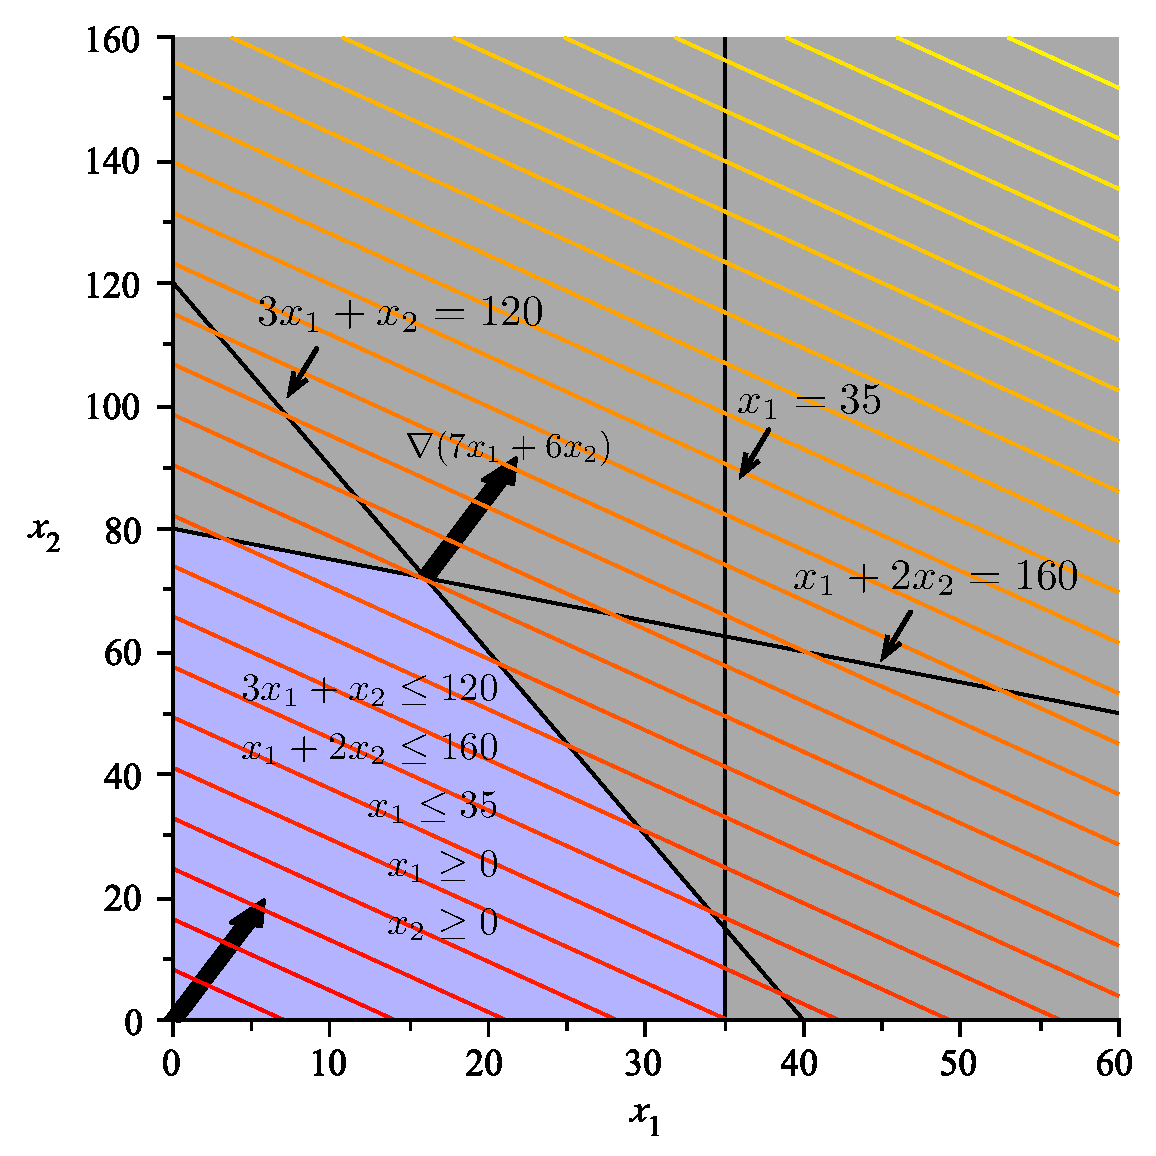
\includegraphics[scale=0.4]{FeasibleRegion.pdf}
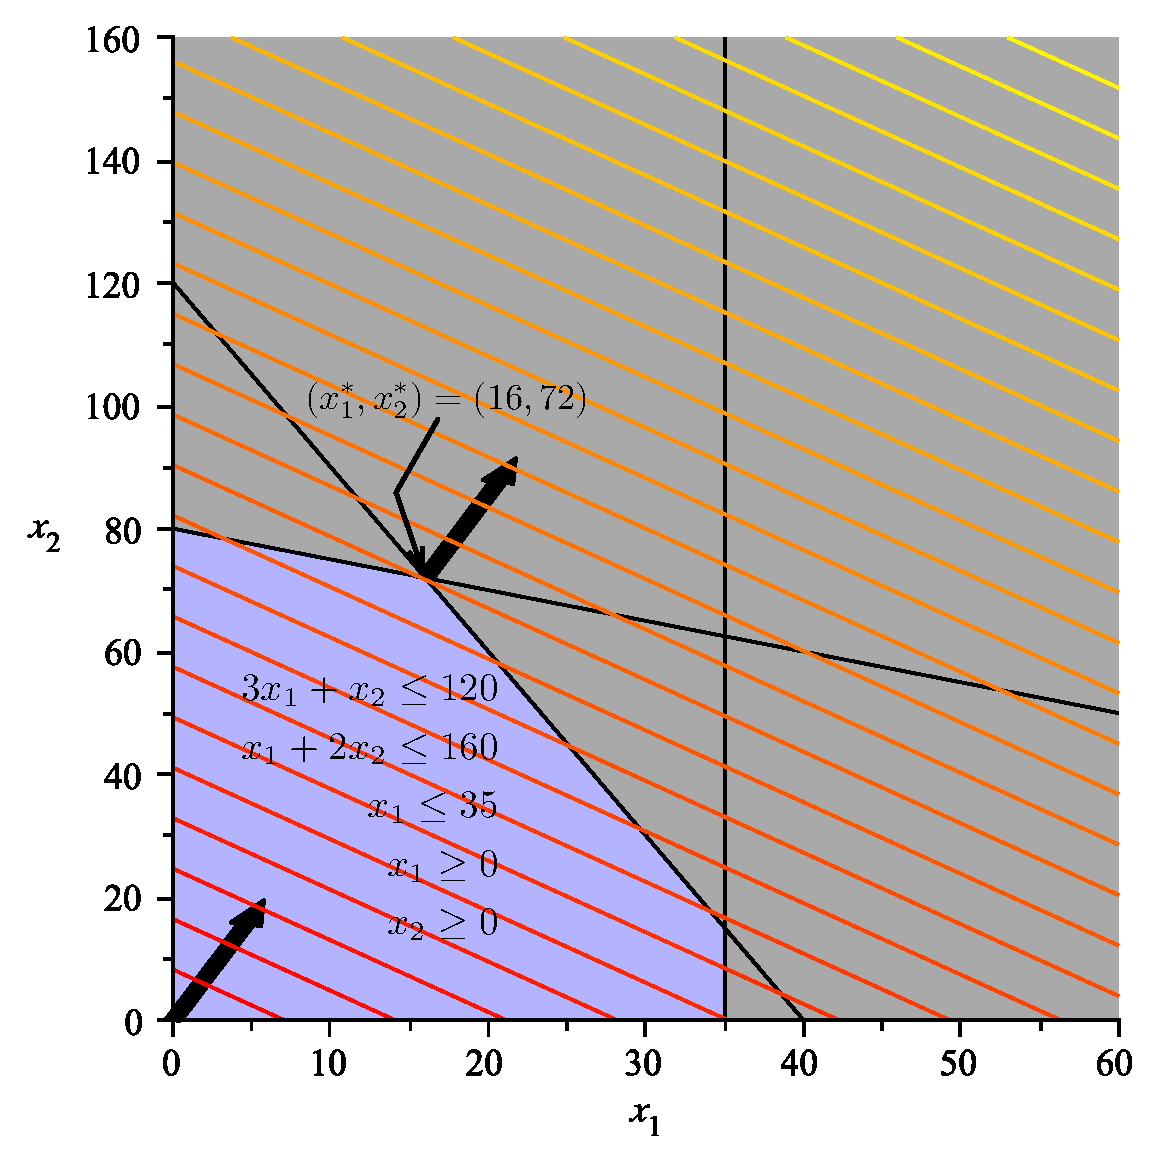
\includegraphics[scale=0.4]{FeasibleRegionWithMax.pdf}
\caption{Feasible Region and Level Curves of the Objective Function: The shaded region in the plot is the feasible region and represents the intersection of the five inequalities constraining the values of $x_1$ and $x_2$. On the right, we see the optimal solution is the ``last'' point in the feasible region that intersects a level set as we move in the direction of increasing profit.}
\label{fig:ToyExampleFeasibleRegion}
\end{figure}

\begin{example}{Continuation of Example \ref{ex:ToyMaker}}{}Let's continue the example of the Toy Maker begin in Example \ref{ex:ToyMaker}.  Solve this problem graphically.
\end{example}
\begin{solution} To solve the linear programming problem graphically, begin by drawing the feasible region. This is shown in the blue shaded region of Figure \ref{fig:ToyExampleFeasibleRegion}. 


After plotting the feasible region, the next step is to plot the level curves of the objective function. In our problem, the level sets will have the form:
\begin{displaymath}
7x_1 + 6x_2 = c \implies x_2 = \frac{-7}{6}x_1 + \frac{c}{6}
\end{displaymath}
This is a set of parallel lines with slope $-7/6$ and intercept $c/6$ where $c$ can be varied as needed. The level curves for various values of $c$ are parallel lines. In Figure \ref{fig:ToyExampleFeasibleRegion} they are shown in colors ranging from red to yellow depending upon the value of $c$. Larger values of $c$ are more yellow. 

To solve the linear programming problem, follow the level sets along the gradient (shown as the black arrow) until the last level set (line) intersects the feasible region. If you are doing this by hand, you can draw a single line of the form $7x_1 + 6x_2 = c$ and then simply draw parallel lines in the direction of the gradient $(7,6)$. At some point, these lines will fail to intersect the feasible region. The last line to intersect the feasible region will do so at a point that maximizes the profit. In this case, the point that maximizes $z(x_1,x_2) = 7x_1 + 6x_2$, subject to the constraints given, is $(x_1^*, x_2^*) = (16,72)$. 
\newpage
Note the point of optimality $(x_1^*, x_2^*) = (16,72)$ is at a corner of the feasible region. This corner is formed by the intersection of the two lines: $3x_1 + x_2 = 120$ and $x_1 + 2x_2 = 160$. In this case, the constraints 
\begin{gather*}
3x_1 + x_2 \leq 120\\
x_1 + 2x_2 \leq 160
\end{gather*}
are both \textit{binding}, while the other constraints are non-binding. In general, we will see that when an optimal solution to a linear programming problem exists, it will always be at the intersection of several binding constraints; that is, it will occur at a corner of a higher-dimensional polyhedron.  
\end{solution}

We can now define an algorithm for identifying the solution to a linear programing problem in two variables with a \textit{bounded} feasible region (see Algorithm \ref{alg:GraphLPBoundedUniqueSoln}): 
\begin{algorithm}
\caption{Algorithm for Solving a Two Variable Linear Programming Problem Graphically--Bounded Feasible Region, Unique Solution Case}
\label{alg:GraphLPBoundedUniqueSoln}
\begin{center}
\begin{minipage}[t]{\textwidth-1em}
\underline{\textbf{Algorithm for Solving a Linear Programming Problem Graphically}}\\
\textit{Bounded Feasible Region, Unique Solution}
\begin{enumerate*}
\item Plot the feasible region defined by the constraints.
\item Plot the level sets of the objective function.
\item For a maximization problem, identify the level set corresponding the greatest (least, for minimization) objective function value that intersects the feasible region. This point will be at a corner. 
\item The point on the corner intersecting the greatest (least) level set is a solution to the linear programming problem.  
\end{enumerate*}
\end{minipage}
\end{center}
\end{algorithm}

The example linear programming problem presented in the previous section has a single optimal solution. In general, the following outcomes can occur in solving a linear programming problem: 
\begin{enumerate*}
\item The linear programming problem has a unique solution. (We've already seen this.)
\item There are infinitely many alternative optimal solutions.
\item There is no solution and the problem's objective function can grow to positive infinity for maximization problems (or negative infinity for minimization problems). 
\item There is no solution to the problem at all. 
\end{enumerate*}

Case 3 above can only occur when the feasible region is unbounded; that is, it cannot be surrounded by a ball with finite radius. We will illustrate each of these possible outcomes in the next four sections. We will prove that this is true in a later chapter.



\section{Infinitely Many Optimal Solutions}
\todoSection{ 20\% complete. Goal 80\% completion date: July 20\\
Notes: Need to work on this section.}
It can happen that there is more than one solution.  In fact, in this case, there are infinitly many optimal solutions.  
We'll study a specific linear programming problem with an infinite number of solutions by modifying the objective function in Example \ref{ex:ToyMaker}. 
\begin{example}{Toy Maker Alternative Solutions}{ex:ToyMakerAltOptSoln}
Suppose the toy maker in Example \ref{ex:ToyMaker} finds that it can sell planes for a profit of $\$18$ each instead of $\$7$ each. The new linear programming problem becomes:
\begin{equation}
\left\{
\begin{aligned}
\max\;\;& z(x_1,x_2) = 18x_1 + 6x_2\\
s.t.\;\;&  3x_1 + x_2 \leq 120\\
& x_1 + 2x_2 \leq 160\\
& x_1 \leq 35\\
& x_1 \geq 0\\
& x_2 \geq 0
\end{aligned}
\right.
\label{eqn:ToyMakerAltOptSoln}
\end{equation}
\end{example}

\begin{solution}
Applying our graphical method for finding optimal solutions to linear programming problems yields the plot shown in Figure \ref{fig:ToyMakerAltOptSoln}. The level curves for the function $z(x_1,x_2) = 18x_1 + 6x_2$ are \textit{parallel} to one face of the polygon boundary of the feasible region. Hence, as we move further up and to the right in the direction of the gradient (corresponding to larger and larger values of $z(x_1, x_2)$) we see that there is not \textit{one} point on the boundary of the feasible region that intersects that level set with greatest value, but instead a side of the polygon boundary described by the line $3x_1 + x_2 = 120$ where $x_1 \in [16, 35]$. Let:
\begin{displaymath}
S = \{(x_1,x_2) | 3x_1 + x_2 \leq 120,\,x_1 + 2x_2 \leq 160,\,x_1 \leq 35,\,x_1,x_2 \geq 0\}
\end{displaymath} 
that is, $S$ is the feasible region of the problem. Then for any value of $x_1^* \in [16,35]$ and any value $x_2^*$ so that  $3x_1^* + x_2^* = 120$, we will have $z(x_1^*, x_2^*) \geq z(x_1, x_2)$ for all $(x_1,x_2) \in S$. Since there are infinitely many values that $x_1$ and $x_2$  may take on, we see this problem has an infinite number of alternative optimal solutions.
\begin{figure}[H]
\centering
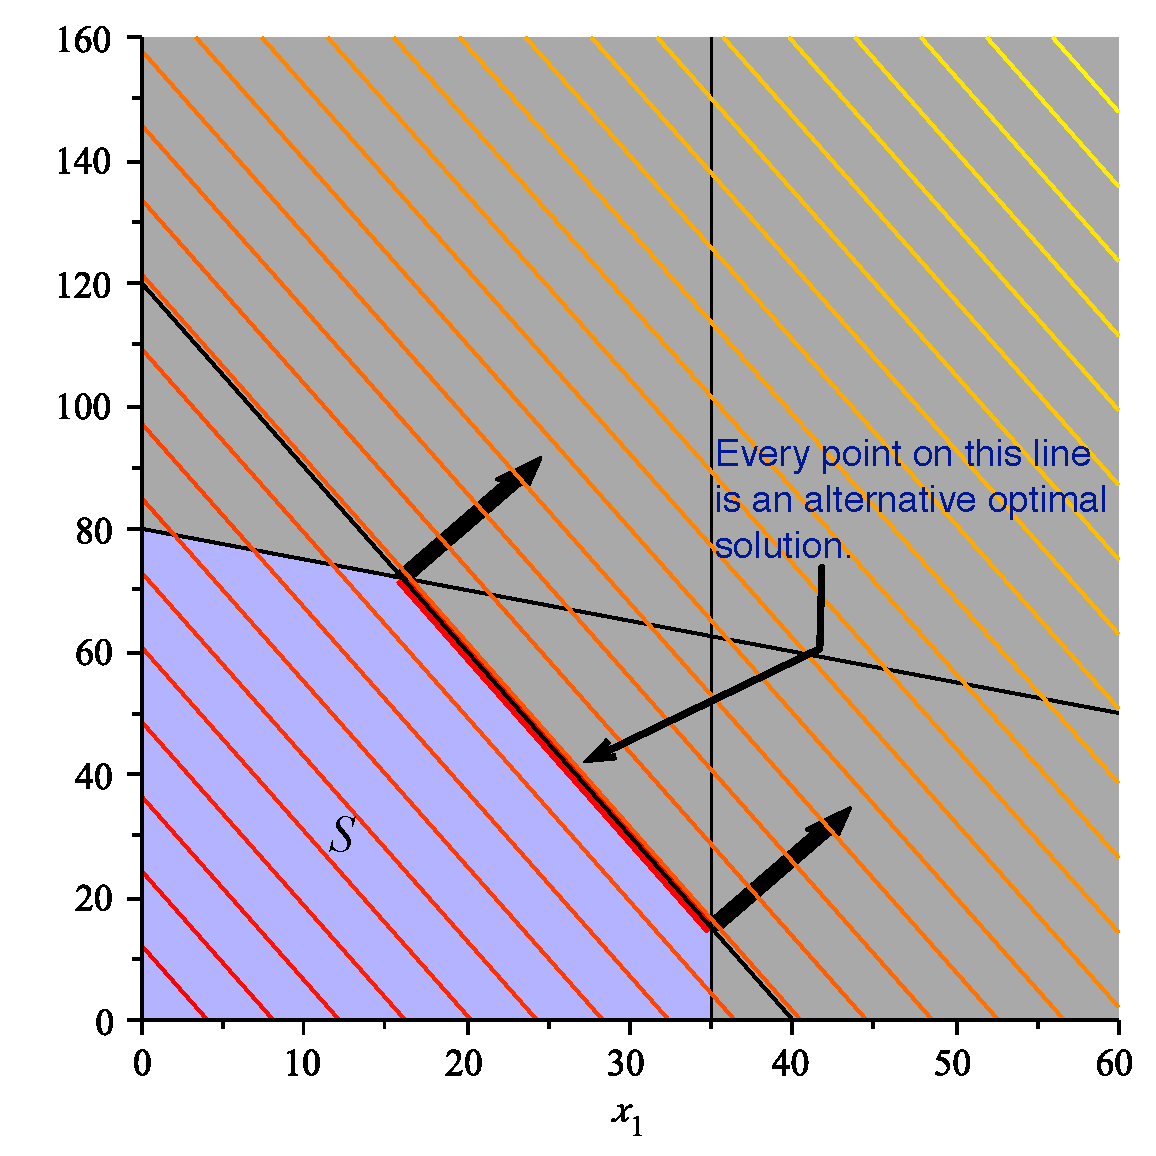
\includegraphics[scale=0.4]{AltOptSolns.pdf}
\caption{An example of infinitely many alternative optimal solutions in a linear programming problem. The level curves for $z(x_1,x_2) = 18x_1 + 6x_2$ are \textit{parallel} to one face of the polygon boundary of the feasible region. Moreover, this side contains the points of greatest value for $z(x_1,x_2)$ inside the feasible region. Any combination of $(x_1,x_2)$ on the line $3x_1 + x_2 = 120$ for $x_1 \in [16, 35]$ will provide the largest possible value $z(x_1,x_2)$ can take in the feasible region $S$.}
\label{fig:ToyMakerAltOptSoln}
\end{figure}
%\label{ex:ToyMakerAltOptSoln}
\end{solution}






\begin{exercise}{}{} Use the graphical method for solving linear programming problems to solve the linear programming problem you defined in Exercise \ref{exer:ChemicalPlant}.
\end{exercise}



Based on the example in this section, we can modify our algorithm for finding the solution to a linear programming problem graphically to deal with situations with an infinite set of alternative optimal solutions (see Algorithm \ref{alg:GraphLPBounded}):
\begin{algorithm}[H]
\caption{Algorithm for Solving a Two Variable Linear Programming Problem Graphically--Bounded Feasible Region Case}
\label{alg:GraphLPBounded}
\begin{center}
\begin{minipage}[t]{\textwidth-1em}
\underline{\textbf{Algorithm for Solving a Linear Programming Problem Graphically}}\\
\textit{Bounded Feasible Region}
\begin{enumerate*}
\item Plot the feasible region defined by the constraints.
\item Plot the level sets of the objective function.
\item For a maximization problem, identify the level set corresponding the greatest (least, for minimization) objective function value that intersects the feasible region. This point will be at a corner. 
\item The point on the corner intersecting the greatest (least) level set is a solution to the linear programming problem. 
\item \textbf{If the level set corresponding to the greatest (least) objective function value is parallel to a side of the polygon boundary next to the corner identified, then there are infinitely many alternative optimal solutions and any point on this side may be chosen as an optimal solution.} 
\end{enumerate*}
\end{minipage}
\end{center}
\end{algorithm}

\begin{exercise}{}{} Modify the linear programming problem from Exercise \ref{exer:ChemicalPlant} to obtain a linear programming problem with an infinite number of alternative optimal solutions. Solve the new problem and obtain a description for the set of alternative optimal solutions. [Hint: Just as in the example, $x_1$ will be bound between two value corresponding to a side of the polygon. Find those values and the constraint that is binding. This will provide you with a description of the form for any $x_1^* \in [a,b]$ and $x_2^*$ is chosen so that $cx_1^* + dx_2^* = v$, the point $(x_1^*, x_2^*)$ is an alternative optimal solution to the problem. Now you fill in values for $a$, $b$, $c$, $d$ and $v$.]
\end{exercise}

\section{Problems with No Solution} 
\todoSection{ 20\% complete. Goal 80\% completion date: July 20\\
Notes: Need to work on this section.}
Recall for \textit{any} mathematical programming problem, the feasible set or region is simply a subset of $\mathbb{R}^n$. If this region is empty, then there is no solution to the mathematical programming problem and the problem is said to be \textit{over constrained}. In this case, we say that the problem is \emph{infeasible}.  We illustrate this case for linear programming problems with the following example.
\begin{example}{Infeasible Problem}
 Consider the following linear programming problem:
\begin{equation}
\left\{
\begin{aligned}
\max\;\;& z(x_1,x_2) = 3x_1 + 2x_2\\
s.t.\;\;&  \frac{1}{40}x_1 + \frac{1}{60}x_2 \leq 1\\
& \frac{1}{50}x_1 + \frac{1}{50}x_2 \leq 1\\
& x_1 \geq 30\\
& x_2 \geq 20
\end{aligned}
\right.
\label{eqn:LPInfeasible}
\end{equation}
\end{example}
\begin{solution}
The level sets of the objective and the constraints are shown in Figure \ref{fig:LPInfeasible}. 
\begin{figure}[H]
\centering
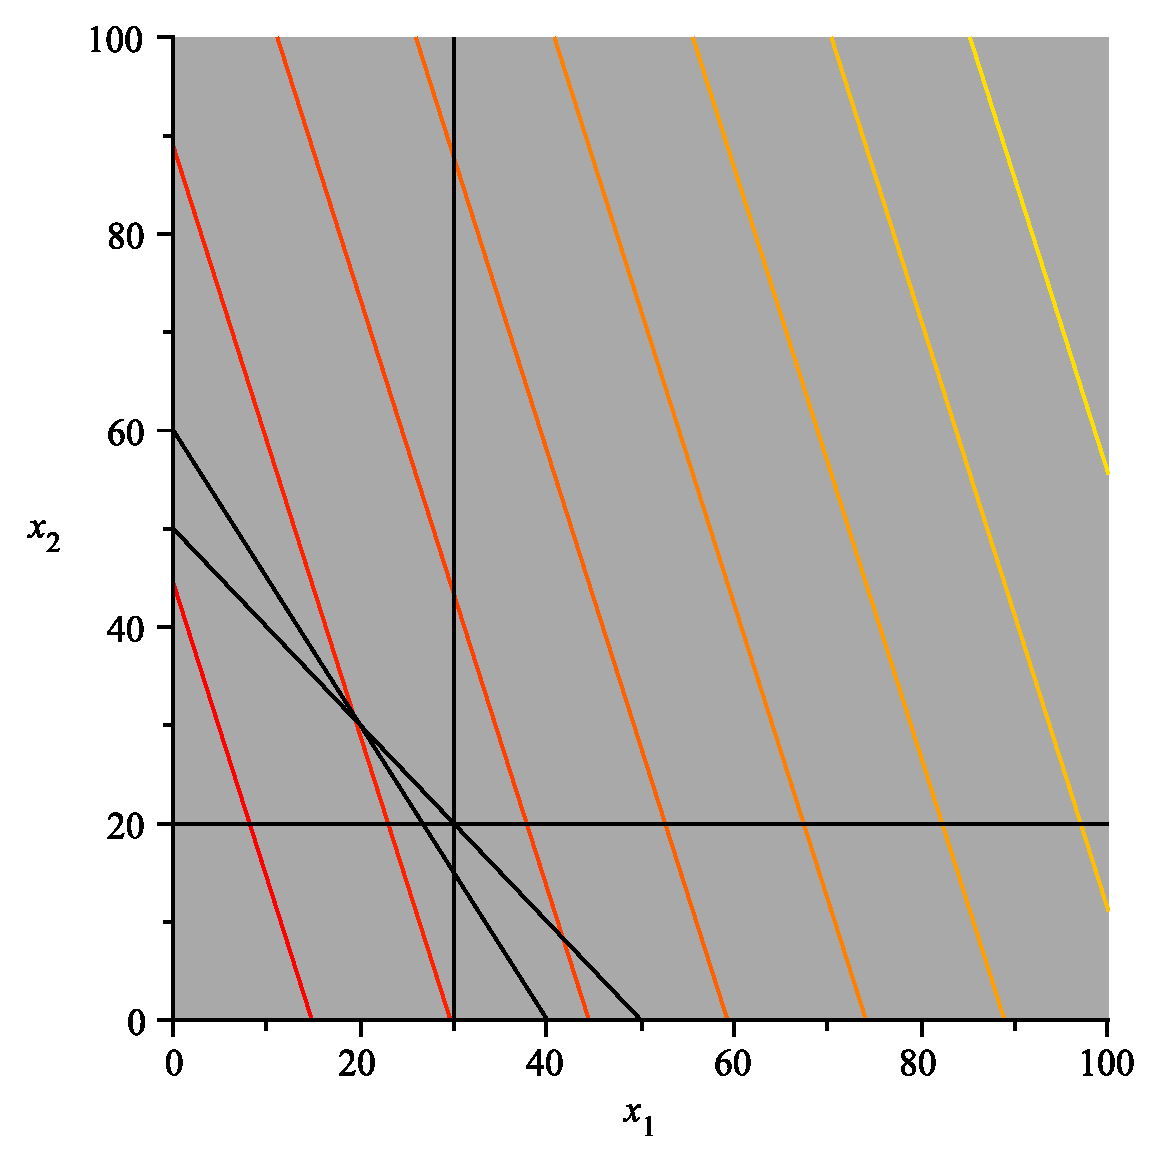
\includegraphics[scale=0.4]{LPNoSoln.pdf}
\caption{A Linear Programming Problem with no solution. The feasible region of the linear programming problem is empty; that is, there are no values for $x_1$ and $x_2$ that can simultaneously satisfy all the constraints. Thus, no solution exists.}
\label{fig:LPInfeasible}
\end{figure}

The fact that the feasible region is empty is shown by the fact that in Figure \ref{fig:LPInfeasible} there is no blue region--i.e., all the regions are gray indicating that the constraints are not satisfiable.
\label{ex:LPNoSoln}
\end{solution} 
Based on this example, we can modify our previous algorithm for finding the solution to linear programming problems graphically (see Algorithm \ref{alg:GraphLPBoundedEmpty}):
\begin{algorithm}[H]
\caption{Algorithm for Solving a Two Variable Linear Programming Problem Graphically--Bounded Feasible Region Case}
\label{alg:GraphLPBoundedEmpty}
\begin{center}
\begin{minipage}[t]{\textwidth-1em}
\underline{\textbf{Algorithm for Solving a Linear Programming Problem Graphically}}\\
\textit{Bounded Feasible Region}
\begin{enumerate*}
\item Plot the feasible region defined by the constraints.
\item \textbf{If the feasible region is empty, then no solution exists.}
\item Plot the level sets of the objective function.
\item For a maximization problem, identify the level set corresponding the greatest (least, for minimization) objective function value that intersects the feasible region. This point will be at a corner. 
\item The point on the corner intersecting the greatest (least) level set is a solution to the linear programming problem. 
\item \textbf{If the level set corresponding to the greatest (least) objective function value is parallel to a side of the polygon boundary next to the corner identified, then there are infinitely many alternative optimal solutions and any point on this side may be chosen as an optimal solution.} 
\end{enumerate*}
\end{minipage}
\end{center}
\end{algorithm}

\section{Problems with Unbounded Feasible Regions}
\todoSection{ 20\% complete. Goal 80\% completion date: July 20\\
Notes: Need to work on this section.}
Consider the problem

\begin{align*}
\min \quad & Z =5 X+7 Y  \\ 
\text { s.t. } \quad & X+3 Y \geq 6 \\ 
&5 X+ 2 Y \geq 10 \\ 
&Y  \leq 4 \\ 
&X, Y  \geq 0 
\end{align*}

\begin{center}
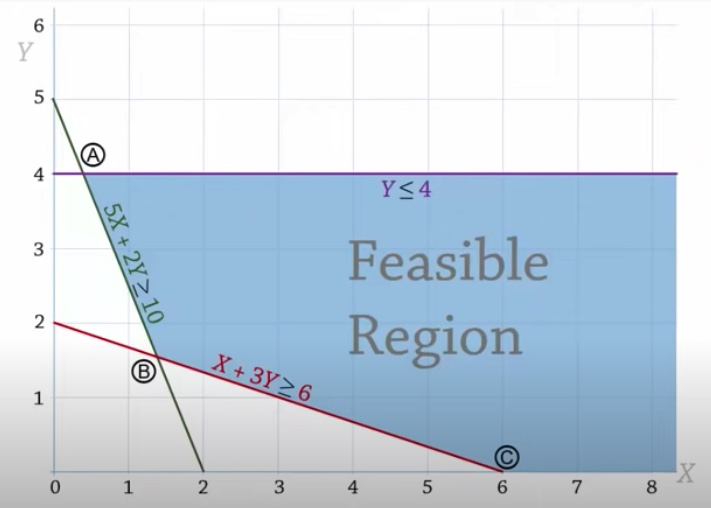
\includegraphics[scale = 0.4]{screenshots/example1-feasible-region}
\end{center}

As you can see, the feasible region is \emph{unbounded}.  In particular, from any point in the feasible region, one can always find another feasible point by increasing the $X$ coordinate (i.e., move to the right in the picture).   However, this does not necessarily mean that the optimization problem is unbounded.

Indeed, the optimal solution is at the B, the extreme point in the lower left hand corner.

\todo[inline]{To do: add contours to plot to show extreme point is the optimal solution.}

\begin{center}
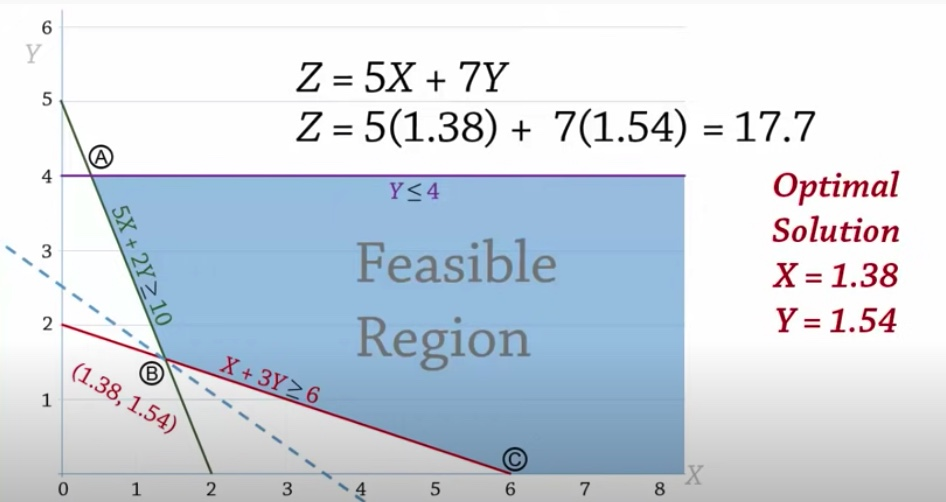
\includegraphics[scale = 0.4]{screenshots/example1-optimal-solution}
\end{center}


Consider however, if we consider a different problem where we try to maximize the objective
\begin{align*}
\max \quad & Z = 5X + 7Y\\ 
\text { s.t. } \quad & X+3 Y \geq 6 \\ 
&5 X+ 2 Y \geq 10 \\ 
&Y  \leq 4 \\ 
&X, Y  \geq 0 
\end{align*}

\begin{solution}
This optimization problem is unbounded!  For example, notice that the point $(X,Y) = (n,0)$ is feasible for all $n=1,2,3,\dots,$.   Then the objective function $Z = 5n + 0$ follows the sequence $5, 10, 15, \dots,$, which diverges to infinity.   
\end{solution}


Again, we'll tackle the issue of linear programming problems with unbounded feasible regions by illustrating the possible outcomes using examples.

\begin{example}{}{} Consider the linear programming problem below:
\begin{equation}
\left\{
\begin{aligned}
\max\;\;& z(x_1,x_2) = 2x_1 - x_2\\
s.t.\;\;& x_1 - x_2 \leq 1\\
& 2x_1 + x_2 \geq 6\\
&x_1,x_2 \geq 0
\end{aligned}
\right.
\label{eqn:LPUnboundFeasibleRegion1}
\end{equation}
\end{example}
\begin{solution}
The feasible region and level curves of the objective function are shown in Figure \ref{fig:LPUnboundFeasibleRegion1}. 
\begin{figure}[H]%[htbp]
\centering
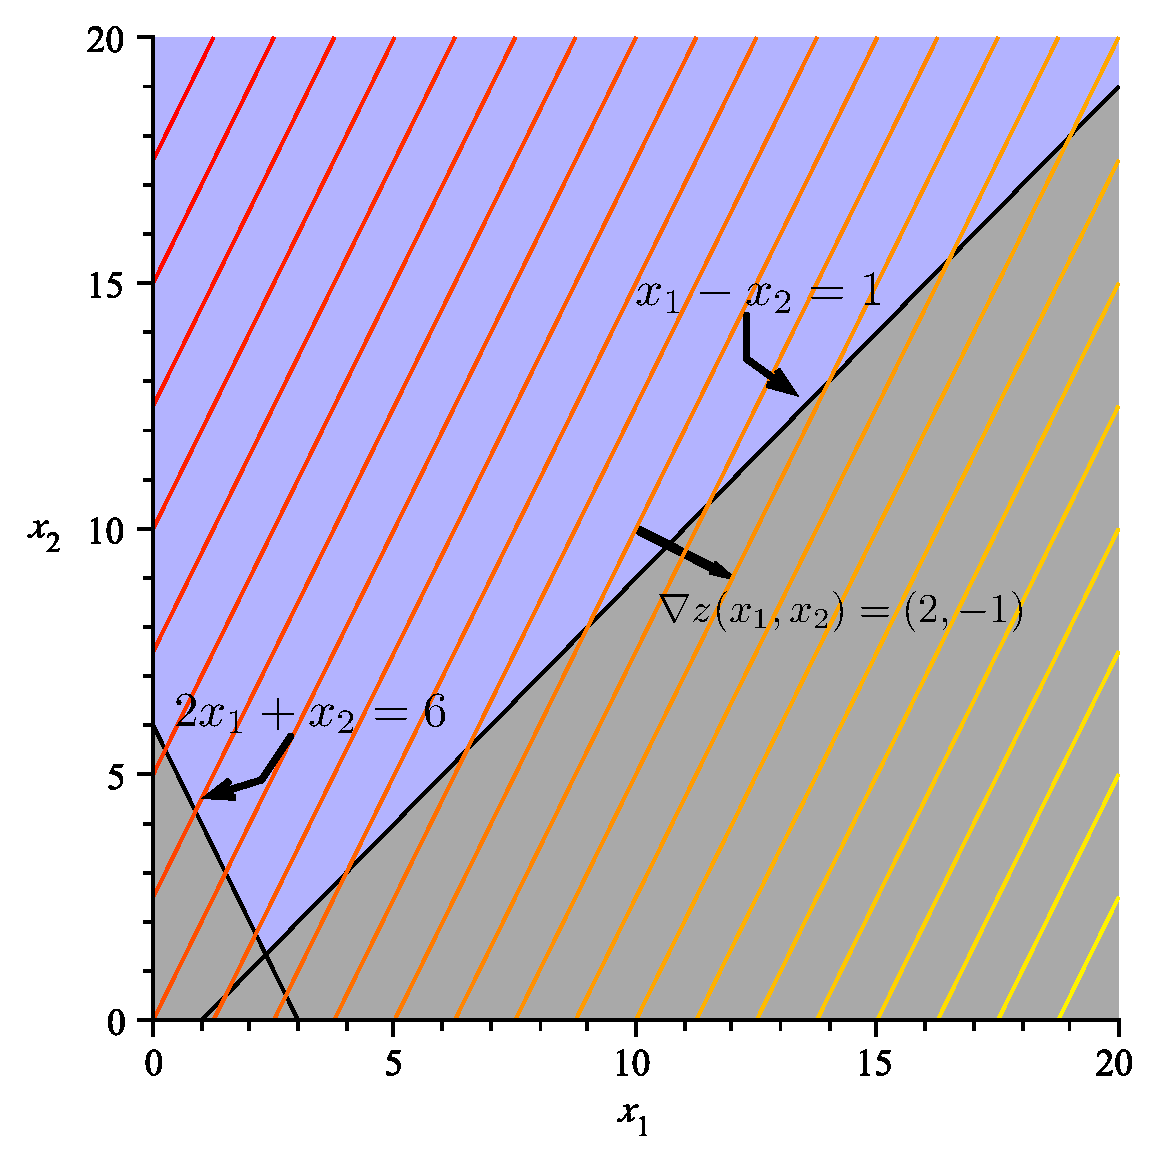
\includegraphics[scale=0.4]{UnboundedFeasibleRegion.pdf}
\caption{A Linear Programming Problem with Unbounded Feasible Region: Note that we can continue to make level curves of $z(x_1,x_2)$ corresponding to larger and larger values as we move down and to the right. These curves will continue to intersect the feasible region for any value of $v = z(x_1,x_2)$ we choose. Thus, we can make $z(x_1,x_2)$ as large as we want and still find a point in the feasible region that will provide this value. Hence, the optimal value of $z(x_1,x_2)$ subject to the constraints $+\infty$. That is, the problem is unbounded.}
\label{fig:LPUnboundFeasibleRegion1}
\end{figure}
The feasible region in Figure \ref{fig:LPUnboundFeasibleRegion1} is clearly unbounded since it stretches upward along the $x_2$ axis infinitely far and also stretches rightward along the $x_1$ axis infinitely far, bounded below by the line $x_1-x_2 = 1$. There is no way to enclose this region by a disk of finite radius, hence the feasible region is not bounded. 

We can draw more level curves of $z(x_1,x_2)$  in the direction of increase (down and to the right) as long as we wish. There will always be an intersection point with the feasible region because it is infinite. That is, these curves will continue to intersect the feasible region for any value of $v = z(x_1,x_2)$ we choose. Thus, we can make $z(x_1,x_2)$ as large as we want and still find a point in the feasible region that will provide this value. Hence, the largest value $z(x_1,x_2)$ can take when $(x_1,x_2)$ are in the feasible region is $+\infty$. That is, the problem is unbounded.
\label{ex:LPUnboundFeasibleRegion1}
\end{solution}

Just because a linear programming problem has an unbounded feasible region does not imply that there is not a finite solution. We illustrate this case by modifying example \ref{ex:LPUnboundFeasibleRegion1}. 

\begin{example}{Continuation of Example \ref{ex:LPUnboundFeasibleRegion1}}{ex:LPUnboundFeasibleRegion2}
Consider the linear programming problem from Example \ref{ex:LPUnboundFeasibleRegion1} with the new objective function: $z(x_1,x_2) = (1/2)x_1 - x_2$. Then we have the new problem:
\begin{equation}
\left\{
\begin{aligned}
\max\;\;& z(x_1,x_2) =\frac{1}{2}x_1 - x_2\\
s.t.\;\;& x_1 - x_2 \leq 1\\
& 2x_1 + x_2 \geq 6\\
&x_1,x_2 \geq 0
\end{aligned}
\right.
\label{eqn:LPUnboundFeasibleRegion2}
\end{equation}
\end{example}
\begin{solution}
The feasible region, level sets of $z(x_1,x_2)$ and gradients are shown in Figure \ref{fig:LPUnboundFeasibleRegion2}. In this case note, that the direction of increase of the objective function is \textit{away} from the direction in which the feasible region is unbounded (i.e., downward). As a result, the point in the feasible region with the largest $z(x_1,x_2)$ value is $(7/3,4/3)$. Again this is a vertex: the binding constraints are $x_1 - x_2 = 1$ and $2x_1 + x_2 = 6$ and the solution occurs at the point these two lines intersect.
\begin{figure}[H]%[htbp]
\centering
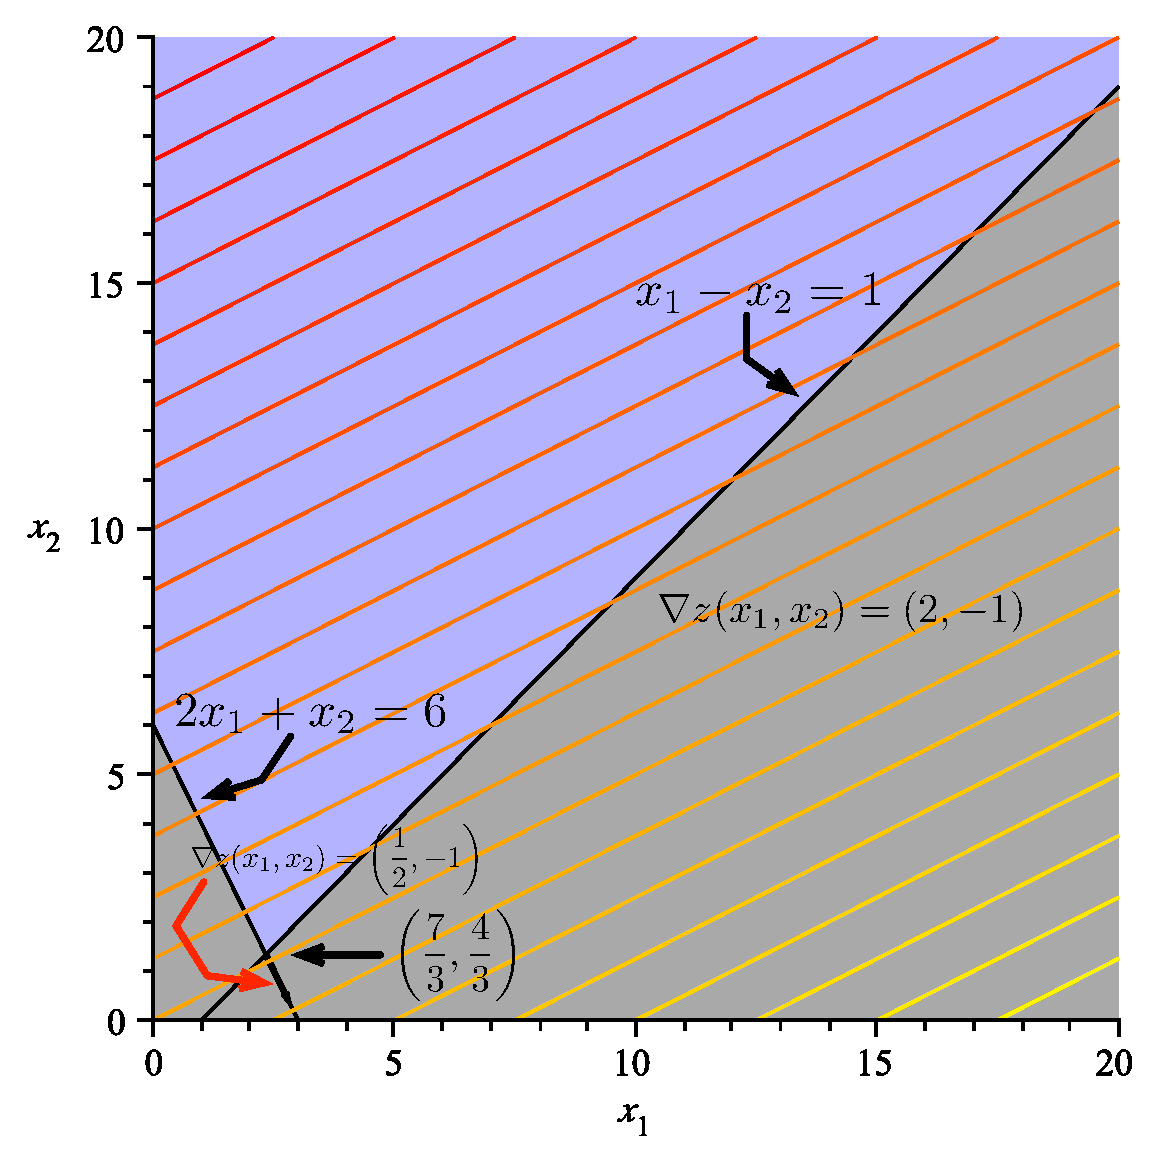
\includegraphics[scale=0.4]{UnboundedFeasibleRegionFiniteSolution.pdf}
\caption{A Linear Programming Problem with Unbounded Feasible Region and Finite Solution: In this problem, the level curves of $z(x_1,x_2)$ increase in a more ``southernly'' direction that in Example \ref{ex:LPUnboundFeasibleRegion2}--that is, \textit{away} from the direction in which the feasible region increases without bound. The point in the feasible region with largest $z(x_1,x_2)$ value is $(7/3,4/3)$. Note again, this is a vertex.}
\label{fig:LPUnboundFeasibleRegion2}
\end{figure}
\label{ex:LPUnboundFeasibleRegion2}
\end{solution}
Based on these two examples, we can modify our algorithm for graphically solving a two variable linear programming problems to deal with the case when the feasible region is unbounded.
\begin{algorithm}
\caption{Algorithm for Solving a Linear Programming Problem Graphically--Bounded and Unbounded Case}
\label{alg:GraphLPAlmostGeneral}
\begin{center}
\begin{minipage}[t]{\textwidth-1em}
\underline{\textbf{Algorithm for Solving a Two Variable Linear Programming Problem Graphically}}
\begin{enumerate*}
\item Plot the feasible region defined by the constraints.
\item If the feasible region is empty, then no solution exists.
\item If the feasible region is unbounded goto Line 8. Otherwise, Goto Line 4.
\item Plot the level sets of the objective function.
\item For a maximization problem, identify the level set corresponding the greatest (least, for minimization) objective function value that intersects the feasible region. This point will be at a corner. 
\item The point on the corner intersecting the greatest (least) level set is a solution to the linear programming problem. 
\item \textbf{If the level set corresponding to the greatest (least) objective function value is parallel to a side of the polygon boundary next to the corner identified, then there are infinitely many alternative optimal solutions and any point on this side may be chosen as an optimal solution.} 
\item (The feasible region is unbounded): Plot the level sets of the objective function.
\item If the level sets intersect the feasible region at larger and larger (smaller and smaller for a minimization problem), then the problem is unbounded and the solution is $+\infty$ ($-\infty$ for minimization problems). 
\item Otherwise, identify the level set corresponding the greatest (least, for minimization) objective function value that intersects the feasible region. This point will be at a corner. 
\item The point on the corner intersecting the greatest (least) level set is a solution to the linear programming problem. 
\textbf{If the level set corresponding to the greatest (least) objective function value is parallel to a side of the polygon boundary next to the corner identified, then there are infinitely many alternative optimal solutions and any point on this side may be chosen as an optimal solution.} 
\end{enumerate*}
\end{minipage}
\end{center}
\end{algorithm}

\begin{exercise}{}{} Does the following problem have a bounded solution? Why?
\begin{equation}
\left\{
\begin{aligned}
\boldsymbol{\min}\;\;& z(x_1,x_2) = 2x_1 - x_2\\
s.t.\;\;& x_1 - x_2 \leq 1\\
& 2x_1 + x_2 \geq 6\\
&x_1,x_2 \geq 0
\end{aligned}
\right.
\end{equation}
[Hint: Use Figure \ref{fig:LPUnboundFeasibleRegion2} and Algorithm \ref{alg:GraphLPAlmostGeneral}.]
\label{exer:BoundedSolutionQuestion}
\end{exercise}

\begin{exercise}{}{} Modify the objective function in Example \ref{ex:LPUnboundFeasibleRegion1} or Example \ref{ex:LPUnboundFeasibleRegion2} to produce a problem with an infinite number of solutions. 
\end{exercise}

\begin{exercise}{}{} Modify the objective function in Exercise \ref{exer:BoundedSolutionQuestion} to produce a \textbf{minimization} problem that has a finite solution. Draw the feasible region and level curves of the objective to ``prove'' your example works. 

\emph{[Hint: Think about what direction of increase is required for the level sets of $z(x_1,x_2)$ (or find a trick using Exercise \ref{exer:MinForMax}).]}
\end{exercise}

\section{Formal Mathematical Statements}
\todoSection{ 20\% complete. Goal 80\% completion date: July 20\\
Notes: Need to work on this section.}
\underline{\bf Vectors and Linear and Convex Combinations} \\

{\bf Vectors:} Vector $\bf n$ has ${n}$-elements and represents a point (or an arrow from the origin to the point, denoting a direction) in $\mathcal{R}^n$ space (Euclidean or real space). Vectors can be expressed as either row or column vectors. \vspace{-2mm}
\begin{description}
\item[Vector Addition:] Two vectors of the same size can be added, componentwise, e.g., for vectors
$\mathbf{a}=(2,3)$ and $\mathbf{b} = (3,2)$,  $\mathbf{a} + \mathbf{b} = (2+3,3+2) = (5,5)$. \vspace{-2mm}
\item[Scalar Multiplication:] A vector can be multiplied by a scalar $k$ (constant) component-wise. If $k > 0$ then this does not change the direction represented by the vector, it just scales the vector. \vspace{-2mm}
\item[Inner or Dot Product:] Two vectors of the same size can be multiplied to produce a real number.  For example, $\mathbf{a}\mathbf{b} = 2*3 + 3*2 = 10$.
\end{description} 

\bigskip{\bf Linear Combination:}  The vector ${\mathbf b}$ is a {\bf linear combination} of ${\mathbf a_1}, {\mathbf a_2}, \cdots, {\mathbf a_k}$ if ${\mathbf b} = \sum_{i=1}^k \lambda_i {\mathbf a_i}$ for $\lambda_1, \lambda_2,\cdots, \lambda_k \in \mathcal{R}$. If $\lambda_1, \lambda_2,\cdots,\lambda_k \in \mathcal{R}_{\ge 0}$ then ${\mathbf b}$ is a {\it non-negative linear combination} of ${\mathbf a_1},{\mathbf a_2},\cdots,{\mathbf a_k}$. \\

{\bf Convex Combination:}  The vector ${\mathbf b}$ is a {\bf convex combination} of ${\mathbf a_1},{\mathbf a_2},\cdots,{\mathbf a_k}$ if ${\mathbf b} = \sum_{i=1}^k \lambda_i {\mathbf a_i}$, for $\lambda_1, \lambda_2,\cdots,\lambda_k \in \mathcal{R}_{\ge 0}$ and $\sum_{i=1}^k \lambda_i = 1$ . For example, any convex combination of two points will lie on the line segment between the points. \\

{\bf Linear Independence:}  Vectors ${\mathbf a_1},{\mathbf a_2},\cdots,{\mathbf a_k}$ are {\it linearly independent} if the following linear combination $\sum_{i=1}^k \lambda_i {\mathbf a_i} = {\mathbf 0}$ implies that $\lambda_i = 0,~ i = 1,2,\cdots,k$. In $\mathcal{R}^2$ two vectors are only linearly dependent if they lie on the same line. Can you have three linearly independent vectors in $\mathcal{R}^2$? \\

%\bigskip {\bf Example~1} determine if the vectors $[1, 2]$ and $[-1, 1]$ are linearly independent.

%\bigskip {\bf Example~2} determine if the vectors $[1, 2, 3]$, $[-1, 1, 1]$, and $[0, 3, 2]$ are linearly independent.

%\bigskip To span $\mathrm{R^m}$ a linear combination of the vectors $\mathbf{a_i},~i=1,\cdots,m$, must be able to represent any vector in $\mathrm{R^m}$, i.e., $\sum_{i=1}^m\lambda_i\mathbf{a_i}$ can represent any vector in $\mathrm{R^m}$ by appropriately setting the $\lambda$'s. A set of vectors is a {\it basis} in $\mathrm{R^m}$ if they span $\mathrm{R^m}$ and removing any vector from the set leaves a set that does not span $\mathrm{R^m}$, in this case, $m$ linearly independent vectors (i.e., if $\sum_{i=1}^k\lambda_i\mathbf{a_i} = \mathbf{0}$ can only occur if $\lambda_i=0$ for all $i=1,\cdots,j$) form a basis and are a minimum spanning set.

{\bf Spanning Set:}  Vectors ${\mathbf a_1},{\mathbf a_2},\cdots,{\mathbf a_k}$ span $\mathcal{R}^m$ is any vector in $\mathcal{R}^m$ can be represented as a linear combination of ${\mathbf a_1},{\mathbf a_2},\cdots,{\mathbf a_k}$, i.e., $\sum_{i=1}^m\lambda_i\mathbf{a_i}$ can represent any vector in $\mathcal{R}^m$. \\

{\bf Basis:} Vectors ${\mathbf a_1},{\mathbf a_2},\cdots,{\mathbf a_k}$ form a basis of $\mathcal{R}^m$ if they span $\mathcal{R}^m$ and any smaller subset of these vectors does not span $\mathcal{R}^m$. Vectors ${\mathbf a_1},{\mathbf a_2},\cdots,{\mathbf a_k}$ can only form a basis of $\mathcal{R}^m$ if $k = m$ and they are linearly independent.

\newpage \underline{\bf Convex and Polyhedral Sets} \\

{\bf Convex Set:} Set $\mathcal{S}$ in $\mathcal{R}^n$ is a {\it convex set} if a line segment joining any pair of points $\mathbf{a_1}$ and $\mathbf{a_2}$ in $\mathcal{S}$ is completely contained in $\mathcal{s}$, that is, $\lambda\mathbf{a_1} + (1-\lambda)\mathbf{a_2} \in \mathcal{S}, \forall \lambda \in [0,1]$. \\

{\bf Hyperplanes and Half-Spaces:} A hyperplane in $\mathcal{R}^n$ divides $\mathcal{R}^n$ into 2 half-spaces (like a line does in $\mathcal{R}^2$). A hyperplane is the set $\{\mathbf{x}: \mathbf{p}\mathbf{x} = k\}$, where $\mathbf{p}$ is the gradient to the hyperplane (i.e., the coefficients of our linear expression). The corresponding half-spaces is the set of points $\{\mathbf{x}: \mathbf{p}\mathbf{x} \ge k\}$ and $\{\mathbf{x}: \mathbf{p}\mathbf{x} \le k\}$. \\

{\bf Polyhedral Set:} A {\it polyhedral set} (or polyhedron) is the set of points in the intersection of a finite set of half-spaces. Set $\mathcal{S} = \{\mathbf{x}: \mathbf{A} \mathbf{x} \le \mathbf{b}, \mathbf{x} \ge \mathbf{0}\}$, where $\mathbf{A}$ is an $m \times n$ matrix, $\mathbf{x}$ is an $n$-vector, and $\mathbf{b}$ is an $m$-vector, is a {\it polyhedral set} defined by $m + n$ hyperplanes (i.e., the intersection of $m + n$ half-spaces).
\begin{itemize}
\item Polyhedral sets are convex. 
\item A polytope is a bounded polyhedral set.
\item A polyhedral cone is a polyhedral set where the hyperplanes (that define the half-spaces) pass through the origin, thus $\mathcal{C} = \{\mathbf{x}: \mathbf{A} \mathbf{x} \le \mathbf{0}\}$ is a polyhedral cone.
\end{itemize}

{\bf Edges and Faces:} An {\it edge} of a polyhedral set $\mathcal{S}$ is defined by $n-1$ hyperplanes, and a {\it face} of $\mathcal{S}$ by one of more defining hyperplanes of $\mathcal{S}$, thus an extreme point and an edge are faces (an extreme point is a zero-dimensional face and an edge a one-dimensional face).  In $\mathcal{R}^2$ faces are only edges and extreme points, but in $\mathcal{R}^3$ there is a third type of face, and so on... \\

{\bf Extreme Points:} $\mathbf{x} \in \mathcal{S}$ is an extreme point of $\mathcal{S}$ if:
\begin{description}
\item[Definition 1:] $\mathbf{x}$ is not a convex combination of two other points in $\mathcal{S}$, that is, all line segments that are completely in $\mathcal{S}$ that contain $\mathbf{x}$ must have $\mathbf{x}$ as an endpoint.
\item[Definition 2:] $\mathbf{x}$ lies on $n$ linearly independent defining hyperplanes of $\mathcal{S}$.
\end{description}


If more than $n$ hyperplanes pass through an extreme points then it is a degenerate extreme point, and the polyhedral set is considered degenerate. This just adds a bit of complexity to the algorithms we will study, but it is quite common. \\
  

\underline {\bf Unbounded Sets:} \\ 

{\bf Rays:} A ray in $\mathcal{R}^n$ is the set of points $\{\mathbf{x}: \mathbf{x_0} + \lambda\mathbf{d},~ \lambda \ge 0\}$, where $\mathbf{x_0}$ is the vertex and $\mathbf{d}$ is the direction of the ray.\\


{\bf Convex Cone:} A {\it Convex Cone} is a convex set that consists of rays emanating from the origin.  A convex cone is completely specified by its extreme directions.  If $\mathcal{C}$ is convex cone, then for any $\mathbf{x} \in \mathcal{C}$ we have $\lambda \mathbf{x} \in \mathcal{C},~ \lambda \ge 0$. \\

{\bf Unbounded Polyhedral Sets:} If $\mathcal{S}$ is unbounded, it will have {\it directions}. $\mathbf{d}$ is a direction of $\mathcal{S}$ only if $\mathbf{A} \mathbf{x} + \lambda\mathbf{d} \le \mathbf{b}, \mathbf{x} + \lambda\mathbf{d} \ge \mathbf{0}$ for all $\lambda \ge 0$ and all $\mathbf{x} \in \mathcal{S}$.  In other words, consider the ray $\{\mathbf{x}: \mathbf{x_0} + \lambda\mathbf{d},~ \lambda \ge 0\}$ in $\mathcal{R}^n$, where $\mathbf{x_0}$ is the vertex and $\mathbf{d}$ is the direction of the ray. $\mathbf{d} \ne \mathbf{0}$ is a {\bf direction} of set $\mathcal{S}$ if for each $\mathbf{x_0}$ in $\mathcal{S}$ the ray $\{\mathbf{x_0} + \lambda\mathbf{d},~ \lambda \ge 0\}$ also belongs to $\mathcal{S}$. \\

{\bf Extreme Directions:} An {\it extreme direction} of $\mathcal{S}$ is a direction that {\it cannot} be represented as positive linear combination of other directions of $\mathcal{S}$. A non-negative linear combination of extreme directions can be used to represent all other directions of $\mathcal{S}$. A polyhedral cone is completely specified by its extreme directions. \\

Let's define a procedure for finding the extreme directions, using the following LP's feasible region.  Graphically, we can see that the extreme directions should follow the the $s_1=0$ (red) line and the $s_3 = 0$ (orange) line. 
 
\begin{minipage}[t][][b]{.4\linewidth}
\begin{align*}
\mbox{max~~} & z = -5x_1 - x_2  \\\
\mbox{s.t.~~} & x_1 - 4x_2 +s_1 = 0  \\
& -x_1 + x_2 + s_2 = 1 \\
& -x_1 + 2x_2 +s_3 = 4 \\
& x_1, x_2, s_1, s_2, s_3 \ge 0.
\end{align*}
\end{minipage}%
\begin{minipage}[t][][b]{.6\linewidth}
\begin{center}  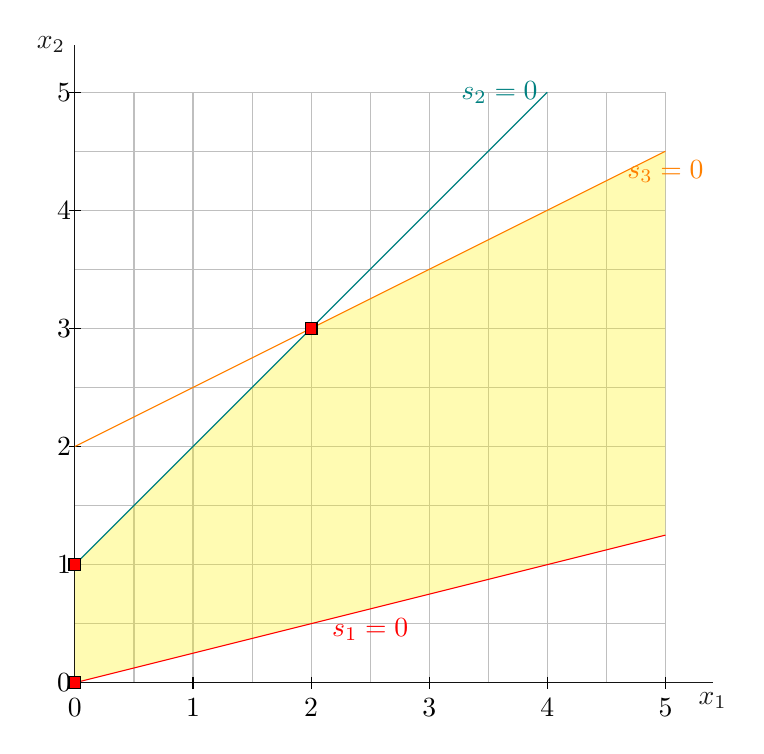
\begin{tikzpicture} [scale=1.5]
    \draw[gray!50, thin, step=.5] (0,0) grid (5,5);
    \draw[opacity=0.9] (0,0) -- (5.4,0) node[below] {$x_1$};
    \draw[opacity=0.9] (0,0) -- (0,5.4) node[left] {$x_2$}; % option \draw[very thick,->]

    \foreach \x in {0,...,5} \draw (\x,0.05) -- (\x,-0.05) node[below] {\x};
    \foreach \y in {0,...,5} \draw (-0.05,\y) -- (0.05,\y) node[left] {\y};

    \fill[yellow,opacity=0.3] (0,0) -- (0,1) -- (2,3) -- (5,4.5) --(5,1.25)-- cycle;

    \draw [red](0,0) -- node[below] {$s_1=0$} (5, 1.25);
    \draw [teal] (0,1)  --  (4,5) node[left, sloped] {$s_2=0$};
    \draw [orange](0,2) --  (5,4.5) node[below, sloped] {$s_3=0$}; %node[above right ,sloped] 
	\filldraw[fill=red] (-0.05,-0.05) rectangle (0.05,0.05);
	\filldraw[fill=red] (-0.05,.95) rectangle (0.05,1.05);
	\filldraw[fill=red] (1.95,2.95) rectangle (2.05,3.05);
\end{tikzpicture} \end{center} 
\end{minipage}

\begin{center}  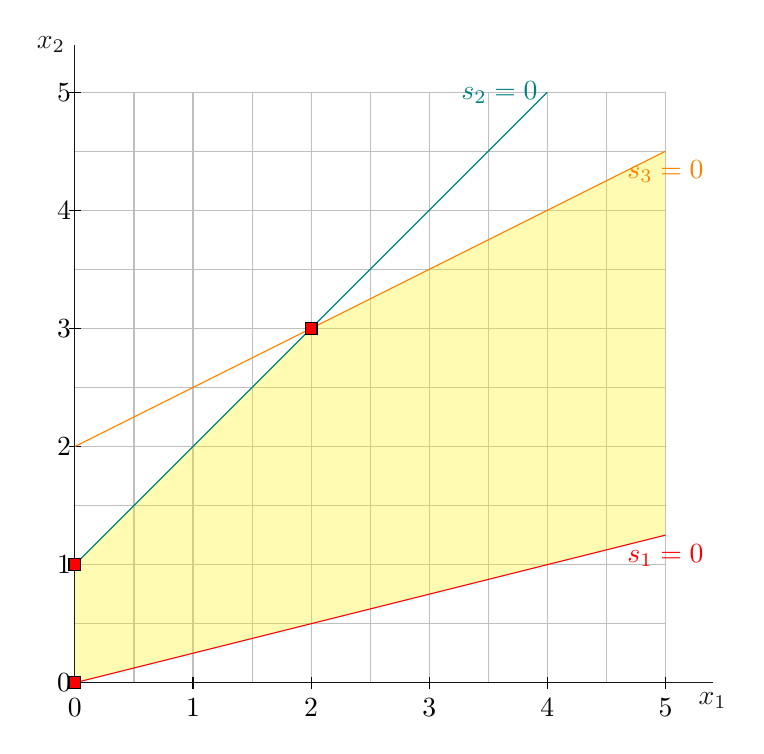
\begin{tikzpicture} [scale=1.5]
    \draw[gray!50, thin, step=.5] (0,0) grid (5,5);
    \draw[opacity=0.9] (0,0) -- (5.4,0) node[below] {$x_1$};
    \draw[opacity=0.9] (0,0) -- (0,5.4) node[left] {$x_2$}; % option \draw[very thick,->]

    \foreach \x in {0,...,5} \draw (\x,0.05) -- (\x,-0.05) node[below] {\x};
    \foreach \y in {0,...,5} \draw (-0.05,\y) -- (0.05,\y) node[left] {\y};

    \fill[yellow,opacity=0.3] (0,0) -- (0,1) -- (2,3) -- (5,4.5) --(5,1.25)-- cycle;

\draw[domain=0:4,smooth,variable=\x, teal] plot ({\x},{\x+1}) node[left] {$s_2=0$};
\draw[domain=0:5,smooth,variable=\x, red] plot ({\x},{\x*1/4}) node[below] {$s_1=0$};
%    \draw [red](0,0) -- node[below] {$s_1=0$} (5, 1.25);
    %\draw [teal] (0,1)  --  (4,5) node[left, sloped] {$s_2=0$};
    \draw [orange](0,2) --  (5,4.5) node[below, sloped] {$s_3=0$}; %node[above right ,sloped] 
	\filldraw[fill=red] (-0.05,-0.05) rectangle (0.05,0.05);
	\filldraw[fill=red] (-0.05,.95) rectangle (0.05,1.05);
	\filldraw[fill=red] (1.95,2.95) rectangle (2.05,3.05);
\end{tikzpicture} \end{center} 

% \draw[scale=0.5,domain=-3:3,smooth,variable=\x,blue] plot ({\x},{\x*\x});


\medskip E.g., consider the $s_3=0$ (orange) line, to find the extreme direction start at extreme point (2,3) and find another feasible point on the orange line, say (4,4) and subtract (2,3) from (4,4), which yields (2,1). 

\medskip This is related to the slope in two-dimensions, as discussed in class, the rise is 1 and the run is 2. So this direction has a slope of 1/2, but this does not carry over easily to higher dimensions where directions cannot be defined by a single number. 

\medskip To find the extreme directions we can change the right-hand-side to $\mathbf{b} = \mathbf{0}$, which forms a polyhedral cone (in yellow), and then add the constraint $x_1 + x_2 = 1$. The intersection of the cone and  $x_1 + x_2 = 1$ form a line segment.

\begin{minipage}[t][][b]{.4\linewidth} \vspace{0mm}
\begin{align*}
\mbox{max~~} & z = -5x_1 - x_2  \\
\mbox{s.t.~~} & x_1 - 4x_2 +s_1 = 0  \\
& -x_1 + x_2 + s_2 = 0 \\
& -x_1 + 2x_2 +s_3 = 0 \\
& x_1 + x_2 = 1 \\
& x_1, x_2, s_1, s_2, s_3 \ge 0.
\end{align*}
\end{minipage}%
\begin{minipage}[t][][b]{.6\linewidth}
\begin{center} 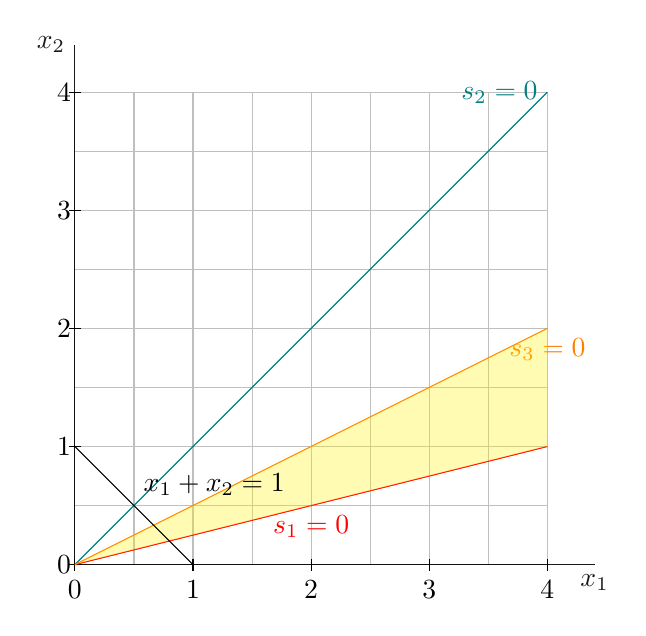
\begin{tikzpicture} [scale=1.5]
\draw[gray!50, thin, step=.5] (0,0) grid (4,4);
\draw[opacity=0.9] (0,0) -- (4.4,0) node[below] {$x_1$};
\draw[opacity=0.9] (0,0) -- (0,4.4) node[left] {$x_2$}; % option \draw[very thick,->]

\foreach \x in {0,...,4} \draw (\x,0.05) -- (\x,-0.05) node[below] {\x};
\foreach \y in {0,...,4} \draw (-0.05,\y) -- (0.05,\y) node[left] {\y};
        
\draw [red](0, 0) -- node[below] {$s_1=0$} (4, 1);
\draw [teal] (0,0)  -- (4,4) node[left, sloped] {$s_2=0$};
\draw [orange](0,0) -- (4,2) node[below, sloped] {$s_3=0$}; 
\fill[yellow,opacity=0.3] (0,0) -- (4,2) -- (4,1) --  cycle; % \draw [orange!50!blue] 

\draw [black] (0,1)  -- node[above right] {$x_1+x_2 = 1$} (1,0); 
\end{tikzpicture} \end{center} 
\end{minipage}



\begin{center} 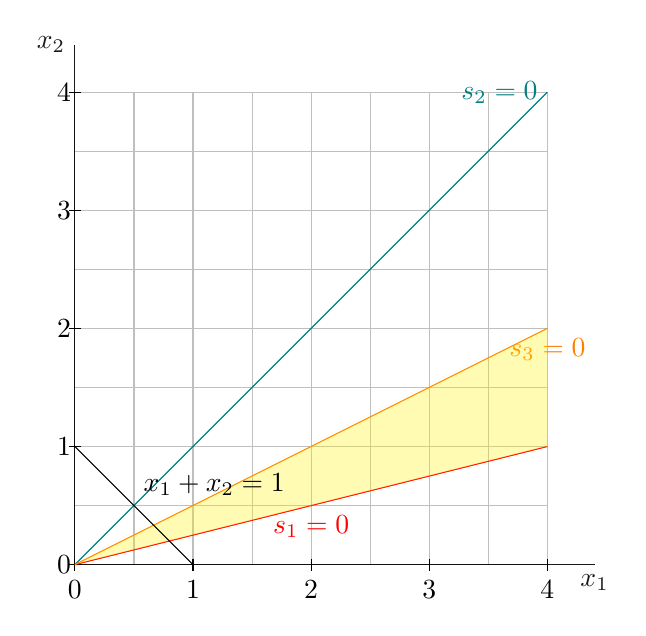
\begin{tikzpicture} [scale=1.5]
\draw[gray!50, thin, step=.5] (0,0) grid (4,4);
\draw[opacity=0.9] (0,0) -- (4.4,0) node[below] {$x_1$};
\draw[opacity=0.9] (0,0) -- (0,4.4) node[left] {$x_2$}; % option \draw[very thick,->]

\foreach \x in {0,...,4} \draw (\x,0.05) -- (\x,-0.05) node[below] {\x};
\foreach \y in {0,...,4} \draw (-0.05,\y) -- (0.05,\y) node[left] {\y};
        
\draw [red](0, 0) -- node[below] {$s_1=0$} (4, 1);
\draw [teal] (0,0)  -- (4,4) node[left, sloped] {$s_2=0$};
\draw [orange](0,0) -- (4,2) node[below, sloped] {$s_3=0$}; 
\fill[yellow,opacity=0.3] (0,0) -- (4,2) -- (4,1) --  cycle; % \draw [orange!50!blue] 

\draw [black] (0,1)  -- node[above right] {$x_1+x_2 = 1$} (1,0); 
\end{tikzpicture} \end{center} 


\medskip Magnifying for clarity, and removing the $s_2=0$ (teal) line, as it is redundant, and marking the extreme points of the new feasible region, (4/5, 1/5) and (2/3, 1/3), with red boxes, we have:

\begin{center}  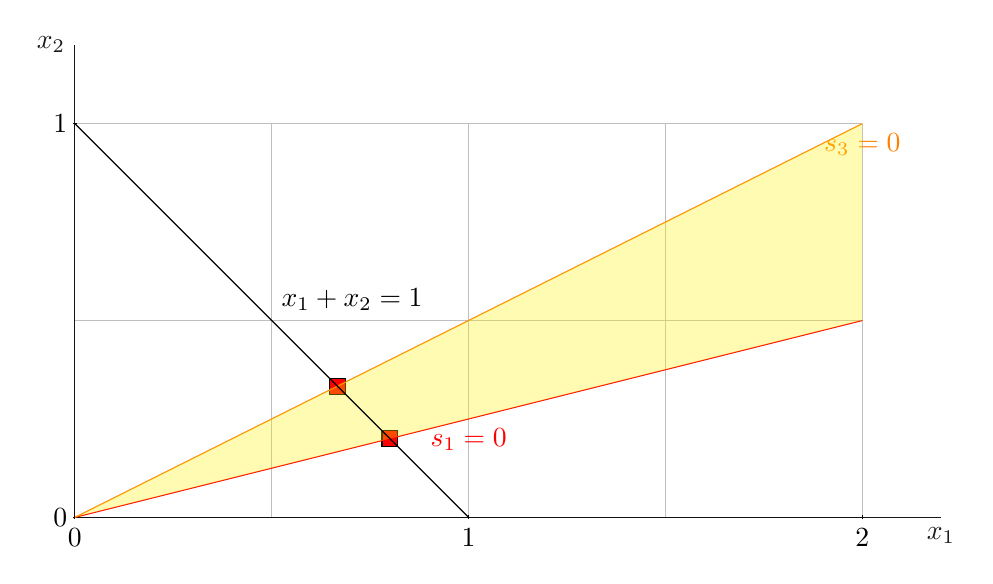
\begin{tikzpicture} [x=50mm, y=50mm] [scale=1.5]
\draw[gray!50, thin, step=.5] (0,0) grid (2,1);
\draw[opacity=0.9] (0,0) -- (2.2,0) node[below] {$x_1$};
\draw[opacity=0.9] (0,0) -- (0,1.2) node[left] {$x_2$}; % option \draw[very thick,->]

\foreach \x in {0,...,2} \draw (\x,0.005) -- (\x,-0.005) node[below] {\x};
\foreach \y in {0,...,1} \draw (-0.005,\y) -- (0.005,\y) node[left] {\y};

\filldraw[fill=red] (0.8-0.02,0.2-0.02) rectangle (0.8+0.02,0.2+0.02);
\filldraw[fill=red] (0.667-0.02,0.333-0.02) rectangle (0.667+0.02,0.333+0.02);

\draw [red](0, 0) -- node[below] {$s_1=0$} (2, .5);
\draw [orange](0,0) -- (2,1) node[below, sloped] {$s_3=0$}; 
\fill[yellow,opacity=0.3] (0,0) -- (2,.5) -- (2,1) --  cycle; % \draw [orange!50!blue] 
\draw [black] (0,1)  -- node[above right] {$x_1+x_2 = 1$} (1,0); 
\end{tikzpicture} \end{center} 

The extreme directions are thus (4/5, 1/5) and (2/3, 1/3). \\

{\bf Representation Theorem:} Let  $\mathbf{x_1}, \mathbf{x_2},\cdots \mathbf{x_k}$ be the set of extreme points of $\mathcal{S}$, and if $\mathcal{S}$ is unbounded, $\mathbf{d_1}, \mathbf{d_2},\cdots \mathbf{d_l}$ be the set of extreme directions. Then any $\mathbf{x} \in \mathcal{S}$ is equal to a convex combination of the extreme points and a non-negative linear combination of the extreme directions: $\mathbf{x} = \sum_{j=1}^k \lambda_j \mathbf{x_j} + \sum_{j=1}^l \mu_j \mathbf{d_j}$, where $\sum_{j=1}^k \lambda_j = 1$, $\lambda_j \ge 0,~\forall  j=1,2,\cdots,k$, and $\mu_j \ge 0,~\forall j=1,2,\cdots,l$.

 \begin{minipage}[t][][b]{.4\linewidth}
\begin{align*}
\mbox{max~~} & z = -5x_1 - x_2  \\\
\mbox{s.t.~~} & x_1 - 4x_2 +s_1 = 0  \\
& -x_1 + x_2 + s_2 = 1 \\
& -x_1 + 2x_2 +s_3 = 4 \\
& x_1, x_2, s_1, s_2, s_3 \ge 0.
\end{align*}
\end{minipage}%
\begin{minipage}[t][][b]{.6\linewidth}
\begin{center}  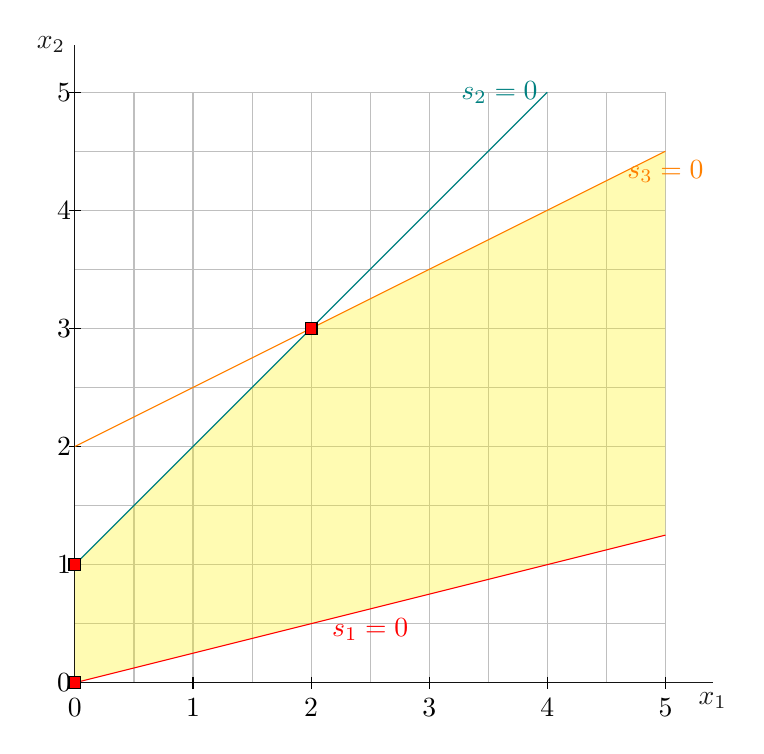
\begin{tikzpicture} [scale=1.5]
    \draw[gray!50, thin, step=.5] (0,0) grid (5,5);
    \draw[opacity=0.9] (0,0) -- (5.4,0) node[below] {$x_1$};
    \draw[opacity=0.9] (0,0) -- (0,5.4) node[left] {$x_2$}; % option \draw[very thick,->]

    \foreach \x in {0,...,5} \draw (\x,0.05) -- (\x,-0.05) node[below] {\x};
    \foreach \y in {0,...,5} \draw (-0.05,\y) -- (0.05,\y) node[left] {\y};

    \fill[yellow,opacity=0.3] (0,0) -- (0,1) -- (2,3) -- (5,4.5) --(5,1.25)-- cycle;

    \draw [red](0,0) -- node[below] {$s_1=0$} (5, 1.25);
    \draw [teal] (0,1)  --  (4,5) node[left, sloped] {$s_2=0$};
    \draw [orange](0,2) --  (5,4.5) node[below, sloped] {$s_3=0$}; %node[above right ,sloped] 
	\filldraw[fill=red] (-0.05,-0.05) rectangle (0.05,0.05);
	\filldraw[fill=red] (-0.05,.95) rectangle (0.05,1.05);
	\filldraw[fill=red] (1.95,2.95) rectangle (2.05,3.05);
\end{tikzpicture} \end{center} 
\end{minipage}

Represent point (1/2, 1) as a convex combination of the extreme points of the above LP.  Find $\lambda$s to solve the following system of equations:

$$\lambda_1 \left[
  \begin{array}{c}
  0 \\
  0 \\
  \end{array} \right]+
 \lambda_2 \left[
  \begin{array}{c}
  0 \\
  1 \\
  \end{array} \right] +
 \lambda_3 \left[
  \begin{array}{c}
  2 \\
  3 \\
  \end{array} \right]  =
 \left[
  \begin{array}{c}
  1/2 \\
  1 \\
  \end{array} \right] 
$$





\newpage 

\chapter{Software - Excel}
\todoChapter{ 10\% complete. Goal 80\% completion date: July 20\\
Notes: }
\begin{resource}
\begin{itemize}
\item \href{https://www.youtube.com/watch?v=dRm5MEoA3OI&ab_channel=LeilaGharani}{Excel Solver - Introduction on Youtube}

\item \href{https://ocw.mit.edu/courses/sloan-school-of-management/15-053-optimization-methods-in-management-science-spring-2013/tutorials/MIT15_053S13_tut03.pdf}{Some notes from MIT}
\end{itemize}
\end{resource}

\subsection{Excel Solver}
\subsection{Videos}
\href{https://www.youtube.com/watch?v=V5DmekIFenA}{Solving a linear program}
\href{https://www.youtube.com/watch?v=6xa1x_Iqjzg}{Optimal product mix}
\href{https://www.youtube.com/watch?v=vpodCzRtUMU}{Set Cover}

\href{https://www.youtube.com/watch?v=tKV24jzZ10s}{Introduction to Designing Optimization Models Using Excel Solver}

\href{https://www.youtube.com/watch?v=-E3rSoClgMI}{Traveling Salesman Problem}

\href{https://www.youtube.com/watch?v=UQYJvSjXE6I}{Also Travelin Salesman Problem}

\href{https://www.youtube.com/watch?v=owHq3Mbniqo}{Multiple Traveling Salesman Problem}

\href{https://www.youtube.com/watch?v=JkZkGxVZ8ao}{Shortest Path}

\subsection{Links}
\href{https://github.com/lobodemonte/excel-solver-loan-example}{Loan Example}

\href{https://github.com/Bhargavanarasimhan/Excel-Solver-Files}{Several Examples including TSP}


\chapter{Software - Python}
\todoChapter{ 10\% complete. Goal 80\% completion date: July 20\\
Notes: }
\begin{outcome}
\begin{itemize}
\item Install and get python up and running in some form
\item Introduce basic python skills that will be helpful
\end{itemize}
\end{outcome}

\begin{resource}
\begin{itemize}
\item\href{https://open.umn.edu/opentextbooks/textbooks/a-byte-of-python}{A Byte of Python}
\item\href{https://github.com/swaroopch/byte-of-python}{Github - Byte of Python} (CC-BY-SA)
\end{itemize}
\end{resource}

\subimport{./foundationsAppliedMathematicsLabs/Appendices/Installation/}{Installation} %Chapter
\subimport{./foundationsAppliedMathematicsLabs/Appendices/NumpyVisualGuide/}{NumpyVisualGuide} %Chapter
\subimport{./foundationsAppliedMathematicsLabs/Appendices/MatplotlibCustomization/}{MatplotlibCustomization} %Chapter

\section{Networkx - A Python Graph Algorithms Package}


\section{PuLP - An Optimization Modeling Tool for Python}
\begin{outcome}
\begin{itemize}
\item Install and import PuLP
\item Run basic first PuLP model
\item Run "advanced" PuLP model using the algebraic modeling approach and importing data.
\item Explore PuLP objects and possibilities
\item Solve a Multi-Objective problem
\end{itemize}
\end{outcome}


\begin{resource}
\begin{itemize}
\item \href{https://coin-or.github.io/pulp/}{Documentation}
\item \href{https://pypi.org/project/PuLP/}{PyPi installation}
\item \href{https://github.com/coin-or/pulp/tree/master/examples}{Examples}
\item \href{https://benalexkeen.com/linear-programming-with-python-and-pulp-part-1/}{Blog with tutorial}
\end{itemize}
\end{resource}

PuLP is an optimizaiton modeling language that is written for Python.  It is free and open source.  Yay!   See Section ?? for a discussion of other options for implementing your optimization problem.
PuLP is convenient for it's simple syntax and easy installation.   
 
Key benefits of using an algebraic modeling language like PuLP over Excel
\begin{itemize}
\item Easily readable models
\item Precompute parameters within Python
\item Reuse of common optimization models without recreating the equations
\end{itemize}

We will follow the introduction to pulp Jupyter Notebook Tutorial and the following application with a cleaner implementation.



%    \hypertarget{pulp-tutorial}{%
%\subsection{Pulp Tutorial}\label{pulp-tutorial}}

    \hypertarget{installation}{%
\subsection{Installation}\label{installation}}

Open a Jupyter notebook. In one of the cells, run the following command,
based on which system you are running. It will take a minute to load and
download the package.

    \begin{tcolorbox}[breakable, size=fbox, boxrule=1pt, pad at break*=1mm,colback=cellbackground, colframe=cellborder]
\prompt{In}{incolor}{ }{\boxspacing}
\begin{Verbatim}[commandchars=\\\{\}]
\PY{c+c1}{\PYZsh{}\PYZsh{} Install pulp (on windows)}
\PY{o}{!}pip install pulp
\end{Verbatim}
\end{tcolorbox}

    \begin{tcolorbox}[breakable, size=fbox, boxrule=1pt, pad at break*=1mm,colback=cellbackground, colframe=cellborder]
\prompt{In}{incolor}{ }{\boxspacing}
\begin{Verbatim}[commandchars=\\\{\}]
\PY{c+c1}{\PYZsh{} on a mac}
\PY{n}{pip} \PY{n}{install} \PY{n}{pulp}
\end{Verbatim}
\end{tcolorbox}

    \begin{tcolorbox}[breakable, size=fbox, boxrule=1pt, pad at break*=1mm,colback=cellbackground, colframe=cellborder]
\prompt{In}{incolor}{ }{\boxspacing}
\begin{Verbatim}[commandchars=\\\{\}]
\PY{c+c1}{\PYZsh{} on the VT ARC servers}
\PY{k+kn}{import} \PY{n+nn}{sys}
\PY{o}{!}\PY{o}{\PYZob{}}sys.executable\PY{o}{\PYZcb{}} \PYZhy{}m pip install pulp
\end{Verbatim}
\end{tcolorbox}

    \#\#\# Installation (Continued) Now restart the kernel of your notebook
(find the tab labeled Kernel in your Jupyter notebook, and in the drop
down, select restart).

    \hypertarget{example-problem}{%
\subsection{Example Problem}\label{example-problem}}

\hypertarget{product-mix-problem}{%
\subsubsection{Product Mix Problem}\label{product-mix-problem}}

\begin{align*}
  & \text{maximize }   &   Z=3&X_{1}+2X_{2}         & \text{(Objective function)} &\quad(1.1)\\[1ex]
  & \text{subject to } & \, 10&X_{1}+5X_{2} \le 300 & \text{(Constraint 1)}       &\quad(1.2)\\[1ex]
  &                    & \,  4&X_{1}+4X_{2} \le 160 & \text{(Constraint 2)}       &\quad(1.3)\\[1ex]  
  &                    & \,  2&X_{1}+6X_{2} \le 180 & \text{(Constraint 3)}       &\quad(1.4)\\[1ex] 
  & \text{and}         & \,   &X_{1},X_{2} \ge 0    & \text{(Non-negative)}       &\quad(1.5)\\[1ex] 
\end{align*}

    \hypertarget{optimization-with-pulp}{%
\paragraph{Optimization with PuLP}\label{optimization-with-pulp}}

    \begin{tcolorbox}[breakable, size=fbox, boxrule=1pt, pad at break*=1mm,colback=cellbackground, colframe=cellborder]
\prompt{In}{incolor}{1}{\boxspacing}
\begin{Verbatim}[commandchars=\\\{\}]
\PY{k+kn}{from} \PY{n+nn}{pulp} \PY{k+kn}{import} \PY{o}{*}

\PY{c+c1}{\PYZsh{} Define problem}
\PY{n}{prob} \PY{o}{=} \PY{n}{LpProblem}\PY{p}{(}\PY{n}{name}\PY{o}{=}\PY{l+s+s1}{\PYZsq{}}\PY{l+s+s1}{Product\PYZus{}Mix\PYZus{}Problem}\PY{l+s+s1}{\PYZsq{}}\PY{p}{,} \PY{n}{sense}\PY{o}{=}\PY{n}{LpMaximize}\PY{p}{)}

\PY{c+c1}{\PYZsh{} Create decision variables and non\PYZhy{}negative constraint}
\PY{n}{x1} \PY{o}{=} \PY{n}{LpVariable}\PY{p}{(}\PY{n}{name}\PY{o}{=}\PY{l+s+s1}{\PYZsq{}}\PY{l+s+s1}{X1}\PY{l+s+s1}{\PYZsq{}}\PY{p}{,} \PY{n}{lowBound}\PY{o}{=}\PY{l+m+mi}{0}\PY{p}{,} \PY{n}{upBound}\PY{o}{=}\PY{k+kc}{None}\PY{p}{,} \PY{n}{cat}\PY{o}{=}\PY{l+s+s1}{\PYZsq{}}\PY{l+s+s1}{Continuous}\PY{l+s+s1}{\PYZsq{}}\PY{p}{)}
\PY{n}{x2} \PY{o}{=} \PY{n}{LpVariable}\PY{p}{(}\PY{n}{name}\PY{o}{=}\PY{l+s+s1}{\PYZsq{}}\PY{l+s+s1}{X2}\PY{l+s+s1}{\PYZsq{}}\PY{p}{,} \PY{n}{lowBound}\PY{o}{=}\PY{l+m+mi}{0}\PY{p}{,} \PY{n}{upBound}\PY{o}{=}\PY{k+kc}{None}\PY{p}{,} \PY{n}{cat}\PY{o}{=}\PY{l+s+s1}{\PYZsq{}}\PY{l+s+s1}{Continuous}\PY{l+s+s1}{\PYZsq{}}\PY{p}{)}

\PY{c+c1}{\PYZsh{} Set objective function}
\PY{n}{prob} \PY{o}{+}\PY{o}{=} \PY{l+m+mi}{3}\PY{o}{*}\PY{n}{x1} \PY{o}{+} \PY{l+m+mi}{2}\PY{o}{*}\PY{n}{x2}

\PY{c+c1}{\PYZsh{} Set constraints}
\PY{n}{prob} \PY{o}{+}\PY{o}{=} \PY{l+m+mi}{10}\PY{o}{*}\PY{n}{x1} \PY{o}{+} \PY{l+m+mi}{5}\PY{o}{*}\PY{n}{x2} \PY{o}{\PYZlt{}}\PY{o}{=} \PY{l+m+mi}{300}
\PY{n}{prob} \PY{o}{+}\PY{o}{=} \PY{l+m+mi}{4}\PY{o}{*}\PY{n}{x1} \PY{o}{+} \PY{l+m+mi}{4}\PY{o}{*}\PY{n}{x2} \PY{o}{\PYZlt{}}\PY{o}{=} \PY{l+m+mi}{160}
\PY{n}{prob} \PY{o}{+}\PY{o}{=} \PY{l+m+mi}{2}\PY{o}{*}\PY{n}{x1} \PY{o}{+} \PY{l+m+mi}{6}\PY{o}{*}\PY{n}{x2} \PY{o}{\PYZlt{}}\PY{o}{=} \PY{l+m+mi}{180}

\PY{c+c1}{\PYZsh{} Solving problem}
\PY{n}{prob}\PY{o}{.}\PY{n}{solve}\PY{p}{(}\PY{p}{)}
\PY{n+nb}{print}\PY{p}{(}\PY{l+s+s1}{\PYZsq{}}\PY{l+s+s1}{Status}\PY{l+s+s1}{\PYZsq{}}\PY{p}{,} \PY{n}{LpStatus}\PY{p}{[}\PY{n}{prob}\PY{o}{.}\PY{n}{status}\PY{p}{]}\PY{p}{)}
\end{Verbatim}
\end{tcolorbox}

    \begin{Verbatim}[commandchars=\\\{\}]
Status Optimal
    \end{Verbatim}

    \begin{tcolorbox}[breakable, size=fbox, boxrule=1pt, pad at break*=1mm,colback=cellbackground, colframe=cellborder]
\prompt{In}{incolor}{2}{\boxspacing}
\begin{Verbatim}[commandchars=\\\{\}]
\PY{n+nb}{print}\PY{p}{(}\PY{l+s+s2}{\PYZdq{}}\PY{l+s+s2}{Status:}\PY{l+s+s2}{\PYZdq{}}\PY{p}{,} \PY{n}{LpStatus}\PY{p}{[}\PY{n}{prob}\PY{o}{.}\PY{n}{status}\PY{p}{]}\PY{p}{)}
\PY{n+nb}{print}\PY{p}{(}\PY{l+s+s2}{\PYZdq{}}\PY{l+s+s2}{Objective value: }\PY{l+s+s2}{\PYZdq{}}\PY{p}{,} \PY{n}{prob}\PY{o}{.}\PY{n}{objective}\PY{o}{.}\PY{n}{value}\PY{p}{(}\PY{p}{)}\PY{p}{)}

\PY{k}{for} \PY{n}{v} \PY{o+ow}{in} \PY{n}{prob}\PY{o}{.}\PY{n}{variables}\PY{p}{(}\PY{p}{)}\PY{p}{:}
    \PY{n+nb}{print}\PY{p}{(}\PY{n}{v}\PY{o}{.}\PY{n}{name}\PY{p}{,}\PY{l+s+s1}{\PYZsq{}}\PY{l+s+s1}{: }\PY{l+s+s1}{\PYZsq{}}\PY{p}{,} \PY{n}{v}\PY{o}{.}\PY{n}{value}\PY{p}{(}\PY{p}{)}\PY{p}{)}
\end{Verbatim}
\end{tcolorbox}

    \begin{Verbatim}[commandchars=\\\{\}]
Status: Optimal
Objective value:  100.0
X1 :  20.0
X2 :  20.0
    \end{Verbatim}

    \hypertarget{things-we-can-do}{%
\subsection{Things we can do}\label{things-we-can-do}}

    \begin{tcolorbox}[breakable, size=fbox, boxrule=1pt, pad at break*=1mm,colback=cellbackground, colframe=cellborder]
\prompt{In}{incolor}{3}{\boxspacing}
\begin{Verbatim}[commandchars=\\\{\}]
\PY{c+c1}{\PYZsh{} print the problem}
\PY{n}{prob}
\end{Verbatim}
\end{tcolorbox}

            \begin{tcolorbox}[breakable, size=fbox, boxrule=.5pt, pad at break*=1mm, opacityfill=0]
\prompt{Out}{outcolor}{3}{\boxspacing}
\begin{Verbatim}[commandchars=\\\{\}]
Product\_Mix\_Problem:
MAXIMIZE
3*X1 + 2*X2 + 0
SUBJECT TO
\_C1: 10 X1 + 5 X2 <= 300

\_C2: 4 X1 + 4 X2 <= 160

\_C3: 2 X1 + 6 X2 <= 180

VARIABLES
X1 Continuous
X2 Continuous
\end{Verbatim}
\end{tcolorbox}
        
    \begin{tcolorbox}[breakable, size=fbox, boxrule=1pt, pad at break*=1mm,colback=cellbackground, colframe=cellborder]
\prompt{In}{incolor}{4}{\boxspacing}
\begin{Verbatim}[commandchars=\\\{\}]
\PY{c+c1}{\PYZsh{} get the objective function}
\PY{n}{prob}\PY{o}{.}\PY{n}{objective}\PY{o}{.}\PY{n}{value}\PY{p}{(}\PY{p}{)}
\end{Verbatim}
\end{tcolorbox}

            \begin{tcolorbox}[breakable, size=fbox, boxrule=.5pt, pad at break*=1mm, opacityfill=0]
\prompt{Out}{outcolor}{4}{\boxspacing}
\begin{Verbatim}[commandchars=\\\{\}]
100.0
\end{Verbatim}
\end{tcolorbox}
        
    \begin{tcolorbox}[breakable, size=fbox, boxrule=1pt, pad at break*=1mm,colback=cellbackground, colframe=cellborder]
\prompt{In}{incolor}{5}{\boxspacing}
\begin{Verbatim}[commandchars=\\\{\}]
\PY{c+c1}{\PYZsh{} get list of the variables}
\PY{n}{prob}\PY{o}{.}\PY{n}{variables}\PY{p}{(}\PY{p}{)}
\end{Verbatim}
\end{tcolorbox}

            \begin{tcolorbox}[breakable, size=fbox, boxrule=.5pt, pad at break*=1mm, opacityfill=0]
\prompt{Out}{outcolor}{5}{\boxspacing}
\begin{Verbatim}[commandchars=\\\{\}]
[X1, X2]
\end{Verbatim}
\end{tcolorbox}
        
    \begin{tcolorbox}[breakable, size=fbox, boxrule=1pt, pad at break*=1mm,colback=cellbackground, colframe=cellborder]
\prompt{In}{incolor}{6}{\boxspacing}
\begin{Verbatim}[commandchars=\\\{\}]
\PY{k}{for} \PY{n}{v} \PY{o+ow}{in} \PY{n}{prob}\PY{o}{.}\PY{n}{variables}\PY{p}{(}\PY{p}{)}\PY{p}{:}
    \PY{n+nb}{print}\PY{p}{(}\PY{l+s+sa}{f}\PY{l+s+s1}{\PYZsq{}}\PY{l+s+si}{\PYZob{}}\PY{n}{v}\PY{l+s+si}{\PYZcb{}}\PY{l+s+s1}{: }\PY{l+s+si}{\PYZob{}}\PY{n}{v}\PY{o}{.}\PY{n}{varValue}\PY{l+s+si}{\PYZcb{}}\PY{l+s+s1}{\PYZsq{}}\PY{p}{)}
\end{Verbatim}
\end{tcolorbox}

    \begin{Verbatim}[commandchars=\\\{\}]
X1: 20.0
X2: 20.0
    \end{Verbatim}

    \hypertarget{exploring-the-variables}{%
\subsubsection{Exploring the variables}\label{exploring-the-variables}}

    \begin{tcolorbox}[breakable, size=fbox, boxrule=1pt, pad at break*=1mm,colback=cellbackground, colframe=cellborder]
\prompt{In}{incolor}{7}{\boxspacing}
\begin{Verbatim}[commandchars=\\\{\}]
\PY{n}{v} \PY{o}{=} \PY{n}{prob}\PY{o}{.}\PY{n}{variables}\PY{p}{(}\PY{p}{)}\PY{p}{[}\PY{l+m+mi}{0}\PY{p}{]}
\end{Verbatim}
\end{tcolorbox}

    \begin{tcolorbox}[breakable, size=fbox, boxrule=1pt, pad at break*=1mm,colback=cellbackground, colframe=cellborder]
\prompt{In}{incolor}{9}{\boxspacing}
\begin{Verbatim}[commandchars=\\\{\}]
\PY{n}{v}\PY{o}{.}\PY{n}{name}
\end{Verbatim}
\end{tcolorbox}

            \begin{tcolorbox}[breakable, size=fbox, boxrule=.5pt, pad at break*=1mm, opacityfill=0]
\prompt{Out}{outcolor}{9}{\boxspacing}
\begin{Verbatim}[commandchars=\\\{\}]
'X1'
\end{Verbatim}
\end{tcolorbox}
        
    \begin{tcolorbox}[breakable, size=fbox, boxrule=1pt, pad at break*=1mm,colback=cellbackground, colframe=cellborder]
\prompt{In}{incolor}{10}{\boxspacing}
\begin{Verbatim}[commandchars=\\\{\}]
\PY{n}{v}\PY{o}{.}\PY{n}{value}\PY{p}{(}\PY{p}{)}
\end{Verbatim}
\end{tcolorbox}

            \begin{tcolorbox}[breakable, size=fbox, boxrule=.5pt, pad at break*=1mm, opacityfill=0]
\prompt{Out}{outcolor}{10}{\boxspacing}
\begin{Verbatim}[commandchars=\\\{\}]
20.0
\end{Verbatim}
\end{tcolorbox}
        
    \begin{tcolorbox}[breakable, size=fbox, boxrule=1pt, pad at break*=1mm,colback=cellbackground, colframe=cellborder]
\prompt{In}{incolor}{11}{\boxspacing}
\begin{Verbatim}[commandchars=\\\{\}]
\PY{n}{v}\PY{o}{.}\PY{n}{varValue}
\end{Verbatim}
\end{tcolorbox}

            \begin{tcolorbox}[breakable, size=fbox, boxrule=.5pt, pad at break*=1mm, opacityfill=0]
\prompt{Out}{outcolor}{11}{\boxspacing}
\begin{Verbatim}[commandchars=\\\{\}]
20.0
\end{Verbatim}
\end{tcolorbox}
        
    \hypertarget{other-things-you-can-do}{%
\subsubsection{Other things you can do}\label{other-things-you-can-do}}

    \begin{tcolorbox}[breakable, size=fbox, boxrule=1pt, pad at break*=1mm,colback=cellbackground, colframe=cellborder]
\prompt{In}{incolor}{12}{\boxspacing}
\begin{Verbatim}[commandchars=\\\{\}]
\PY{c+c1}{\PYZsh{} get list of the constraints}
\PY{n}{prob}\PY{o}{.}\PY{n}{constraints}
\end{Verbatim}
\end{tcolorbox}

            \begin{tcolorbox}[breakable, size=fbox, boxrule=.5pt, pad at break*=1mm, opacityfill=0]
\prompt{Out}{outcolor}{12}{\boxspacing}
\begin{Verbatim}[commandchars=\\\{\}]
OrderedDict([('\_C1', 10*X1 + 5*X2 + -300 <= 0),
             ('\_C2', 4*X1 + 4*X2 + -160 <= 0),
             ('\_C3', 2*X1 + 6*X2 + -180 <= 0)])
\end{Verbatim}
\end{tcolorbox}
        
    \begin{tcolorbox}[breakable, size=fbox, boxrule=1pt, pad at break*=1mm,colback=cellbackground, colframe=cellborder]
\prompt{In}{incolor}{13}{\boxspacing}
\begin{Verbatim}[commandchars=\\\{\}]
\PY{n}{prob}\PY{o}{.}\PY{n}{to\PYZus{}dict}\PY{p}{(}\PY{p}{)}
\end{Verbatim}
\end{tcolorbox}

            \begin{tcolorbox}[breakable, size=fbox, boxrule=.5pt, pad at break*=1mm, opacityfill=0]
\prompt{Out}{outcolor}{13}{\boxspacing}
\begin{Verbatim}[commandchars=\\\{\}]
\{'objective': \{'name': 'OBJ',
  'coefficients': [\{'name': 'X1', 'value': 3\}, \{'name': 'X2', 'value': 2\}]\},
 'constraints': [\{'sense': -1,
   'pi': 0.2,
   'constant': -300,
   'name': None,
   'coefficients': [\{'name': 'X1', 'value': 10\}, \{'name': 'X2', 'value': 5\}]\},
  \{'sense': -1,
   'pi': 0.25,
   'constant': -160,
   'name': None,
   'coefficients': [\{'name': 'X1', 'value': 4\}, \{'name': 'X2', 'value': 4\}]\},
  \{'sense': -1,
   'pi': -0.0,
   'constant': -180,
   'name': None,
   'coefficients': [\{'name': 'X1', 'value': 2\}, \{'name': 'X2', 'value': 6\}]\}],
 'variables': [\{'lowBound': 0,
   'upBound': None,
   'cat': 'Continuous',
   'varValue': 20.0,
   'dj': -0.0,
   'name': 'X1'\},
  \{'lowBound': 0,
   'upBound': None,
   'cat': 'Continuous',
   'varValue': 20.0,
   'dj': -0.0,
   'name': 'X2'\}],
 'parameters': \{'name': 'Product\_Mix\_Problem',
  'sense': -1,
  'status': 1,
  'sol\_status': 1\},
 'sos1': [],
 'sos2': []\}
\end{Verbatim}
\end{tcolorbox}
        
    \begin{tcolorbox}[breakable, size=fbox, boxrule=1pt, pad at break*=1mm,colback=cellbackground, colframe=cellborder]
\prompt{In}{incolor}{15}{\boxspacing}
\begin{Verbatim}[commandchars=\\\{\}]
\PY{c+c1}{\PYZsh{} Store problem information in a json}
\PY{n}{prob}\PY{o}{.}\PY{n}{to\PYZus{}json}\PY{p}{(}\PY{l+s+s1}{\PYZsq{}}\PY{l+s+s1}{Product\PYZus{}Mix\PYZus{}Problem.json}\PY{l+s+s1}{\PYZsq{}}\PY{p}{)}
\end{Verbatim}
\end{tcolorbox}

    \hypertarget{common-issue}{%
\subsection{Common issue}\label{common-issue}}

If you forget the \textless=, ==, or \textgreater= when writing a
constraint, you will silently overwrite the objective function instead
of adding a constraint!






\hypertarget{transportation-problem}{%
\subsubsection{Transportation Problem}\label{transportation-problem}}

Transport programming is a special form of linear programming, and in
general, the objective function is cost minimization. The formula form
and applicable variables of the Transport Planning Act are as follows.
When supply and demand match, the constraint becomes an equation, but
when supply and demand do not match, the constraint becomes an
inequality.

Sets: - J = set of demand nodes - I = set of supply nodes

Parameters: 
\begin{itemize}
\item  $D_j$: Demand at node $j$ 
\item  $S_i$: Supply from node i 
\item  $c_{ij}$:
cost per unit to send supply i to demand j
\end{itemize}

Variables: 
\begin{itemize}
\item  X\_ij: Transport volume from supply \(i\) to demand \(j\)
(units)
\end{itemize}

\begin{itemize}
\item
  Objective function: \[\min \sum_{i=1}^n\sum_{j=1}^mc_{ij}x_{ij}\]
\item
  Constraints:
  \[\sum_{i=1}^nx_{ij}=S_i\]
  \[\sum_{i=1}^mx_{ij}=D_j\]
 \[ x_{ij}\geq 0 \text{ for } i \in I, j \in J\]
\end{itemize}

    \hypertarget{optimization-with-pulp}{%
\subsubsection{Optimization with PuLP}\label{optimization-with-pulp}}

Here we do a very basic implementation of the problem

    \begin{tcolorbox}[breakable, size=fbox, boxrule=1pt, pad at break*=1mm,colback=cellbackground, colframe=cellborder]
\prompt{In}{incolor}{1}{\boxspacing}
\begin{Verbatim}[commandchars=\\\{\}]
\PY{k+kn}{from} \PY{n+nn}{pulp} \PY{k+kn}{import} \PY{o}{*}

\PY{n}{prob} \PY{o}{=} \PY{n}{LpProblem}\PY{p}{(}\PY{l+s+s1}{\PYZsq{}}\PY{l+s+s1}{Transportation\PYZus{}Problem}\PY{l+s+s1}{\PYZsq{}}\PY{p}{,} \PY{n}{LpMinimize}\PY{p}{)}

\PY{n}{x11} \PY{o}{=} \PY{n}{LpVariable}\PY{p}{(}\PY{l+s+s1}{\PYZsq{}}\PY{l+s+s1}{X11}\PY{l+s+s1}{\PYZsq{}}\PY{p}{,} \PY{n}{lowBound}\PY{o}{=}\PY{l+m+mi}{0}\PY{p}{)}
\PY{n}{x12} \PY{o}{=} \PY{n}{LpVariable}\PY{p}{(}\PY{l+s+s1}{\PYZsq{}}\PY{l+s+s1}{X12}\PY{l+s+s1}{\PYZsq{}}\PY{p}{,} \PY{n}{lowBound}\PY{o}{=}\PY{l+m+mi}{0}\PY{p}{)}
\PY{n}{x13} \PY{o}{=} \PY{n}{LpVariable}\PY{p}{(}\PY{l+s+s1}{\PYZsq{}}\PY{l+s+s1}{X13}\PY{l+s+s1}{\PYZsq{}}\PY{p}{,} \PY{n}{lowBound}\PY{o}{=}\PY{l+m+mi}{0}\PY{p}{)}
\PY{n}{x14} \PY{o}{=} \PY{n}{LpVariable}\PY{p}{(}\PY{l+s+s1}{\PYZsq{}}\PY{l+s+s1}{X14}\PY{l+s+s1}{\PYZsq{}}\PY{p}{,} \PY{n}{lowBound}\PY{o}{=}\PY{l+m+mi}{0}\PY{p}{)}
\PY{n}{x21} \PY{o}{=} \PY{n}{LpVariable}\PY{p}{(}\PY{l+s+s1}{\PYZsq{}}\PY{l+s+s1}{X21}\PY{l+s+s1}{\PYZsq{}}\PY{p}{,} \PY{n}{lowBound}\PY{o}{=}\PY{l+m+mi}{0}\PY{p}{)}
\PY{n}{x22} \PY{o}{=} \PY{n}{LpVariable}\PY{p}{(}\PY{l+s+s1}{\PYZsq{}}\PY{l+s+s1}{X22}\PY{l+s+s1}{\PYZsq{}}\PY{p}{,} \PY{n}{lowBound}\PY{o}{=}\PY{l+m+mi}{0}\PY{p}{)}
\PY{n}{x23} \PY{o}{=} \PY{n}{LpVariable}\PY{p}{(}\PY{l+s+s1}{\PYZsq{}}\PY{l+s+s1}{X23}\PY{l+s+s1}{\PYZsq{}}\PY{p}{,} \PY{n}{lowBound}\PY{o}{=}\PY{l+m+mi}{0}\PY{p}{)}
\PY{n}{x24} \PY{o}{=} \PY{n}{LpVariable}\PY{p}{(}\PY{l+s+s1}{\PYZsq{}}\PY{l+s+s1}{X24}\PY{l+s+s1}{\PYZsq{}}\PY{p}{,} \PY{n}{lowBound}\PY{o}{=}\PY{l+m+mi}{0}\PY{p}{)}
\PY{n}{x31} \PY{o}{=} \PY{n}{LpVariable}\PY{p}{(}\PY{l+s+s1}{\PYZsq{}}\PY{l+s+s1}{X31}\PY{l+s+s1}{\PYZsq{}}\PY{p}{,} \PY{n}{lowBound}\PY{o}{=}\PY{l+m+mi}{0}\PY{p}{)}
\PY{n}{x32} \PY{o}{=} \PY{n}{LpVariable}\PY{p}{(}\PY{l+s+s1}{\PYZsq{}}\PY{l+s+s1}{X32}\PY{l+s+s1}{\PYZsq{}}\PY{p}{,} \PY{n}{lowBound}\PY{o}{=}\PY{l+m+mi}{0}\PY{p}{)}
\PY{n}{x33} \PY{o}{=} \PY{n}{LpVariable}\PY{p}{(}\PY{l+s+s1}{\PYZsq{}}\PY{l+s+s1}{X33}\PY{l+s+s1}{\PYZsq{}}\PY{p}{,} \PY{n}{lowBound}\PY{o}{=}\PY{l+m+mi}{0}\PY{p}{)}
\PY{n}{x34} \PY{o}{=} \PY{n}{LpVariable}\PY{p}{(}\PY{l+s+s1}{\PYZsq{}}\PY{l+s+s1}{X34}\PY{l+s+s1}{\PYZsq{}}\PY{p}{,} \PY{n}{lowBound}\PY{o}{=}\PY{l+m+mi}{0}\PY{p}{)}

\PY{n}{prob} \PY{o}{+}\PY{o}{=} \PY{l+m+mi}{4}\PY{o}{*}\PY{n}{x11} \PY{o}{+} \PY{l+m+mi}{5}\PY{o}{*}\PY{n}{x12} \PY{o}{+} \PY{l+m+mi}{6}\PY{o}{*}\PY{n}{x13} \PY{o}{+} \PY{l+m+mi}{8}\PY{o}{*}\PY{n}{x14} \PY{o}{+} \PY{l+m+mi}{4}\PY{o}{*}\PY{n}{x21} \PY{o}{+} \PY{l+m+mi}{7}\PY{o}{*}\PY{n}{x22} \PY{o}{+} \PY{l+m+mi}{9}\PY{o}{*}\PY{n}{x23} \PY{o}{+} \PY{l+m+mi}{2}\PY{o}{*}\PY{n}{x24} \PY{o}{+} \PY{l+m+mi}{5}\PY{o}{*}\PY{n}{x31} \PY{o}{+} \PY{l+m+mi}{8}\PY{o}{*}\PY{n}{x32} \PY{o}{+} \PY{l+m+mi}{7}\PY{o}{*}\PY{n}{x33} \PY{o}{+} \PY{l+m+mi}{6}\PY{o}{*}\PY{n}{x34}

\PY{n}{prob} \PY{o}{+}\PY{o}{=} \PY{n}{x11} \PY{o}{+} \PY{n}{x12} \PY{o}{+} \PY{n}{x13} \PY{o}{+} \PY{n}{x14} \PY{o}{==} \PY{l+m+mi}{120}
\PY{n}{prob} \PY{o}{+}\PY{o}{=} \PY{n}{x21} \PY{o}{+} \PY{n}{x22} \PY{o}{+} \PY{n}{x23} \PY{o}{+} \PY{n}{x24} \PY{o}{==} \PY{l+m+mi}{150}
\PY{n}{prob} \PY{o}{+}\PY{o}{=} \PY{n}{x31} \PY{o}{+} \PY{n}{x32} \PY{o}{+} \PY{n}{x33} \PY{o}{+} \PY{n}{x34} \PY{o}{==} \PY{l+m+mi}{200}

\PY{n}{prob} \PY{o}{+}\PY{o}{=} \PY{n}{x11} \PY{o}{+} \PY{n}{x21} \PY{o}{+} \PY{n}{x31} \PY{o}{==} \PY{l+m+mi}{100}
\PY{n}{prob} \PY{o}{+}\PY{o}{=} \PY{n}{x12} \PY{o}{+} \PY{n}{x22} \PY{o}{+} \PY{n}{x32} \PY{o}{==} \PY{l+m+mi}{60}
\PY{n}{prob} \PY{o}{+}\PY{o}{=} \PY{n}{x13} \PY{o}{+} \PY{n}{x23} \PY{o}{+} \PY{n}{x33} \PY{o}{==} \PY{l+m+mi}{130}
\PY{n}{prob} \PY{o}{+}\PY{o}{=} \PY{n}{x14} \PY{o}{+} \PY{n}{x24} \PY{o}{+} \PY{n}{x34} \PY{o}{==} \PY{l+m+mi}{180}

\PY{c+c1}{\PYZsh{} Solving problem}
\PY{n}{prob}\PY{o}{.}\PY{n}{solve}\PY{p}{(}\PY{p}{)}\PY{p}{;}
\end{Verbatim}
\end{tcolorbox}

    \begin{tcolorbox}[breakable, size=fbox, boxrule=1pt, pad at break*=1mm,colback=cellbackground, colframe=cellborder]
\prompt{In}{incolor}{2}{\boxspacing}
\begin{Verbatim}[commandchars=\\\{\}]
\PY{n+nb}{print}\PY{p}{(}\PY{l+s+s2}{\PYZdq{}}\PY{l+s+s2}{Status:}\PY{l+s+s2}{\PYZdq{}}\PY{p}{,} \PY{n}{LpStatus}\PY{p}{[}\PY{n}{prob}\PY{o}{.}\PY{n}{status}\PY{p}{]}\PY{p}{)}
\PY{n+nb}{print}\PY{p}{(}\PY{l+s+s2}{\PYZdq{}}\PY{l+s+s2}{Objective value: }\PY{l+s+s2}{\PYZdq{}}\PY{p}{,} \PY{n}{prob}\PY{o}{.}\PY{n}{objective}\PY{o}{.}\PY{n}{value}\PY{p}{(}\PY{p}{)}\PY{p}{)}

\PY{k}{for} \PY{n}{v} \PY{o+ow}{in} \PY{n}{prob}\PY{o}{.}\PY{n}{variables}\PY{p}{(}\PY{p}{)}\PY{p}{:}
    \PY{n+nb}{print}\PY{p}{(}\PY{n}{v}\PY{o}{.}\PY{n}{name}\PY{p}{,}\PY{l+s+s1}{\PYZsq{}}\PY{l+s+s1}{: }\PY{l+s+s1}{\PYZsq{}}\PY{p}{,} \PY{n}{v}\PY{o}{.}\PY{n}{value}\PY{p}{(}\PY{p}{)}\PY{p}{)}
\end{Verbatim}
\end{tcolorbox}

    \begin{Verbatim}[commandchars=\\\{\}]
Status: Optimal
Objective value:  2130.0
X11 :  60.0
X12 :  60.0
X13 :  0.0
X14 :  0.0
X21 :  0.0
X22 :  0.0
X23 :  0.0
X24 :  150.0
X31 :  40.0
X32 :  0.0
X33 :  130.0
X34 :  30.0
    \end{Verbatim}

    \hypertarget{optimization-with-pulp-round-2}{%
\subsubsection{Optimization with PuLP: Round
2!}\label{optimization-with-pulp-round-2}}

We now use set notation for this implementation

    \begin{tcolorbox}[breakable, size=fbox, boxrule=1pt, pad at break*=1mm,colback=cellbackground, colframe=cellborder]
\prompt{In}{incolor}{3}{\boxspacing}
\begin{Verbatim}[commandchars=\\\{\}]
\PY{k+kn}{from} \PY{n+nn}{pulp} \PY{k+kn}{import} \PY{o}{*}

\PY{n}{prob} \PY{o}{=} \PY{n}{LpProblem}\PY{p}{(}\PY{l+s+s1}{\PYZsq{}}\PY{l+s+s1}{Transportation\PYZus{}Problem}\PY{l+s+s1}{\PYZsq{}}\PY{p}{,} \PY{n}{LpMinimize}\PY{p}{)}


\PY{c+c1}{\PYZsh{} Sets}
\PY{n}{n\PYZus{}suppliers} \PY{o}{=} \PY{l+m+mi}{3}
\PY{n}{n\PYZus{}buyers} \PY{o}{=} \PY{l+m+mi}{4}

\PY{n}{I} \PY{o}{=} \PY{n+nb}{range}\PY{p}{(}\PY{n}{n\PYZus{}suppliers}\PY{p}{)}
\PY{n}{J} \PY{o}{=} \PY{n+nb}{range}\PY{p}{(}\PY{n}{n\PYZus{}buyers}\PY{p}{)}

\PY{n}{routes} \PY{o}{=} \PY{p}{[}\PY{p}{(}\PY{n}{i}\PY{p}{,} \PY{n}{j}\PY{p}{)} \PY{k}{for} \PY{n}{i} \PY{o+ow}{in} \PY{n}{I} \PY{k}{for} \PY{n}{j} \PY{o+ow}{in} \PY{n}{J}\PY{p}{]}


\PY{c+c1}{\PYZsh{} Parameters}
\PY{n}{costs} \PY{o}{=} \PY{p}{[}
    \PY{p}{[}\PY{l+m+mi}{4}\PY{p}{,} \PY{l+m+mi}{5}\PY{p}{,} \PY{l+m+mi}{6}\PY{p}{,} \PY{l+m+mi}{8}\PY{p}{]}\PY{p}{,}
    \PY{p}{[}\PY{l+m+mi}{4}\PY{p}{,} \PY{l+m+mi}{7}\PY{p}{,} \PY{l+m+mi}{9}\PY{p}{,} \PY{l+m+mi}{2}\PY{p}{]}\PY{p}{,} 
    \PY{p}{[}\PY{l+m+mi}{5}\PY{p}{,} \PY{l+m+mi}{8}\PY{p}{,} \PY{l+m+mi}{7}\PY{p}{,} \PY{l+m+mi}{6}\PY{p}{]}
\PY{p}{]}

\PY{n}{supply} \PY{o}{=} \PY{p}{[}\PY{l+m+mi}{120}\PY{p}{,} \PY{l+m+mi}{150}\PY{p}{,} \PY{l+m+mi}{200}\PY{p}{]}
\PY{n}{demand} \PY{o}{=} \PY{p}{[}\PY{l+m+mi}{100}\PY{p}{,} \PY{l+m+mi}{60}\PY{p}{,} \PY{l+m+mi}{130}\PY{p}{,} \PY{l+m+mi}{180}\PY{p}{]}



\PY{c+c1}{\PYZsh{} Variables}
\PY{n}{x} \PY{o}{=} \PY{n}{LpVariable}\PY{o}{.}\PY{n}{dicts}\PY{p}{(}\PY{l+s+s1}{\PYZsq{}}\PY{l+s+s1}{X}\PY{l+s+s1}{\PYZsq{}}\PY{p}{,} \PY{n}{routes}\PY{p}{,} \PY{n}{lowBound}\PY{o}{=}\PY{l+m+mi}{0}\PY{p}{)}

\PY{c+c1}{\PYZsh{} Objective}
\PY{n}{prob} \PY{o}{+}\PY{o}{=} \PY{n}{lpSum}\PY{p}{(}\PY{p}{[}\PY{n}{x}\PY{p}{[}\PY{n}{i}\PY{p}{,} \PY{n}{j}\PY{p}{]} \PY{o}{*} \PY{n}{costs}\PY{p}{[}\PY{n}{i}\PY{p}{]}\PY{p}{[}\PY{n}{j}\PY{p}{]} \PY{k}{for} \PY{n}{i} \PY{o+ow}{in} \PY{n}{I} \PY{k}{for} \PY{n}{j} \PY{o+ow}{in} \PY{n}{J}\PY{p}{]}\PY{p}{)}


\PY{c+c1}{\PYZsh{} Constraints}

\PY{c+c1}{\PYZsh{}\PYZsh{} Supply Constraints}
\PY{k}{for} \PY{n}{i} \PY{o+ow}{in} \PY{n+nb}{range}\PY{p}{(}\PY{n}{n\PYZus{}suppliers}\PY{p}{)}\PY{p}{:}
    \PY{n}{prob} \PY{o}{+}\PY{o}{=} \PY{n}{lpSum}\PY{p}{(}\PY{p}{[}\PY{n}{x}\PY{p}{[}\PY{n}{i}\PY{p}{,} \PY{n}{j}\PY{p}{]} \PY{k}{for} \PY{n}{j} \PY{o+ow}{in} \PY{n}{J}\PY{p}{]}\PY{p}{)} \PY{o}{==} \PY{n}{supply}\PY{p}{[}\PY{n}{i}\PY{p}{]}\PY{p}{,} \PY{l+s+sa}{f}\PY{l+s+s2}{\PYZdq{}}\PY{l+s+s2}{Supply}\PY{l+s+si}{\PYZob{}}\PY{n}{i}\PY{l+s+si}{\PYZcb{}}\PY{l+s+s2}{\PYZdq{}}
    
\PY{c+c1}{\PYZsh{}\PYZsh{} Demand Constraints}
\PY{k}{for} \PY{n}{j} \PY{o+ow}{in} \PY{n+nb}{range}\PY{p}{(}\PY{n}{n\PYZus{}buyers}\PY{p}{)}\PY{p}{:}
    \PY{n}{prob} \PY{o}{+}\PY{o}{=} \PY{n}{lpSum}\PY{p}{(}\PY{p}{[}\PY{n}{x}\PY{p}{[}\PY{n}{i}\PY{p}{,} \PY{n}{j}\PY{p}{]} \PY{k}{for} \PY{n}{i} \PY{o+ow}{in} \PY{n}{I}\PY{p}{]}\PY{p}{)} \PY{o}{==} \PY{n}{demand}\PY{p}{[}\PY{n}{j}\PY{p}{]}\PY{p}{,} \PY{l+s+sa}{f}\PY{l+s+s2}{\PYZdq{}}\PY{l+s+s2}{Demand}\PY{l+s+si}{\PYZob{}}\PY{n}{j}\PY{l+s+si}{\PYZcb{}}\PY{l+s+s2}{\PYZdq{}}
    
\PY{c+c1}{\PYZsh{} Solving problem}
\PY{n}{prob}\PY{o}{.}\PY{n}{solve}\PY{p}{(}\PY{p}{)}\PY{p}{;}
\end{Verbatim}
\end{tcolorbox}

    \begin{tcolorbox}[breakable, size=fbox, boxrule=1pt, pad at break*=1mm,colback=cellbackground, colframe=cellborder]
\prompt{In}{incolor}{4}{\boxspacing}
\begin{Verbatim}[commandchars=\\\{\}]
\PY{n+nb}{print}\PY{p}{(}\PY{l+s+s2}{\PYZdq{}}\PY{l+s+s2}{Status:}\PY{l+s+s2}{\PYZdq{}}\PY{p}{,} \PY{n}{LpStatus}\PY{p}{[}\PY{n}{prob}\PY{o}{.}\PY{n}{status}\PY{p}{]}\PY{p}{)}
\PY{n+nb}{print}\PY{p}{(}\PY{l+s+s2}{\PYZdq{}}\PY{l+s+s2}{Objective value: }\PY{l+s+s2}{\PYZdq{}}\PY{p}{,} \PY{n}{prob}\PY{o}{.}\PY{n}{objective}\PY{o}{.}\PY{n}{value}\PY{p}{(}\PY{p}{)}\PY{p}{)}

\PY{k}{for} \PY{n}{v} \PY{o+ow}{in} \PY{n}{prob}\PY{o}{.}\PY{n}{variables}\PY{p}{(}\PY{p}{)}\PY{p}{:}
    \PY{n+nb}{print}\PY{p}{(}\PY{n}{v}\PY{o}{.}\PY{n}{name}\PY{p}{,}\PY{l+s+s1}{\PYZsq{}}\PY{l+s+s1}{: }\PY{l+s+s1}{\PYZsq{}}\PY{p}{,} \PY{n}{v}\PY{o}{.}\PY{n}{value}\PY{p}{(}\PY{p}{)}\PY{p}{)}
\end{Verbatim}
\end{tcolorbox}

    \begin{Verbatim}[commandchars=\\\{\}]
Status: Optimal
Objective value:  2130.0
X\_(0,\_0) :  60.0
X\_(0,\_1) :  60.0
X\_(0,\_2) :  0.0
X\_(0,\_3) :  0.0
X\_(1,\_0) :  0.0
X\_(1,\_1) :  0.0
X\_(1,\_2) :  0.0
X\_(1,\_3) :  150.0
X\_(2,\_0) :  40.0
X\_(2,\_1) :  0.0
X\_(2,\_2) :  130.0
X\_(2,\_3) :  30.0
    \end{Verbatim}

    \hypertarget{changing-details-of-the-problem}{%
\subsection{Changing details of the
problem}\label{changing-details-of-the-problem}}

    \begin{tcolorbox}[breakable, size=fbox, boxrule=1pt, pad at break*=1mm,colback=cellbackground, colframe=cellborder]
\prompt{In}{incolor}{5}{\boxspacing}
\begin{Verbatim}[commandchars=\\\{\}]
\PY{n}{original\PYZus{}obj} \PY{o}{=} \PY{n}{prob}\PY{o}{.}\PY{n}{objective}
\PY{n}{val} \PY{o}{=} \PY{n}{prob}\PY{o}{.}\PY{n}{objective}\PY{o}{.}\PY{n}{value}\PY{p}{(}\PY{p}{)}
\PY{n}{r} \PY{o}{=} \PY{l+m+mf}{1.2}
\end{Verbatim}
\end{tcolorbox}

    \begin{tcolorbox}[breakable, size=fbox, boxrule=1pt, pad at break*=1mm,colback=cellbackground, colframe=cellborder]
\prompt{In}{incolor}{6}{\boxspacing}
\begin{Verbatim}[commandchars=\\\{\}]
\PY{n}{prob} \PY{o}{+}\PY{o}{=} \PY{n}{original\PYZus{}obj} \PY{o}{\PYZlt{}}\PY{o}{=} \PY{n}{r}\PY{o}{*}\PY{n}{val}\PY{p}{,} \PY{l+s+s2}{\PYZdq{}}\PY{l+s+s2}{Objective bound}\PY{l+s+s2}{\PYZdq{}}
\end{Verbatim}
\end{tcolorbox}

    \begin{tcolorbox}[breakable, size=fbox, boxrule=1pt, pad at break*=1mm,colback=cellbackground, colframe=cellborder]
\prompt{In}{incolor}{7}{\boxspacing}
\begin{Verbatim}[commandchars=\\\{\}]
\PY{n}{prob}
\end{Verbatim}
\end{tcolorbox}

            \begin{tcolorbox}[breakable, size=fbox, boxrule=.5pt, pad at break*=1mm, opacityfill=0]
\prompt{Out}{outcolor}{7}{\boxspacing}
\begin{Verbatim}[commandchars=\\\{\}]
Transportation\_Problem:
MINIMIZE
4*X\_(0,\_0) + 5*X\_(0,\_1) + 6*X\_(0,\_2) + 8*X\_(0,\_3) + 4*X\_(1,\_0) + 7*X\_(1,\_1) +
9*X\_(1,\_2) + 2*X\_(1,\_3) + 5*X\_(2,\_0) + 8*X\_(2,\_1) + 7*X\_(2,\_2) + 6*X\_(2,\_3) + 0
SUBJECT TO
Supply0: X\_(0,\_0) + X\_(0,\_1) + X\_(0,\_2) + X\_(0,\_3) = 120

Supply1: X\_(1,\_0) + X\_(1,\_1) + X\_(1,\_2) + X\_(1,\_3) = 150

Supply2: X\_(2,\_0) + X\_(2,\_1) + X\_(2,\_2) + X\_(2,\_3) = 200

Demand0: X\_(0,\_0) + X\_(1,\_0) + X\_(2,\_0) = 100

Demand1: X\_(0,\_1) + X\_(1,\_1) + X\_(2,\_1) = 60

Demand2: X\_(0,\_2) + X\_(1,\_2) + X\_(2,\_2) = 130

Demand3: X\_(0,\_3) + X\_(1,\_3) + X\_(2,\_3) = 180

Objective\_bound: 4 X\_(0,\_0) + 5 X\_(0,\_1) + 6 X\_(0,\_2) + 8 X\_(0,\_3)
 + 4 X\_(1,\_0) + 7 X\_(1,\_1) + 9 X\_(1,\_2) + 2 X\_(1,\_3) + 5 X\_(2,\_0) + 8 X\_(2,\_1)
 + 7 X\_(2,\_2) + 6 X\_(2,\_3) <= 2556

VARIABLES
X\_(0,\_0) Continuous
X\_(0,\_1) Continuous
X\_(0,\_2) Continuous
X\_(0,\_3) Continuous
X\_(1,\_0) Continuous
X\_(1,\_1) Continuous
X\_(1,\_2) Continuous
X\_(1,\_3) Continuous
X\_(2,\_0) Continuous
X\_(2,\_1) Continuous
X\_(2,\_2) Continuous
X\_(2,\_3) Continuous
\end{Verbatim}
\end{tcolorbox}
        
    \begin{tcolorbox}[breakable, size=fbox, boxrule=1pt, pad at break*=1mm,colback=cellbackground, colframe=cellborder]
\prompt{In}{incolor}{8}{\boxspacing}
\begin{Verbatim}[commandchars=\\\{\}]
\PY{c+c1}{\PYZsh{} Change the objective}
\PY{n}{prob} \PY{o}{+}\PY{o}{=} \PY{n}{x}\PY{p}{[}\PY{l+m+mi}{0}\PY{p}{,}\PY{l+m+mi}{0}\PY{p}{]}   \PY{c+c1}{\PYZsh{} minimize x[0,0]}
\end{Verbatim}
\end{tcolorbox}

    \begin{Verbatim}[commandchars=\\\{\}]
/opt/anaconda3/envs/python377/lib/python3.7/site-packages/pulp/pulp.py:1544:
UserWarning: Overwriting previously set objective.
  warnings.warn("Overwriting previously set objective.")
    \end{Verbatim}

    \begin{tcolorbox}[breakable, size=fbox, boxrule=1pt, pad at break*=1mm,colback=cellbackground, colframe=cellborder]
\prompt{In}{incolor}{9}{\boxspacing}
\begin{Verbatim}[commandchars=\\\{\}]
\PY{n}{prob}\PY{o}{.}\PY{n}{solve}\PY{p}{(}\PY{p}{)}
\end{Verbatim}
\end{tcolorbox}

            \begin{tcolorbox}[breakable, size=fbox, boxrule=.5pt, pad at break*=1mm, opacityfill=0]
\prompt{Out}{outcolor}{9}{\boxspacing}
\begin{Verbatim}[commandchars=\\\{\}]
1
\end{Verbatim}
\end{tcolorbox}
        
    \begin{tcolorbox}[breakable, size=fbox, boxrule=1pt, pad at break*=1mm,colback=cellbackground, colframe=cellborder]
\prompt{In}{incolor}{10}{\boxspacing}
\begin{Verbatim}[commandchars=\\\{\}]
\PY{n}{LpStatus}\PY{p}{[}\PY{n}{prob}\PY{o}{.}\PY{n}{status}\PY{p}{]}
\end{Verbatim}
\end{tcolorbox}

            \begin{tcolorbox}[breakable, size=fbox, boxrule=.5pt, pad at break*=1mm, opacityfill=0]
\prompt{Out}{outcolor}{10}{\boxspacing}
\begin{Verbatim}[commandchars=\\\{\}]
'Optimal'
\end{Verbatim}
\end{tcolorbox}
        
    \begin{tcolorbox}[breakable, size=fbox, boxrule=1pt, pad at break*=1mm,colback=cellbackground, colframe=cellborder]
\prompt{In}{incolor}{11}{\boxspacing}
\begin{Verbatim}[commandchars=\\\{\}]
\PY{n+nb}{print}\PY{p}{(}\PY{l+s+s2}{\PYZdq{}}\PY{l+s+s2}{Status:}\PY{l+s+s2}{\PYZdq{}}\PY{p}{,} \PY{n}{LpStatus}\PY{p}{[}\PY{n}{prob}\PY{o}{.}\PY{n}{status}\PY{p}{]}\PY{p}{)}
\PY{n+nb}{print}\PY{p}{(}\PY{l+s+s2}{\PYZdq{}}\PY{l+s+s2}{Objective value: }\PY{l+s+s2}{\PYZdq{}}\PY{p}{,} \PY{n}{prob}\PY{o}{.}\PY{n}{objective}\PY{o}{.}\PY{n}{value}\PY{p}{(}\PY{p}{)}\PY{p}{)}

\PY{k}{for} \PY{n}{v} \PY{o+ow}{in} \PY{n}{prob}\PY{o}{.}\PY{n}{variables}\PY{p}{(}\PY{p}{)}\PY{p}{:}
    \PY{n+nb}{print}\PY{p}{(}\PY{n}{v}\PY{o}{.}\PY{n}{name}\PY{p}{,}\PY{l+s+s1}{\PYZsq{}}\PY{l+s+s1}{: }\PY{l+s+s1}{\PYZsq{}}\PY{p}{,} \PY{n}{v}\PY{o}{.}\PY{n}{value}\PY{p}{(}\PY{p}{)}\PY{p}{)}
\end{Verbatim}
\end{tcolorbox}

    \begin{Verbatim}[commandchars=\\\{\}]
Status: Optimal
Objective value:  0.0
X\_(0,\_0) :  0.0
X\_(0,\_1) :  60.0
X\_(0,\_2) :  60.0
X\_(0,\_3) :  0.0
X\_(1,\_0) :  100.0
X\_(1,\_1) :  0.0
X\_(1,\_2) :  0.0
X\_(1,\_3) :  50.0
X\_(2,\_0) :  0.0
X\_(2,\_1) :  0.0
X\_(2,\_2) :  70.0
X\_(2,\_3) :  130.0
    \end{Verbatim}

    \begin{tcolorbox}[breakable, size=fbox, boxrule=1pt, pad at break*=1mm,colback=cellbackground, colframe=cellborder]
\prompt{In}{incolor}{12}{\boxspacing}
\begin{Verbatim}[commandchars=\\\{\}]
\PY{n}{original\PYZus{}obj}
\end{Verbatim}
\end{tcolorbox}

            \begin{tcolorbox}[breakable, size=fbox, boxrule=.5pt, pad at break*=1mm, opacityfill=0]
\prompt{Out}{outcolor}{12}{\boxspacing}
\begin{Verbatim}[commandchars=\\\{\}]
4*X\_(0,\_0) + 5*X\_(0,\_1) + 6*X\_(0,\_2) + 8*X\_(0,\_3) + 4*X\_(1,\_0) + 7*X\_(1,\_1) +
9*X\_(1,\_2) + 2*X\_(1,\_3) + 5*X\_(2,\_0) + 8*X\_(2,\_1) + 7*X\_(2,\_2) + 6*X\_(2,\_3) + 0
\end{Verbatim}
\end{tcolorbox}
        
    \begin{tcolorbox}[breakable, size=fbox, boxrule=1pt, pad at break*=1mm,colback=cellbackground, colframe=cellborder]
\prompt{In}{incolor}{13}{\boxspacing}
\begin{Verbatim}[commandchars=\\\{\}]
\PY{n}{original\PYZus{}obj}\PY{o}{.}\PY{n}{value}\PY{p}{(}\PY{p}{)}
\end{Verbatim}
\end{tcolorbox}

            \begin{tcolorbox}[breakable, size=fbox, boxrule=.5pt, pad at break*=1mm, opacityfill=0]
\prompt{Out}{outcolor}{13}{\boxspacing}
\begin{Verbatim}[commandchars=\\\{\}]
2430.0
\end{Verbatim}
\end{tcolorbox}
        
    \hypertarget{changing-constraint-coefficients}{%
\subsection{Changing Constraint
Coefficients}\label{changing-constraint-coefficients}}

    \begin{tcolorbox}[breakable, size=fbox, boxrule=1pt, pad at break*=1mm,colback=cellbackground, colframe=cellborder]
\prompt{In}{incolor}{14}{\boxspacing}
\begin{Verbatim}[commandchars=\\\{\}]
\PY{n}{a} \PY{o}{=} \PY{n}{prob}\PY{o}{.}\PY{n}{constraints}\PY{p}{[}\PY{l+s+s1}{\PYZsq{}}\PY{l+s+s1}{Supply0}\PY{l+s+s1}{\PYZsq{}}\PY{p}{]}
\end{Verbatim}
\end{tcolorbox}

    \begin{tcolorbox}[breakable, size=fbox, boxrule=1pt, pad at break*=1mm,colback=cellbackground, colframe=cellborder]
\prompt{In}{incolor}{15}{\boxspacing}
\begin{Verbatim}[commandchars=\\\{\}]
\PY{n}{a}\PY{o}{.}\PY{n}{changeRHS}\PY{p}{(}\PY{l+m+mi}{500}\PY{p}{)}
\end{Verbatim}
\end{tcolorbox}

    \begin{tcolorbox}[breakable, size=fbox, boxrule=1pt, pad at break*=1mm,colback=cellbackground, colframe=cellborder]
\prompt{In}{incolor}{16}{\boxspacing}
\begin{Verbatim}[commandchars=\\\{\}]
\PY{n}{a}
\end{Verbatim}
\end{tcolorbox}

            \begin{tcolorbox}[breakable, size=fbox, boxrule=.5pt, pad at break*=1mm, opacityfill=0]
\prompt{Out}{outcolor}{16}{\boxspacing}
\begin{Verbatim}[commandchars=\\\{\}]
1*X\_(0,\_0) + 1*X\_(0,\_1) + 1*X\_(0,\_2) + 1*X\_(0,\_3) + -500 = 0
\end{Verbatim}
\end{tcolorbox}
        
    \begin{tcolorbox}[breakable, size=fbox, boxrule=1pt, pad at break*=1mm,colback=cellbackground, colframe=cellborder]
\prompt{In}{incolor}{17}{\boxspacing}
\begin{Verbatim}[commandchars=\\\{\}]
\PY{n}{prob}\PY{o}{.}\PY{n}{constraints}\PY{p}{[}\PY{l+s+s1}{\PYZsq{}}\PY{l+s+s1}{Supply0}\PY{l+s+s1}{\PYZsq{}}\PY{p}{]}\PY{o}{.}\PY{n}{keys}\PY{p}{(}\PY{p}{)}
\end{Verbatim}
\end{tcolorbox}

            \begin{tcolorbox}[breakable, size=fbox, boxrule=.5pt, pad at break*=1mm, opacityfill=0]
\prompt{Out}{outcolor}{17}{\boxspacing}
\begin{Verbatim}[commandchars=\\\{\}]
odict\_keys([X\_(0,\_0), X\_(0,\_1), X\_(0,\_2), X\_(0,\_3)])
\end{Verbatim}
\end{tcolorbox}
       



 
    \hypertarget{multi-objective-optimization}{%
\section{Multi Objective
Optimization with PuLP}\label{multi-objective-optimization}}

We consider two objectives and compute the pareto efficient frontier. We
will implement the \(\epsilon\)-constraint method. That is, we will add
bounds based on an objective function and the optimize the alternate
objective function.

\hypertarget{transportation-problem}{%
\subsubsection{Transportation Problem}\label{transportation-problem}}

Sets: - \(J\) = set of demand nodes - \(I\) = set of supply nodes

Parameters: - \(D_j\): Demand at node \(j\) - \(S_i\): Supply from node
\(i\) - \(c_{ij}\): cost per unit to send supply \(i\) to demand \(j\)

Variables: - \(x_{ij}\): Transport volume from supply \(i\) to demand
\(j\) (units)

\begin{itemize}
\tightlist
\item
  Objective function:
  \[\min \left( obj1 = \sum_{i=1}^n\sum_{j=1}^mc_{ij}x_{ij}, \ \ \ \ \    obj2 =  x_{00} + x_{13} + x_{22} - x_{21} - x_{03}\right)\]
\item
  Constraints: \[\sum_{i=1}^nx_{ij}=S_i\] \[\sum_{i=1}^mx_{ij}=D_j\]
\item
  Decision variables: \[x_{ij} \geq 0 \ \ i \in I, j \in J\]
\end{itemize}

    \hypertarget{initial-optimization-with-pulp}{%
\subsubsection{Initial Optimization with
PuLP}\label{initial-optimization-with-pulp}}

    \begin{tcolorbox}[breakable, size=fbox, boxrule=1pt, pad at break*=1mm,colback=cellbackground, colframe=cellborder]
\prompt{In}{incolor}{1}{\boxspacing}
\begin{Verbatim}[commandchars=\\\{\}]
\PY{k+kn}{from} \PY{n+nn}{pulp} \PY{k+kn}{import} \PY{o}{*}

\PY{n}{prob} \PY{o}{=} \PY{n}{LpProblem}\PY{p}{(}\PY{l+s+s1}{\PYZsq{}}\PY{l+s+s1}{Transportation\PYZus{}Problem}\PY{l+s+s1}{\PYZsq{}}\PY{p}{,} \PY{n}{LpMinimize}\PY{p}{)}


\PY{c+c1}{\PYZsh{} Sets}
\PY{n}{n\PYZus{}suppliers} \PY{o}{=} \PY{l+m+mi}{3}
\PY{n}{n\PYZus{}buyers} \PY{o}{=} \PY{l+m+mi}{4}

\PY{n}{I} \PY{o}{=} \PY{n+nb}{range}\PY{p}{(}\PY{n}{n\PYZus{}suppliers}\PY{p}{)}
\PY{n}{J} \PY{o}{=} \PY{n+nb}{range}\PY{p}{(}\PY{n}{n\PYZus{}buyers}\PY{p}{)}

\PY{n}{routes} \PY{o}{=} \PY{p}{[}\PY{p}{(}\PY{n}{i}\PY{p}{,} \PY{n}{j}\PY{p}{)} \PY{k}{for} \PY{n}{i} \PY{o+ow}{in} \PY{n}{I} \PY{k}{for} \PY{n}{j} \PY{o+ow}{in} \PY{n}{J}\PY{p}{]}


\PY{c+c1}{\PYZsh{} Parameters}
\PY{n}{costs} \PY{o}{=} \PY{p}{[}
    \PY{p}{[}\PY{l+m+mi}{4}\PY{p}{,} \PY{l+m+mi}{5}\PY{p}{,} \PY{l+m+mi}{6}\PY{p}{,} \PY{l+m+mi}{8}\PY{p}{]}\PY{p}{,}
    \PY{p}{[}\PY{l+m+mi}{4}\PY{p}{,} \PY{l+m+mi}{7}\PY{p}{,} \PY{l+m+mi}{9}\PY{p}{,} \PY{l+m+mi}{2}\PY{p}{]}\PY{p}{,} 
    \PY{p}{[}\PY{l+m+mi}{5}\PY{p}{,} \PY{l+m+mi}{8}\PY{p}{,} \PY{l+m+mi}{7}\PY{p}{,} \PY{l+m+mi}{6}\PY{p}{]}
\PY{p}{]}

\PY{n}{supply} \PY{o}{=} \PY{p}{[}\PY{l+m+mi}{120}\PY{p}{,} \PY{l+m+mi}{150}\PY{p}{,} \PY{l+m+mi}{200}\PY{p}{]}
\PY{n}{demand} \PY{o}{=} \PY{p}{[}\PY{l+m+mi}{100}\PY{p}{,} \PY{l+m+mi}{60}\PY{p}{,} \PY{l+m+mi}{130}\PY{p}{,} \PY{l+m+mi}{180}\PY{p}{]}



\PY{c+c1}{\PYZsh{} Variables}
\PY{n}{x} \PY{o}{=} \PY{n}{LpVariable}\PY{o}{.}\PY{n}{dicts}\PY{p}{(}\PY{l+s+s1}{\PYZsq{}}\PY{l+s+s1}{X}\PY{l+s+s1}{\PYZsq{}}\PY{p}{,} \PY{n}{routes}\PY{p}{,} \PY{n}{lowBound}\PY{o}{=}\PY{l+m+mi}{0}\PY{p}{)}

\PY{c+c1}{\PYZsh{} Objectives}
\PY{n}{obj1} \PY{o}{=} \PY{n}{lpSum}\PY{p}{(}\PY{p}{[}\PY{n}{x}\PY{p}{[}\PY{n}{i}\PY{p}{,} \PY{n}{j}\PY{p}{]} \PY{o}{*} \PY{n}{costs}\PY{p}{[}\PY{n}{i}\PY{p}{]}\PY{p}{[}\PY{n}{j}\PY{p}{]} \PY{k}{for} \PY{n}{i} \PY{o+ow}{in} \PY{n}{I} \PY{k}{for} \PY{n}{j} \PY{o+ow}{in} \PY{n}{J}\PY{p}{]}\PY{p}{)}
\PY{n}{obj2} \PY{o}{=} \PY{n}{x}\PY{p}{[}\PY{l+m+mi}{0}\PY{p}{,}\PY{l+m+mi}{0}\PY{p}{]} \PY{o}{+} \PY{n}{x}\PY{p}{[}\PY{l+m+mi}{1}\PY{p}{,}\PY{l+m+mi}{3}\PY{p}{]} \PY{o}{+} \PY{n}{x}\PY{p}{[}\PY{l+m+mi}{2}\PY{p}{,}\PY{l+m+mi}{2}\PY{p}{]} \PY{o}{\PYZhy{}} \PY{n}{x}\PY{p}{[}\PY{l+m+mi}{2}\PY{p}{,}\PY{l+m+mi}{1}\PY{p}{]} \PY{o}{\PYZhy{}} \PY{n}{x}\PY{p}{[}\PY{l+m+mi}{0}\PY{p}{,}\PY{l+m+mi}{3}\PY{p}{]}

\PY{c+c1}{\PYZsh{}\PYZsh{} start with first objective}
\PY{n}{prob} \PY{o}{+}\PY{o}{=} \PY{n}{obj1}


\PY{c+c1}{\PYZsh{} Constraints}

\PY{c+c1}{\PYZsh{}\PYZsh{} Supply Constraints}
\PY{k}{for} \PY{n}{i} \PY{o+ow}{in} \PY{n+nb}{range}\PY{p}{(}\PY{n}{n\PYZus{}suppliers}\PY{p}{)}\PY{p}{:}
    \PY{n}{prob} \PY{o}{+}\PY{o}{=} \PY{n}{lpSum}\PY{p}{(}\PY{p}{[}\PY{n}{x}\PY{p}{[}\PY{n}{i}\PY{p}{,} \PY{n}{j}\PY{p}{]} \PY{k}{for} \PY{n}{j} \PY{o+ow}{in} \PY{n}{J}\PY{p}{]}\PY{p}{)} \PY{o}{==} \PY{n}{supply}\PY{p}{[}\PY{n}{i}\PY{p}{]}\PY{p}{,} \PY{l+s+sa}{f}\PY{l+s+s2}{\PYZdq{}}\PY{l+s+s2}{Supply}\PY{l+s+si}{\PYZob{}}\PY{n}{i}\PY{l+s+si}{\PYZcb{}}\PY{l+s+s2}{\PYZdq{}}
    
\PY{c+c1}{\PYZsh{}\PYZsh{} Demand Constraints}
\PY{k}{for} \PY{n}{j} \PY{o+ow}{in} \PY{n+nb}{range}\PY{p}{(}\PY{n}{n\PYZus{}buyers}\PY{p}{)}\PY{p}{:}
    \PY{n}{prob} \PY{o}{+}\PY{o}{=} \PY{n}{lpSum}\PY{p}{(}\PY{p}{[}\PY{n}{x}\PY{p}{[}\PY{n}{i}\PY{p}{,} \PY{n}{j}\PY{p}{]} \PY{k}{for} \PY{n}{i} \PY{o+ow}{in} \PY{n}{I}\PY{p}{]}\PY{p}{)} \PY{o}{==} \PY{n}{demand}\PY{p}{[}\PY{n}{j}\PY{p}{]}\PY{p}{,} \PY{l+s+sa}{f}\PY{l+s+s2}{\PYZdq{}}\PY{l+s+s2}{Demand}\PY{l+s+si}{\PYZob{}}\PY{n}{j}\PY{l+s+si}{\PYZcb{}}\PY{l+s+s2}{\PYZdq{}}
    
\PY{c+c1}{\PYZsh{} Solving problem}
\PY{n}{prob}\PY{o}{.}\PY{n}{solve}\PY{p}{(}\PY{p}{)}\PY{p}{;}
\end{Verbatim}
\end{tcolorbox}

    \begin{tcolorbox}[breakable, size=fbox, boxrule=1pt, pad at break*=1mm,colback=cellbackground, colframe=cellborder]
\prompt{In}{incolor}{2}{\boxspacing}
\begin{Verbatim}[commandchars=\\\{\}]
\PY{n+nb}{print}\PY{p}{(}\PY{l+s+s2}{\PYZdq{}}\PY{l+s+s2}{Status:}\PY{l+s+s2}{\PYZdq{}}\PY{p}{,} \PY{n}{LpStatus}\PY{p}{[}\PY{n}{prob}\PY{o}{.}\PY{n}{status}\PY{p}{]}\PY{p}{)}
\PY{n+nb}{print}\PY{p}{(}\PY{l+s+s2}{\PYZdq{}}\PY{l+s+s2}{Objective value: }\PY{l+s+s2}{\PYZdq{}}\PY{p}{,} \PY{n}{prob}\PY{o}{.}\PY{n}{objective}\PY{o}{.}\PY{n}{value}\PY{p}{(}\PY{p}{)}\PY{p}{)}

\PY{k}{for} \PY{n}{v} \PY{o+ow}{in} \PY{n}{prob}\PY{o}{.}\PY{n}{variables}\PY{p}{(}\PY{p}{)}\PY{p}{:}
    \PY{n+nb}{print}\PY{p}{(}\PY{n}{v}\PY{o}{.}\PY{n}{name}\PY{p}{,}\PY{l+s+s1}{\PYZsq{}}\PY{l+s+s1}{: }\PY{l+s+s1}{\PYZsq{}}\PY{p}{,} \PY{n}{v}\PY{o}{.}\PY{n}{value}\PY{p}{(}\PY{p}{)}\PY{p}{)}
\end{Verbatim}
\end{tcolorbox}

    \begin{Verbatim}[commandchars=\\\{\}]
Status: Optimal
Objective value:  2130.0
X\_(0,\_0) :  60.0
X\_(0,\_1) :  60.0
X\_(0,\_2) :  0.0
X\_(0,\_3) :  0.0
X\_(1,\_0) :  0.0
X\_(1,\_1) :  0.0
X\_(1,\_2) :  0.0
X\_(1,\_3) :  150.0
X\_(2,\_0) :  40.0
X\_(2,\_1) :  0.0
X\_(2,\_2) :  130.0
X\_(2,\_3) :  30.0
    \end{Verbatim}

    \begin{tcolorbox}[breakable, size=fbox, boxrule=1pt, pad at break*=1mm,colback=cellbackground, colframe=cellborder]
\prompt{In}{incolor}{3}{\boxspacing}
\begin{Verbatim}[commandchars=\\\{\}]
\PY{c+c1}{\PYZsh{} Record objective value}
\PY{n}{obj1\PYZus{}opt} \PY{o}{=} \PY{n}{obj1}\PY{o}{.}\PY{n}{value}\PY{p}{(}\PY{p}{)}
\PY{n}{obj1\PYZus{}opt}
\end{Verbatim}
\end{tcolorbox}

            \begin{tcolorbox}[breakable, size=fbox, boxrule=.5pt, pad at break*=1mm, opacityfill=0]
\prompt{Out}{outcolor}{3}{\boxspacing}
\begin{Verbatim}[commandchars=\\\{\}]
2130.0
\end{Verbatim}
\end{tcolorbox}
        
    \begin{tcolorbox}[breakable, size=fbox, boxrule=1pt, pad at break*=1mm,colback=cellbackground, colframe=cellborder]
\prompt{In}{incolor}{4}{\boxspacing}
\begin{Verbatim}[commandchars=\\\{\}]
\PY{c+c1}{\PYZsh{} Add both objective values to a list and also the solution}
\PY{n}{obj1\PYZus{}vals} \PY{o}{=} \PY{p}{[}\PY{n}{obj1}\PY{o}{.}\PY{n}{value}\PY{p}{(}\PY{p}{)}\PY{p}{]}
\PY{n}{obj2\PYZus{}vals} \PY{o}{=} \PY{p}{[}\PY{n}{obj2}\PY{o}{.}\PY{n}{value}\PY{p}{(}\PY{p}{)}\PY{p}{]}
\PY{n}{feasible\PYZus{}points} \PY{o}{=} \PY{p}{[}\PY{n}{prob}\PY{o}{.}\PY{n}{variables}\PY{p}{(}\PY{p}{)}\PY{p}{]}
\end{Verbatim}
\end{tcolorbox}

    \begin{tcolorbox}[breakable, size=fbox, boxrule=1pt, pad at break*=1mm,colback=cellbackground, colframe=cellborder]
\prompt{In}{incolor}{ }{\boxspacing}
\begin{Verbatim}[commandchars=\\\{\}]

\end{Verbatim}
\end{tcolorbox}

    \begin{tcolorbox}[breakable, size=fbox, boxrule=1pt, pad at break*=1mm,colback=cellbackground, colframe=cellborder]
\prompt{In}{incolor}{5}{\boxspacing}
\begin{Verbatim}[commandchars=\\\{\}]
\PY{c+c1}{\PYZsh{} Change objective functions and compute optimal objective value for obj2}
\PY{n}{prob} \PY{o}{+}\PY{o}{=} \PY{n}{obj2}
\PY{n}{prob}\PY{o}{.}\PY{n}{solve}\PY{p}{(}\PY{p}{)}

\PY{n}{obj2\PYZus{}opt} \PY{o}{=} \PY{n}{obj2}\PY{o}{.}\PY{n}{value}\PY{p}{(}\PY{p}{)}
\PY{n}{obj2\PYZus{}opt}
\end{Verbatim}
\end{tcolorbox}

    \begin{Verbatim}[commandchars=\\\{\}]
/opt/anaconda3/envs/python377/lib/python3.7/site-packages/pulp/pulp.py:1537:
UserWarning: Overwriting previously set objective.
  warnings.warn("Overwriting previously set objective.")
    \end{Verbatim}

            \begin{tcolorbox}[breakable, size=fbox, boxrule=.5pt, pad at break*=1mm, opacityfill=0]
\prompt{Out}{outcolor}{5}{\boxspacing}
\begin{Verbatim}[commandchars=\\\{\}]
-180.0
\end{Verbatim}
\end{tcolorbox}
        
    \begin{tcolorbox}[breakable, size=fbox, boxrule=1pt, pad at break*=1mm,colback=cellbackground, colframe=cellborder]
\prompt{In}{incolor}{6}{\boxspacing}
\begin{Verbatim}[commandchars=\\\{\}]
\PY{c+c1}{\PYZsh{} Append these values to the lists}
\PY{n}{obj1\PYZus{}vals}\PY{o}{.}\PY{n}{append}\PY{p}{(}\PY{n}{obj1}\PY{o}{.}\PY{n}{value}\PY{p}{(}\PY{p}{)}\PY{p}{)}
\PY{n}{obj2\PYZus{}vals}\PY{o}{.}\PY{n}{append}\PY{p}{(}\PY{n}{obj2}\PY{o}{.}\PY{n}{value}\PY{p}{(}\PY{p}{)}\PY{p}{)}
\PY{n}{feasible\PYZus{}points}\PY{o}{.}\PY{n}{append}\PY{p}{(}\PY{n}{prob}\PY{o}{.}\PY{n}{variables}\PY{p}{(}\PY{p}{)}\PY{p}{)}
\end{Verbatim}
\end{tcolorbox}

    \hypertarget{creating-the-pareto-efficient-frontier}{%
\subsection{Creating the Pareto Efficient
Frontier}\label{creating-the-pareto-efficient-frontier}}

    \begin{tcolorbox}[breakable, size=fbox, boxrule=1pt, pad at break*=1mm,colback=cellbackground, colframe=cellborder]
\prompt{In}{incolor}{7}{\boxspacing}
\begin{Verbatim}[commandchars=\\\{\}]
\PY{k+kn}{import} \PY{n+nn}{numpy} \PY{k}{as} \PY{n+nn}{np}

\PY{c+c1}{\PYZsh{} Create an inequality for objective 1}
\PY{n}{prob} \PY{o}{+}\PY{o}{=} \PY{n}{obj1} \PY{o}{\PYZlt{}}\PY{o}{=} \PY{n}{obj1\PYZus{}opt}\PY{p}{,} \PY{l+s+s2}{\PYZdq{}}\PY{l+s+s2}{Objective\PYZus{}bound1}\PY{l+s+s2}{\PYZdq{}}
\PY{n}{obj\PYZus{}constraint} \PY{o}{=} \PY{n}{prob}\PY{o}{.}\PY{n}{constraints}\PY{p}{[}\PY{l+s+s2}{\PYZdq{}}\PY{l+s+s2}{Objective\PYZus{}bound1}\PY{l+s+s2}{\PYZdq{}}\PY{p}{]}
\end{Verbatim}
\end{tcolorbox}

    \begin{tcolorbox}[breakable, size=fbox, boxrule=1pt, pad at break*=1mm,colback=cellbackground, colframe=cellborder]
\prompt{In}{incolor}{8}{\boxspacing}
\begin{Verbatim}[commandchars=\\\{\}]
\PY{c+c1}{\PYZsh{} Set to optimize objective 2}
\PY{n}{prob} \PY{o}{+}\PY{o}{=} \PY{n}{obj2}
\end{Verbatim}
\end{tcolorbox}

    \begin{Verbatim}[commandchars=\\\{\}]
/opt/anaconda3/envs/python377/lib/python3.7/site-packages/pulp/pulp.py:1537:
UserWarning: Overwriting previously set objective.
  warnings.warn("Overwriting previously set objective.")
    \end{Verbatim}

    \begin{tcolorbox}[breakable, size=fbox, boxrule=1pt, pad at break*=1mm,colback=cellbackground, colframe=cellborder]
\prompt{In}{incolor}{9}{\boxspacing}
\begin{Verbatim}[commandchars=\\\{\}]
\PY{c+c1}{\PYZsh{} Adjusting objective bound of objective 1}

\PY{n}{r\PYZus{}values} \PY{o}{=} \PY{n}{np}\PY{o}{.}\PY{n}{arange}\PY{p}{(}\PY{l+m+mi}{1}\PY{p}{,}\PY{l+m+mi}{2000}\PY{p}{,}\PY{l+m+mi}{10}\PY{p}{)}
\PY{k}{for} \PY{n}{r} \PY{o+ow}{in} \PY{n}{r\PYZus{}values}\PY{p}{:}
    \PY{n}{obj\PYZus{}constraint}\PY{o}{.}\PY{n}{changeRHS}\PY{p}{(}\PY{n}{r} \PY{o}{+} \PY{n}{obj1\PYZus{}opt}\PY{p}{)}
    \PY{k}{if} \PY{l+m+mi}{1} \PY{o}{==} \PY{n}{prob}\PY{o}{.}\PY{n}{solve}\PY{p}{(}\PY{p}{)}\PY{p}{:}
        \PY{n}{obj1\PYZus{}vals}\PY{o}{.}\PY{n}{append}\PY{p}{(}\PY{n}{obj1}\PY{o}{.}\PY{n}{value}\PY{p}{(}\PY{p}{)}\PY{p}{)}
        \PY{n}{obj2\PYZus{}vals}\PY{o}{.}\PY{n}{append}\PY{p}{(}\PY{n}{obj2}\PY{o}{.}\PY{n}{value}\PY{p}{(}\PY{p}{)}\PY{p}{)}
        \PY{n}{feasible\PYZus{}points}\PY{o}{.}\PY{n}{append}\PY{p}{(}\PY{n}{prob}\PY{o}{.}\PY{n}{variables}\PY{p}{(}\PY{p}{)}\PY{p}{)}

\PY{c+c1}{\PYZsh{} Remove objective 1 constraint}
\PY{n}{obj\PYZus{}constraint}\PY{o}{.}\PY{n}{changeRHS}\PY{p}{(}\PY{l+m+mi}{0}\PY{p}{)}
\PY{n}{obj\PYZus{}constraint}\PY{o}{.}\PY{n}{clear}\PY{p}{(}\PY{p}{)}
\end{Verbatim}
\end{tcolorbox}

    \begin{tcolorbox}[breakable, size=fbox, boxrule=1pt, pad at break*=1mm,colback=cellbackground, colframe=cellborder]
\prompt{In}{incolor}{10}{\boxspacing}
\begin{Verbatim}[commandchars=\\\{\}]
\PY{c+c1}{\PYZsh{} Create constaint for objective 2}
\PY{n}{prob} \PY{o}{+}\PY{o}{=} \PY{n}{obj2} \PY{o}{\PYZlt{}}\PY{o}{=} \PY{n}{obj2\PYZus{}opt}\PY{p}{,} \PY{l+s+s2}{\PYZdq{}}\PY{l+s+s2}{Objective\PYZus{}bound2}\PY{l+s+s2}{\PYZdq{}}
\PY{n}{obj2\PYZus{}constraint} \PY{o}{=} \PY{n}{prob}\PY{o}{.}\PY{n}{constraints}\PY{p}{[}\PY{l+s+s2}{\PYZdq{}}\PY{l+s+s2}{Objective\PYZus{}bound2}\PY{l+s+s2}{\PYZdq{}}\PY{p}{]}

\PY{c+c1}{\PYZsh{} set objective to objective 1}
\PY{n}{prob} \PY{o}{+}\PY{o}{=} \PY{n}{obj1}
\end{Verbatim}
\end{tcolorbox}

    \begin{tcolorbox}[breakable, size=fbox, boxrule=1pt, pad at break*=1mm,colback=cellbackground, colframe=cellborder]
\prompt{In}{incolor}{11}{\boxspacing}
\begin{Verbatim}[commandchars=\\\{\}]
\PY{c+c1}{\PYZsh{} Adjusting objective bound of objective 2}

\PY{n}{r\PYZus{}values} \PY{o}{=} \PY{n}{np}\PY{o}{.}\PY{n}{arange}\PY{p}{(}\PY{l+m+mi}{1}\PY{p}{,}\PY{l+m+mi}{400}\PY{p}{,}\PY{l+m+mi}{5}\PY{p}{)} \PY{c+c1}{\PYZsh{} may need to adjust this}
\PY{k}{for} \PY{n}{r} \PY{o+ow}{in} \PY{n}{r\PYZus{}values}\PY{p}{:}
    \PY{n}{obj2\PYZus{}constraint}\PY{o}{.}\PY{n}{changeRHS}\PY{p}{(}\PY{n}{r}\PY{o}{*}\PY{n}{obj2\PYZus{}opt}\PY{p}{)}
    \PY{k}{if} \PY{l+m+mi}{1} \PY{o}{==} \PY{n}{prob}\PY{o}{.}\PY{n}{solve}\PY{p}{(}\PY{p}{)}\PY{p}{:}
        \PY{n}{obj1\PYZus{}vals}\PY{o}{.}\PY{n}{append}\PY{p}{(}\PY{n}{obj1}\PY{o}{.}\PY{n}{value}\PY{p}{(}\PY{p}{)}\PY{p}{)}
        \PY{n}{obj2\PYZus{}vals}\PY{o}{.}\PY{n}{append}\PY{p}{(}\PY{n}{obj2}\PY{o}{.}\PY{n}{value}\PY{p}{(}\PY{p}{)}\PY{p}{)}
        \PY{n}{feasible\PYZus{}points}\PY{o}{.}\PY{n}{append}\PY{p}{(}\PY{n}{prob}\PY{o}{.}\PY{n}{variables}\PY{p}{(}\PY{p}{)}\PY{p}{)}

\PY{c+c1}{\PYZsh{} Remove objective 2 constraint}
\PY{n}{obj2\PYZus{}constraint}\PY{o}{.}\PY{n}{changeRHS}\PY{p}{(}\PY{l+m+mi}{0}\PY{p}{)}
\PY{n}{obj2\PYZus{}constraint}\PY{o}{.}\PY{n}{clear}\PY{p}{(}\PY{p}{)}
\end{Verbatim}
\end{tcolorbox}

    \begin{tcolorbox}[breakable, size=fbox, boxrule=1pt, pad at break*=1mm,colback=cellbackground, colframe=cellborder]
\prompt{In}{incolor}{12}{\boxspacing}
\begin{Verbatim}[commandchars=\\\{\}]
\PY{k+kn}{import} \PY{n+nn}{matplotlib}\PY{n+nn}{.}\PY{n+nn}{pyplot} \PY{k}{as} \PY{n+nn}{plt}
\PY{n}{plt}\PY{o}{.}\PY{n}{scatter}\PY{p}{(}\PY{n}{obj1\PYZus{}vals}\PY{p}{,} \PY{n}{obj2\PYZus{}vals}\PY{p}{)}
\PY{n}{plt}\PY{o}{.}\PY{n}{axvline}\PY{p}{(}\PY{n}{x}\PY{o}{=}\PY{n}{obj1\PYZus{}opt}\PY{p}{,} \PY{n}{color} \PY{o}{=} \PY{l+s+s1}{\PYZsq{}}\PY{l+s+s1}{y}\PY{l+s+s1}{\PYZsq{}}\PY{p}{)}
\PY{n}{plt}\PY{o}{.}\PY{n}{axhline}\PY{p}{(}\PY{n}{y}\PY{o}{=}\PY{n}{obj2\PYZus{}opt}\PY{p}{,} \PY{n}{color} \PY{o}{=} \PY{l+s+s1}{\PYZsq{}}\PY{l+s+s1}{y}\PY{l+s+s1}{\PYZsq{}}\PY{p}{)}
\PY{n}{plt}\PY{o}{.}\PY{n}{title}\PY{p}{(}\PY{l+s+s2}{\PYZdq{}}\PY{l+s+s2}{Pareto Efficient Frontier}\PY{l+s+s2}{\PYZdq{}}\PY{p}{)}
\PY{n}{plt}\PY{o}{.}\PY{n}{xlabel}\PY{p}{(}\PY{l+s+s2}{\PYZdq{}}\PY{l+s+s2}{Objective 1}\PY{l+s+s2}{\PYZdq{}}\PY{p}{)}
\PY{n}{plt}\PY{o}{.}\PY{n}{ylabel}\PY{p}{(}\PY{l+s+s2}{\PYZdq{}}\PY{l+s+s2}{Objective 2}\PY{l+s+s2}{\PYZdq{}}\PY{p}{)}
\end{Verbatim}
\end{tcolorbox}

            \begin{tcolorbox}[breakable, size=fbox, boxrule=.5pt, pad at break*=1mm, opacityfill=0]
\prompt{Out}{outcolor}{12}{\boxspacing}
\begin{Verbatim}[commandchars=\\\{\}]
Text(0, 0.5, 'Objective 2')
\end{Verbatim}
\end{tcolorbox}
        
    \begin{center}
    \adjustimage{max size={0.9\linewidth}{0.9\paperheight}}{transportation-multi-objective/pareto_frontier.png}
    \end{center}
    { \hspace*{\fill} \\}
    
    \hypertarget{comments}{%
\section{Comments}\label{comments}}

This code is a bit inefficient. It probably computes more pareto points
than needed.




\section{Jupyter Notebooks}
\begin{resource}
\begin{itemize}
\item \url{https://github.com/mathinmse/mathinmse.github.io/blob/master/Lecture-00B-Notebook-Basics.ipynb}
\item \url{https://github.com/mathinmse/mathinmse.github.io/blob/master/Lecture-00C-Writing-In-Jupyter.ipynb}
\end{itemize}
\end{resource}

\section{Reading and Writing}
\url{https://github.com/mathinmse/mathinmse.github.io/blob/master/Lecture-10B-Reading-and-Writing-Data.ipynb}

\section{Python Crash Course}
\url{https://github.com/rpmuller/PythonCrashCourse}


\section{Gurobi}
\href{https://github.com/Gurobi/grblogtools}{Gurobi Log Tools}


\section{Plots, Pandas, and Geopandas}


\subsection{Geopandas}
\href{tutorial}{https://jcutrer.com/python/learn-geopandas-plotting-usmaps}
\href{tutorial github}{https://github.com/joncutrer/geopandas-tutorial}


\chapter{Old text}
\todoChapter{ Remove this old material.}
Remember, for a linear program (LP), we want to maximize or minimize a linear {\bf objective function} of the continous decision variables, while considering linear constraints on the values of the decision variables.

%\bigskip {\bf Definition:} 
\begin{definition}{Linear Function}
A function $f(x_1,x_2,\dots,x_n)$ is \emph{linear} if, and only if, we have $f(x_1,x_2,\dots,x_n) = c_1x_1 + c_2x_2 + \dots + c_nx_n$, where the  $c_1,c_2,\dots,c_n$ coefficients are constants.  
\end{definition}

\bigskip  \underline{\bf A Generic Linear Program (LP)}

\medskip  \underline{Decision Variables:}\\
$x_i$ : continuous variables ($x_i \in \mathcal{R}$, i.e., a real number), $\forall i = 1,\cdots,3$.

\medskip \underline{Parameters (known input parameters):}\\
$c_i$ : cost coefficients $\forall i = 1,\dots,3$ \\
$a_{ij}$ : constraint coefficients $\forall i = 1,\dots,3,~ j = 1,\dots,4$ \\
$b_j$ : right hand side coefficient for constraint $j$, $j = 1,\dots,4$

\begin{align}
\mbox{Min~~} & z = c_1x_1 + c_2x_2 + c_3x_3  \label{eq:OF1}\\
\mbox{s.t.~~} & a_{11}x_1 + a_{12}x_2 + a_{13} x_3 \ge b_1 \label{eq:C1} \\
& a_{21}x_1 + a_{22}x_2 + a_{23} x_3 \le b_2 \label{eq:C2} \\
& a_{31}x_1 + a_{32}x_2 + a_{33} x_3 = b_3 \label{eq:C3}\\
& a_{41}x_1 + a_{42}x_2 + a_{43} x_3 \ge b_4 \label{eq:C4}\\
& x_1 \ge 0, x_2 \le 0, x_3~urs \label{eq:C5}.
\end{align}

Eq.~(\ref{eq:OF1}) is the objective function, (\ref{eq:C1})-(\ref{eq:C4}) are the functional constraints, while (\ref{eq:C5}) is the sign restrictions ({\it ur}s signifies that the variable is unrestricted). If we were to add any one of these following constraints $x_2 \in \{0, 1\}$ ($x_2$ is binary-valued) or $x_3 \in \mathcal{Z}$ ($x_3$ is integer-valued) we would have an Integer Program.  For the purposes of this class, an Integer Program (IP) is just an LP with added integer restrictions on (some) variables.

While, in general, solvers will take any form of the LP, there are some special forms we use in analysis:\\

\medskip \underline{\bf LP Standard Form}: The standard form has all constraints as equalities, and all variables as non-negative.  The generic LP is not in standard form, but any LP can be converted to standard form. \\

Since $x_2$ is non-positive and $x_3$ unrestricted, perform the following substitutions $x_2=-\hat{x}_2$ and $x_3 = x_3^+ -x_3^-$, where $\hat{x}_2$, $x_3^+$, $x_3^- \ge 0$.   Eqs.~(\ref{eq:C1}) and (\ref{eq:C4}) are in the form left-hand side (LHS) $\ge$ right-hand side (RHS), so to make an equality, subtract a non-negative slack variable from the LHS ($s_1$ and $s_4$).  Eq.~(\ref{eq:C2}) is in the form LHS $\le$ RHS, so add a non-negative slack variable to the LHS.
\begin{align*}
\mbox{Min~~} & z = c_1x_1 - c_2\hat{x}_2 + c_3 (x_3^+ -x_3^-)  \\
\mbox{s.t.~~} & a_{11}x_1 - a_{12}x_2 + a_{13} (x_3^+ -x_3^-) - s_1 = b_1 \\
& a_{21}x_1 - a_{22}\hat{x}_2 + a_{23} (x_3^+ -x_3^-) + s_2 = b_2 \\
&  a_{31}x_1 - a_{32}\hat{x}_2 + a_{33} (x_3^+ -x_3^-) = b_3 \\
& a_{41}x_1 - a_{42}\hat{x}_2 + a_{43} x_3 - s_4 = b_4 \\
& x_1, \hat{x}_2, x_3^+, x_3^-, s_1, s_2, s_4 \ge 0.
\end{align*}

\medskip \underline{\bf  LP Canonical Form}: For a minimization problem the canonical form of the LP has the LHS of each constraint greater than or equal to the the RHS, and a maximization the LHS less than or equal to the RHS, and non-negative variables.

Next we consider some formulation examples:


\bigskip {\bf The Assignment Problem:} Consider the assignment of $n$ teams to $n$ projects, where each team ranks the projects, where their favorite project is given a rank of $n$, their next favorite $n-1$, and their least favorite project is given a rank of 1.  The assignment problem is formulated as follows (we denote ranks using the $R$-parameter):

\smallskip \underline{Variables:} \\
$x_{ij}$ : 1 if project $i$ assigned to team $j$, else 0.
\begin{align*}
\mbox{Max~}   & z = \sum_{i=1}^{n}\sum_{j=1}^{n} R_{ij} x_{ij}  \\
\mbox{s.t.~}& \sum_{i=1}^{n} x_{ij} = 1,~~ \forall j = 1,\cdots,n  \\
& \sum_{j=1}^{n} x_{ij} = 1,~~ \forall i = 1,\cdots,n  \\
& x_{ij} \ge 0,~~ \forall i = 1,\cdots,n, j = 1,\cdots,n. 
\end{align*}
The assignment problem has an integrality property, such that if we remove the binary restriction on the $x$ variables (now just non-negative, i.e., $x_{ij} \ge 0$) then we still get binary assignments, despite the fact that it is now an LP.  This property is very interesting and useful. Of course, the objective function might not quite what we want, we might be interested ensuring that the team with the worst assignment is as good as possible (a fairness criteria). One way of doing this is to modify the assignment problem using a max-min objective:

\medskip {\bf Max-min Assignment-like Formulation} \\
\begin{eqnarray}
& Max  & z  \nonumber \\
& s.t. & \sum_{i=1}^{n} x_{ij} = 1,~~ \forall j = 1,\cdots,n \nonumber \\
&      & \sum_{j=1}^{n} x_{ij} = 1,~~ \forall i = 1,\cdots,n \nonumber \\
&      & x_{ij} \ge 0,~~ \forall i = 1,\cdots,n, J = 1,\cdots,n \nonumber \\
&      & z \le \sum_{i=1}^{n} R_{ij} x_{ij},~~ \forall j = 1,\cdots,n. \nonumber
\end{eqnarray}
Does this formulation have the integrality property (it is not an assignment problem)?  Consider a very simple example where two teams are to be assigned to two projects and the teams give the projects the following rankings:
\begin{table}[h!] \begin{center} \begin{tabular} {|c||c|c|}
\hline           & Project~1 & Project~2 \\ \hline \hline
\hline Team 1    & 2  & 1  \\
\hline Team 2    & 2  & 1 \\ \hline
\end{tabular} \end{center} \end{table}
Both teams prefer Project 2.  For both problems, if we remove the binary restriction on the
$x$-variable, they can take values between (and including) zero and one. For the assignment problem the optimal solution will have $z=3$, and fractional $x$-values will not improve $z$. For the max-min assignment problem this is not the case, the optimal solution will have $z=1.5$, which occurs when each team is assigned half of each project (i.e., for Team 1 we have $x_{11} = 0.5$ and $x_{21} = 0.5$).


\newpage \bigskip  {\bf Linear Data Models:} Consider a data set that consists of $n$ data points $(x_i,y_i)$.  We want to fit the best line to this data, such that given an $x$-value, we can predict the associated $y$-value.  Thus, the form is $y_ i = \alpha x_i + \beta$ and we want to choose the $\alpha$ and $\beta$ values such that we minimize the error for our $n$ data points.

\smallskip  \underline{\bf Variables:}\\
$e_i$ : error for data point $i$, $i = 1,\cdots,n$. \\
$\alpha$ : slope of fitted line. \\
$\beta$ : intercept of fitted line.
\begin{eqnarray}
& Min   & \sum_{i=1}^n |e_i|  \nonumber \\
& s.t.  & \alpha x_i + \beta - y_i = e_i,~~ i=1,\cdots,n \nonumber \\
&       & e_i, \alpha, \beta ~ urs \nonumber.
\end{eqnarray}

Of course, absolute values are not linear function, so we can linearize as follows:

\smallskip  \underline{\bf Decision variables:}\\
$e_i^+$ : positive error for data point $i$, $i = 1,\cdots,n$. \\
$e_i^-$ : negative error for data point $i$, $i = 1,\cdots,n$. \\
$\alpha$ : slope of fitted line. \\
$\beta$ : intercept of fitted line.
\begin{eqnarray}
& Min   & \sum_{i=1}^n e_i^+ +e_i^- \nonumber \\
& s.t.  & \alpha x_i + \beta - y_i = e_i^+-e_i^-,~~ i=1,\cdots,n \nonumber \\
&       & e_i^+, e_i^- \ge 0, \alpha, \beta ~ urs \nonumber.
\end{eqnarray}
 
\bigskip {\bf Two-Person Zero-Sum Games:} Consider a game with two players, $\mathcal{A}$ and $\mathcal{B}$. In each round of the game, $\mathcal{A}$ chooses one out of $m$ possible actions, while $\mathcal{B}$ chooses one out of $n$ actions.  If $\mathcal{A}$ takes action $j$ while $\mathcal{B}$ takes action $i$, then $c_{ij}$ is the payoff for $\mathcal{A}$ , if $c_{ij} > 0$, $\mathcal{A}$ ``wins" $c_{ij}$ (and $\mathcal{B}$ losses that amount), and if $c_{ij} < 0$ if $\mathcal{B}$ ``wins" $-c_{ij}$ (and $\mathcal{A}$ losses that amount).  This is a two-person zero-sum game.

\smallskip Rock, Paper, Scissors is a two-person zero-sum game, with the following payoff matrix.
\begin{center} \begin{tabular}{c|c|c|c|c|}
\multicolumn{5}{ c }{~~~~$\mathcal{A}$} \\ \cline{2-5}
              &         & {\bf R} & {\bf P} & {\bf S} \\ \cline{2-5}
              & {\bf R} & 0       & 1       & -1      \\ \cline{2-5}
$\mathcal{B}$ & {\bf P} & -1      & 0       & 1       \\ \cline{2-5}
              & {\bf S} & 1       & -1      & 0       \\ \cline{2-5}
\end{tabular} \end{center}

\smallskip  We can have a similar game, but with a different payoff matrix, as follows:
\begin{center} \begin{tabular}{c|c|c|c|c|}
\multicolumn{5}{ c }{~~~~$\mathcal{A}$} \\ \cline{2-5}
              &         & {\bf R} & {\bf P} & {\bf S} \\ \cline{2-5}
              & {\bf R} & 4       & -1      & -1 \\ \cline{2-5}
$\mathcal{B}$ & {\bf P} & -2      & 4       & -2 \\ \cline{2-5}
              & {\bf S} & -3      & -3      & 4 \\ \cline{2-5}
\end{tabular} \end{center}

\medskip What is the optimal strategy for $\mathcal{A}$ (for either game)? We define $x_j$ as the probability that $\mathcal{A}$ takes action $j$ (related to the columns).  Then the payoff for $\mathcal{A}$, if $\mathcal{B}$ takes action $i$ is $\sum_{j=1}^m c_{ij}x_{j}$. Of course, $\mathcal{A}$ does not know what action $\mathcal{B}$ will take, so let's find a strategy that maximizes the minimum expected winnings of $\mathcal{A}$ given any random strategy of $\mathcal{B}$, which we can formulate as follows:
\begin{eqnarray}
& Max  & (min_{i=1,\cdots,n} \sum_{j=1}^m  c_{ij}x_i) \nonumber \\
& s.t. & \sum_{j=1}^m x_j = 1 \nonumber \\
&      & x_j \ge 0,~~ i = 1,\cdots,m, \nonumber
\end{eqnarray}
which can be linearized as follows:
\begin{eqnarray}
& Max  & z \nonumber \\
& s.t. & z \le \sum_{j=1}^m  c_{ij}x_j,~~ i = 1,\cdots,n \nonumber \\
&      & \sum_{j=1}^m x_j = 1 \nonumber \\
&      & x_j \ge 0,~~ i = 1,\cdots,m. \nonumber
\end{eqnarray}

The last two constraints ensure the that $x_i$-variables are valid probabilities. If you solved this LP for the first game (i.e., payoff matrix) you find the best strategy is $x_1 = 1/3$, $x_2 = 1/3$, and $x_3 = 1/3$ and there is no expected gain for player $\mathcal{A}$.  For the second game, the best strategy is $x_1 = 23/107$, $x_2 = 37/107$, and $x_3 = 47/107$, with $\mathcal{A}$ gaining, on average, $8/107$ per round.

\subsection*{Eating on a Budget}

In 2009, the inmates of Morgan County jail convinced Judge Clemon of the Federal District Court in Birmingham to put Sheriff Barlett in jail for malnutrition.
Under Alabama law, in order to encourage less spending, "the chief lawman could go light on prisoners' meals and pocket the leftover change."\footnote[1]{Nossiter, Adam, 8 Jan 2009, "As His Inmates Grew Thinner, a Sheriff’s Wallet Grew Fatter", \emph{New York Times},\url{https://www.nytimes.com/2009/01/09/us/09sheriff.html}}.
Sheriffs had to ensure a minimum amount of nutrition for inmates, but minimizing costs meant more money for the sheriffs themselves.
Judge Clemon jailed Sheriff Barlett one night until a plan was made to use all allotted funds, $1.75$ per inmate, to feed prisoners more nutritious meals.
While this case made national news, the controversy of feeding prisoners in Alabama continues as of 2019\footnote[2]{Sheets, Connor, 31 January 2019, "Alabama sheriffs urge lawmakers to get them out of the jail food business", \url{https://www.al.com/news/2019/01/alabama-sheriffs-urge-lawmakers-to-get-them-out-of-the-jail-food-business.html}}.

The problem of minimizing cost while reaching healthy nutritional requirements can be approached as a convex optimization problem.
Rather than viewing this problem from the sheriff's perspective, we view it from the perspective of a college student trying to minimize food cost in order to pay for higher education, all while meeting standard nutritional guidelines.

The file \li{food.npy} contains a dataset with nutritional facts for 18 foods that have been eaten frequently by college students working on this text.
A subset of this dataset can be found in Table \ref{tab:food-data}, where the "Food" column contains the list of all 18 foods.

The columns of the full dataset are:
\begin{align*}
& \text{Column 1: $p$, price (dollars)} \\
& \text{Column 2: $s$, number of servings} \\
& \text{Column 3: $c$, calories per serving} \\
& \text{Column 4: $f$, fat per serving (grams)} \\
& \text{Column 5: $\hat{s}$, sugar per serving (grams)} \\
& \text{Column 6: $\hat{c}$, calcium per serving (milligrams)} \\
& \text{Column 7: $\hat{f}$, fiber per serving (grams)} \\
& \text{Column 8: $\hat{p}$, protein per serving (grams)}
\end{align*}


 \begin{table}[H]
% \begin{adjustwidth}{-.5in}{-.5in}
\begin{tabular}{|c||c|c|c|c|c|c|c|c|c|c|}
\hline
\textbf{Food} & \textbf{Price} & \textbf{Serving Size} & \textbf{Calories} & \textbf{Fat} & \textbf{Sugar} & \textbf{Calcium} & \textbf{Fiber} & \textbf{Protein} \\ 
& $p$ & $s$ & $c$ & $f$ & $\hat{s}$ & $\hat{c}$ & $\hat{f}$ & $\hat{p}$ \\ 
& dollars & & & g & g & mg & g & g \\ \hline\hline
Ramen & 6.88 & 48 & 190 & 7 & 0 & 0 & 0 & 5 \\ \hline
Potatoes & 0.48 & 1 & 290 & 0.4 & 3.2 & 53.8 & 6.9 & 7.9 \\ \hline
Milk & 1.79 & 16 & 130 & 5 & 12 & 250 & 0 & 8 \\ \hline
Eggs & 1.32 & 12 & 70 & 5 & 0 & 28 & 0 & 6 \\ \hline
Pasta & 3.88 & 8 & 200 & 1 & 2 & 0 & 2 & 7 \\ \hline
Frozen Pizza & 2.78 & 5 & 350 & 11 & 5 & 150 & 2 & 14 \\ \hline
Potato Chips & 2.12 & 14 & 160 & 11 & 1 & 0 & 1 & 1 \\ \hline
Frozen Broccoli & 0.98 & 4 & 25 & 0 & 1 & 25 & 2 & 1 \\ \hline
Carrots & 0.98 & 2 & 52.5 & 0.3 & 6.1 & 42.2 & 3.6 & 1.2 \\ \hline
Bananas & 0.24 & 1 & 105 & 0.4 & 14.4 & 5.9 & 3.1 & 1.3 \\ \hline
Tortillas & 3.48 & 18 & 140 & 4 & 0 & 0 & 0 & 3 \\ \hline
Cheese & 1.88 & 8 & 110 & 8 & 0 & 191 & 0 & 6 \\ \hline
Yogurt & 3.47 & 5 & 90 & 0 & 7 & 190 & 0 & 17 \\ \hline
Bread & 1.28 & 6 & 120 & 2 & 2 & 60 & 0.01 & 4 \\ \hline
Chicken & 9.76 & 20 & 110 & 3 & 0 & 0 & 0 & 20 \\ \hline
Rice & 8.43 & 40 & 205 & 0.4 & 0.1 & 15.8 & 0.6 & 4.2 \\ \hline
Pasta Sauce & 3.57 & 15 & 60 & 1.5 & 7 & 20 & 2 & 2 \\ \hline
Lettuce & 1.78 & 6 & 8 & 0.1 & 0.6 & 15.5 & 1 & 0.6 \\ \hline
\end{tabular}
\caption{Subset of table containing food data}
\label{tab:food-data}
% \end{adjustwidth}
\end{table}



 According to the FDA\footnote[1]{url{https://www.accessdata.fda.gov/scripts/InteractiveNutritionFactsLabel/pdv.html}} and US Department of Health, someone on a $2000$ calorie diet should have no more than 2000 calories, no more than 65 grams of fat, no more than 50 grams of sugar\footnote[2]{https://www.today.com/health/4-rules-added-sugars-how-calculate-your-daily-limit-t34731}, at least 1000 milligrams of calcium\footnote[1]{26 Sept 2018, \url{https://ods.od.nih.gov/factsheets/Calcium-HealthProfessional/}}, at least 25 grams of fiber, and at least 46 grams of protein\footnote[2]{\url{https://www.accessdata.fda.gov/scripts/InteractiveNutritionFactsLabel/protein.html}} per day.

 We can rewrite this as a convex optimization problem below.

 \begin{align*}
\text{minimize } & \sum_{i=1}^{18}p_ix_i, \\
\text{subject to }& \sum_{i=1}^{18} c_ix_i \leq 2000, \\
			& \sum_{i=1}^{18} f_ix_i \leq 65, \\
			& \sum_{i=1}^{18} \hat{s}_ix_i \leq 50, \\
			& \sum_{i=1}^{18} \hat{c}_ix_i \geq 1000, \\
			& \sum_{i=1}^{18} \hat{f}_ix_i \geq 25, \\
			& \sum_{i=1}^{18} \hat{p}_ix_i \geq 46, \\
			& x_i \geq 0.
\end{align*}

 \begin{problem}{Eating on a Budget}{}
Read in the file \li{food.npy}.
Identify how much of each food item a college student should each to minimize cost spent each day.
Return the minimizing vector and the total amount of money spent.

What is the food you should eat most each day? 
What are the three foods you should eat most each week?

(Hint: Each nutritional value must be multiplied by the number of servings to get the nutrition value of the whole product).
\label{prob:diet}
\end{problem}


\section{Other notes}
Let's define a procedure for finding the extreme directions, using the following LP's feasible region.  Graphically, we can see that the extreme directions should follow the the $s_1=0$ (red) line and the $s_3 = 0$ (orange) line. 
 
\begin{minipage}[t][][b]{.4\linewidth}
\begin{align*}
\mbox{max~~} & z = -5x_1 - x_2  \\\
\mbox{s.t.~~} & x_1 - 4x_2 +s_1 = 0  \\
& -x_1 + x_2 + s_2 = 1 \\
& -x_1 + 2x_2 +s_3 = 4 \\
& x_1, x_2, s_1, s_2, s_3 \ge 0.
\end{align*}
\end{minipage}%
\begin{minipage}[t][][b]{.6\linewidth}
\begin{center}  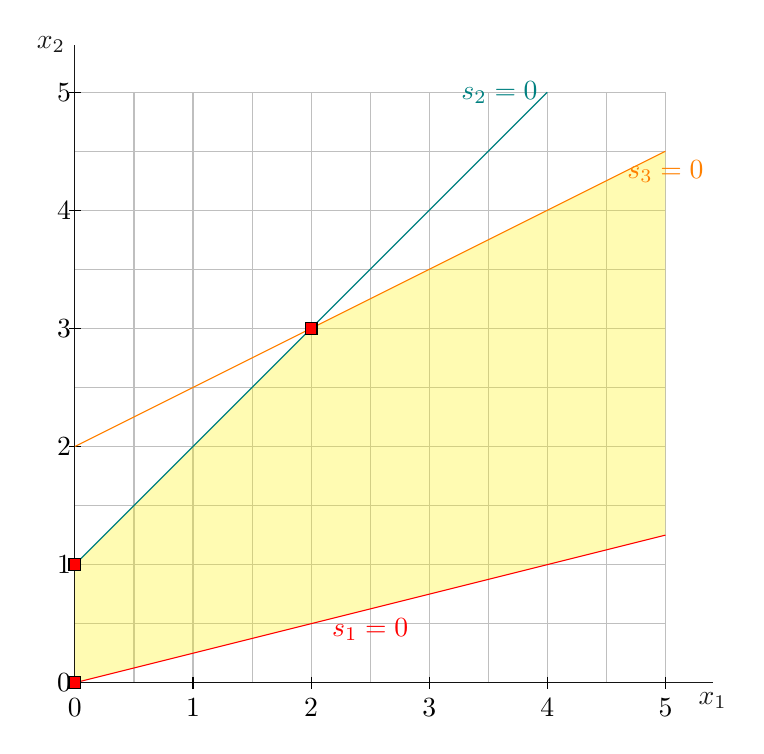
\begin{tikzpicture} [scale=1.5]
    \draw[gray!50, thin, step=.5] (0,0) grid (5,5);
    \draw[opacity=0.9] (0,0) -- (5.4,0) node[below] {$x_1$};
    \draw[opacity=0.9] (0,0) -- (0,5.4) node[left] {$x_2$}; % option \draw[very thick,->]

    \foreach \x in {0,...,5} \draw (\x,0.05) -- (\x,-0.05) node[below] {\x};
    \foreach \y in {0,...,5} \draw (-0.05,\y) -- (0.05,\y) node[left] {\y};

    \fill[yellow,opacity=0.3] (0,0) -- (0,1) -- (2,3) -- (5,4.5) --(5,1.25)-- cycle;

    \draw [red](0,0) -- node[below] {$s_1=0$} (5, 1.25);
    \draw [teal] (0,1)  --  (4,5) node[left, sloped] {$s_2=0$};
    \draw [orange](0,2) --  (5,4.5) node[below, sloped] {$s_3=0$}; %node[above right ,sloped] 
	\filldraw[fill=red] (-0.05,-0.05) rectangle (0.05,0.05);
	\filldraw[fill=red] (-0.05,.95) rectangle (0.05,1.05);
	\filldraw[fill=red] (1.95,2.95) rectangle (2.05,3.05);
\end{tikzpicture} \end{center} 
\end{minipage}

\begin{center}  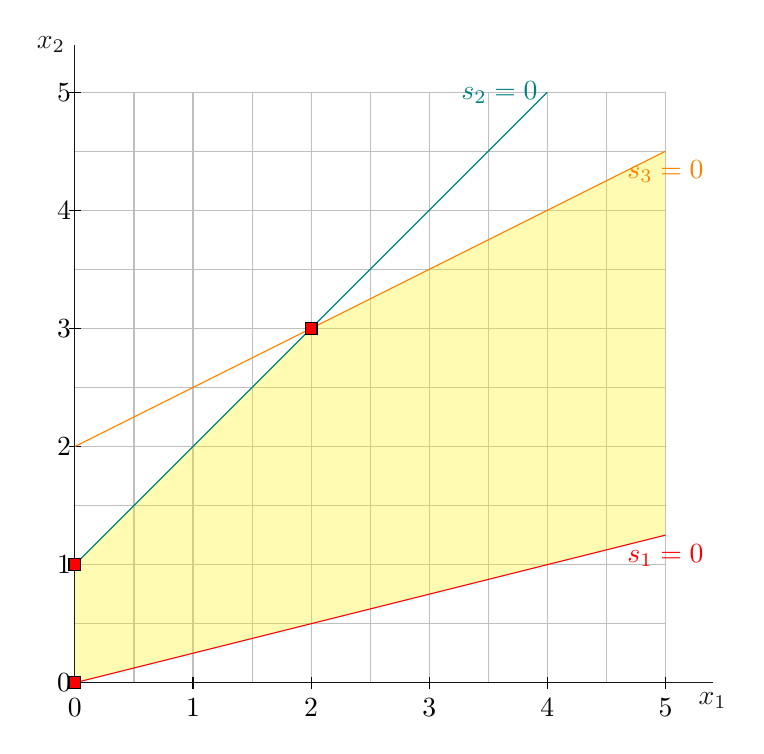
\begin{tikzpicture} [scale=1.5]
    \draw[gray!50, thin, step=.5] (0,0) grid (5,5);
    \draw[opacity=0.9] (0,0) -- (5.4,0) node[below] {$x_1$};
    \draw[opacity=0.9] (0,0) -- (0,5.4) node[left] {$x_2$}; % option \draw[very thick,->]

    \foreach \x in {0,...,5} \draw (\x,0.05) -- (\x,-0.05) node[below] {\x};
    \foreach \y in {0,...,5} \draw (-0.05,\y) -- (0.05,\y) node[left] {\y};

    \fill[yellow,opacity=0.3] (0,0) -- (0,1) -- (2,3) -- (5,4.5) --(5,1.25)-- cycle;

\draw[domain=0:4,smooth,variable=\x, teal] plot ({\x},{\x+1}) node[left] {$s_2=0$};
\draw[domain=0:5,smooth,variable=\x, red] plot ({\x},{\x*1/4}) node[below] {$s_1=0$};
%    \draw [red](0,0) -- node[below] {$s_1=0$} (5, 1.25);
    %\draw [teal] (0,1)  --  (4,5) node[left, sloped] {$s_2=0$};
    \draw [orange](0,2) --  (5,4.5) node[below, sloped] {$s_3=0$}; %node[above right ,sloped] 
	\filldraw[fill=red] (-0.05,-0.05) rectangle (0.05,0.05);
	\filldraw[fill=red] (-0.05,.95) rectangle (0.05,1.05);
	\filldraw[fill=red] (1.95,2.95) rectangle (2.05,3.05);
\end{tikzpicture} \end{center} 

% \draw[scale=0.5,domain=-3:3,smooth,variable=\x,blue] plot ({\x},{\x*\x});


  
\medskip E.g., consider the $s_3=0$ (orange) line, to find the extreme direction start at extreme point (2,3) and find another feasible point on the orange line, say (4,4) and subtract (2,3) from (4,4), which yields (2,1). 

\medskip This is related to the slope in two-dimensions, as discussed in class, the rise is 1 and the run is 2. So this direction has a slope of 1/2, but this does not carry over easily to higher dimensions where directions cannot be defined by a single number. 

\medskip To find the extreme directions we can change the right-hand-side to $\mathbf{b} = \mathbf{0}$, which forms a polyhedral cone (in yellow), and then add the constraint $x_1 + x_2 = 1$. The intersection of the cone and  $x_1 + x_2 = 1$ form a line segment.

\begin{minipage}[t][][b]{.4\linewidth} \vspace{0mm}
\begin{align*}
\mbox{max~~} & z = -5x_1 - x_2  \\
\mbox{s.t.~~} & x_1 - 4x_2 +s_1 = 0  \\
& -x_1 + x_2 + s_2 = 0 \\
& -x_1 + 2x_2 +s_3 = 0 \\
& x_1 + x_2 = 1 \\
& x_1, x_2, s_1, s_2, s_3 \ge 0.
\end{align*}
\end{minipage}%
\begin{minipage}[t][][b]{.6\linewidth}
\begin{center} 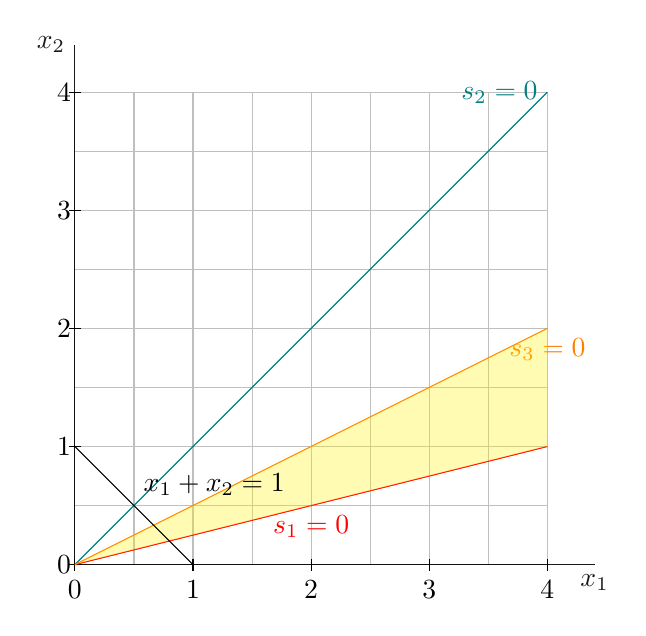
\begin{tikzpicture} [scale=1.5]
\draw[gray!50, thin, step=.5] (0,0) grid (4,4);
\draw[opacity=0.9] (0,0) -- (4.4,0) node[below] {$x_1$};
\draw[opacity=0.9] (0,0) -- (0,4.4) node[left] {$x_2$}; % option \draw[very thick,->]

\foreach \x in {0,...,4} \draw (\x,0.05) -- (\x,-0.05) node[below] {\x};
\foreach \y in {0,...,4} \draw (-0.05,\y) -- (0.05,\y) node[left] {\y};
        
\draw [red](0, 0) -- node[below] {$s_1=0$} (4, 1);
\draw [teal] (0,0)  -- (4,4) node[left, sloped] {$s_2=0$};
\draw [orange](0,0) -- (4,2) node[below, sloped] {$s_3=0$}; 
\fill[yellow,opacity=0.3] (0,0) -- (4,2) -- (4,1) --  cycle; % \draw [orange!50!blue] 

\draw [black] (0,1)  -- node[above right] {$x_1+x_2 = 1$} (1,0); 
\end{tikzpicture} \end{center} 
\end{minipage}



\begin{center} 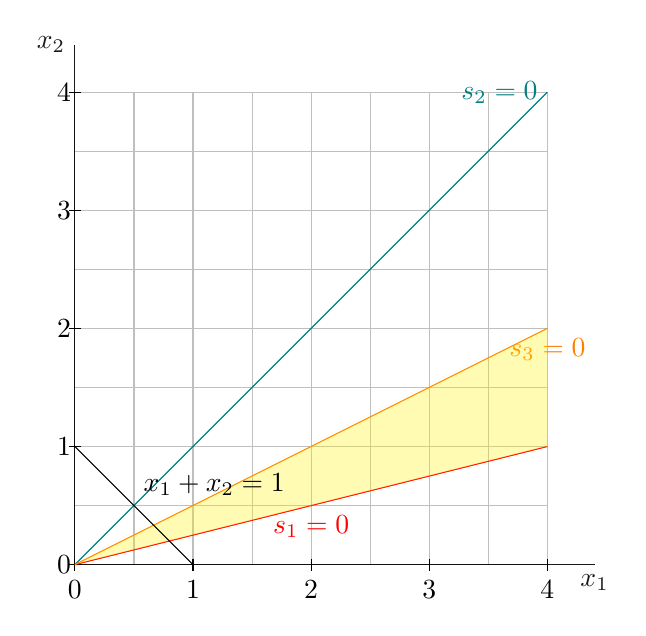
\begin{tikzpicture} [scale=1.5]
\draw[gray!50, thin, step=.5] (0,0) grid (4,4);
\draw[opacity=0.9] (0,0) -- (4.4,0) node[below] {$x_1$};
\draw[opacity=0.9] (0,0) -- (0,4.4) node[left] {$x_2$}; % option \draw[very thick,->]

\foreach \x in {0,...,4} \draw (\x,0.05) -- (\x,-0.05) node[below] {\x};
\foreach \y in {0,...,4} \draw (-0.05,\y) -- (0.05,\y) node[left] {\y};
        
\draw [red](0, 0) -- node[below] {$s_1=0$} (4, 1);
\draw [teal] (0,0)  -- (4,4) node[left, sloped] {$s_2=0$};
\draw [orange](0,0) -- (4,2) node[below, sloped] {$s_3=0$}; 
\fill[yellow,opacity=0.3] (0,0) -- (4,2) -- (4,1) --  cycle; % \draw [orange!50!blue] 

\draw [black] (0,1)  -- node[above right] {$x_1+x_2 = 1$} (1,0); 
\end{tikzpicture} \end{center} 


\medskip Magnifying for clarity, and removing the $s_2=0$ (teal) line, as it is redundant, and marking the extreme points of the new feasible region, (4/5, 1/5) and (2/3, 1/3), with red boxes, we have:

\begin{center}  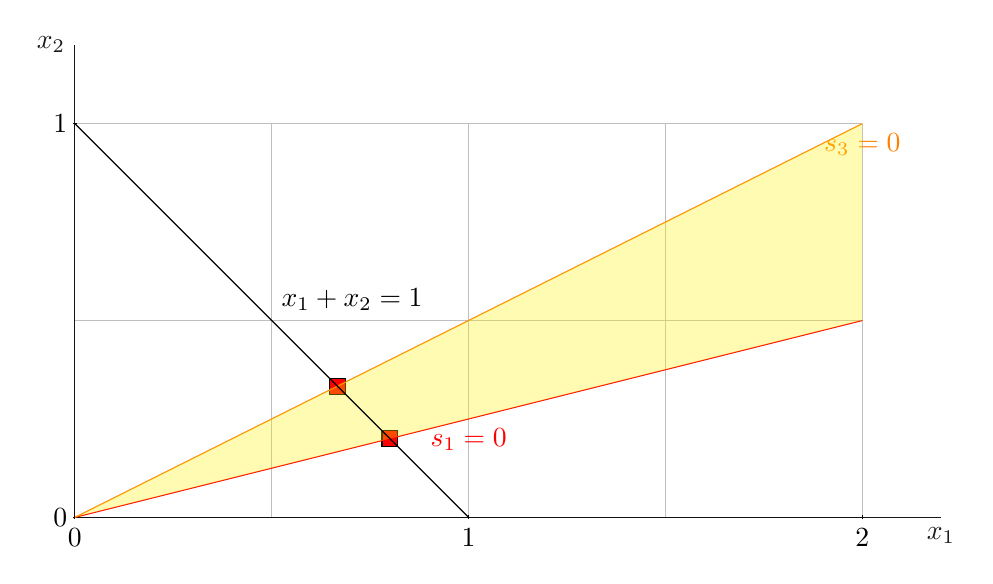
\begin{tikzpicture} [x=50mm, y=50mm] [scale=1.5]
\draw[gray!50, thin, step=.5] (0,0) grid (2,1);
\draw[opacity=0.9] (0,0) -- (2.2,0) node[below] {$x_1$};
\draw[opacity=0.9] (0,0) -- (0,1.2) node[left] {$x_2$}; % option \draw[very thick,->]

\foreach \x in {0,...,2} \draw (\x,0.005) -- (\x,-0.005) node[below] {\x};
\foreach \y in {0,...,1} \draw (-0.005,\y) -- (0.005,\y) node[left] {\y};

\filldraw[fill=red] (0.8-0.02,0.2-0.02) rectangle (0.8+0.02,0.2+0.02);
\filldraw[fill=red] (0.667-0.02,0.333-0.02) rectangle (0.667+0.02,0.333+0.02);

\draw [red](0, 0) -- node[below] {$s_1=0$} (2, .5);
\draw [orange](0,0) -- (2,1) node[below, sloped] {$s_3=0$}; 
\fill[yellow,opacity=0.3] (0,0) -- (2,.5) -- (2,1) --  cycle; % \draw [orange!50!blue] 
\draw [black] (0,1)  -- node[above right] {$x_1+x_2 = 1$} (1,0); 
\end{tikzpicture} \end{center} 

The extreme directions are thus (4/5, 1/5) and (2/3, 1/3). \\

{\bf Representation Theorem:} Let  $\mathbf{x_1}, \mathbf{x_2},\cdots \mathbf{x_k}$ be the set of extreme points of $\mathcal{S}$, and if $\mathcal{S}$ is unbounded, $\mathbf{d_1}, \mathbf{d_2},\cdots \mathbf{d_l}$ be the set of extreme directions. Then any $\mathbf{x} \in \mathcal{S}$ is equal to a convex combination of the extreme points and a non-negative linear combination of the extreme directions: $\mathbf{x} = \sum_{j=1}^k \lambda_j \mathbf{x_j} + \sum_{j=1}^l \mu_j \mathbf{d_j}$, where $\sum_{j=1}^k \lambda_j = 1$, $\lambda_j \ge 0,~\forall  j=1,2,\cdots,k$, and $\mu_j \ge 0,~\forall j=1,2,\cdots,l$.

 \begin{minipage}[t][][b]{.4\linewidth}
\begin{align*}
\mbox{max~~} & z = -5x_1 - x_2  \\\
\mbox{s.t.~~} & x_1 - 4x_2 +s_1 = 0  \\
& -x_1 + x_2 + s_2 = 1 \\
& -x_1 + 2x_2 +s_3 = 4 \\
& x_1, x_2, s_1, s_2, s_3 \ge 0.
\end{align*}
\end{minipage}%
\begin{minipage}[t][][b]{.6\linewidth}
\begin{center}  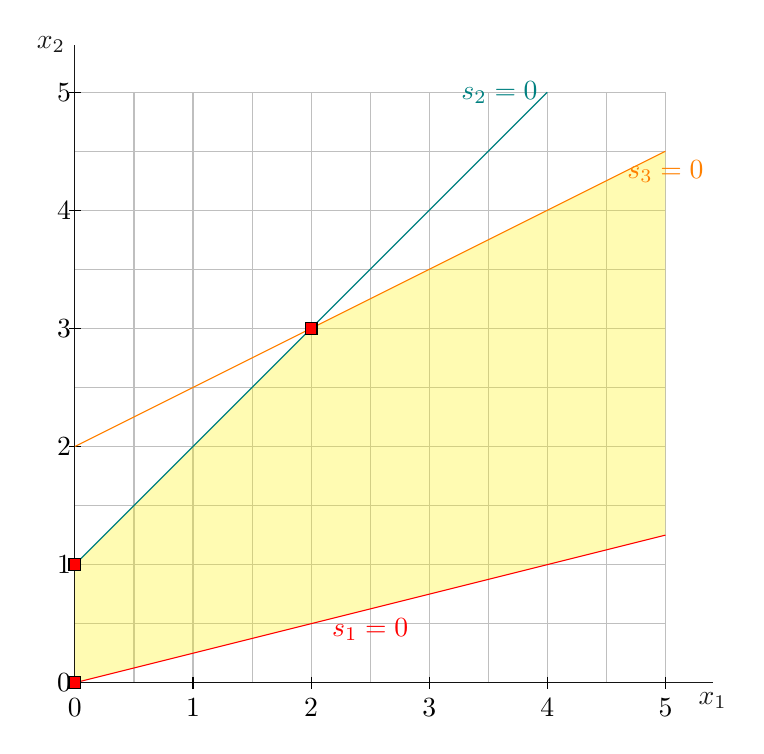
\begin{tikzpicture} [scale=1.5]
    \draw[gray!50, thin, step=.5] (0,0) grid (5,5);
    \draw[opacity=0.9] (0,0) -- (5.4,0) node[below] {$x_1$};
    \draw[opacity=0.9] (0,0) -- (0,5.4) node[left] {$x_2$}; % option \draw[very thick,->]

    \foreach \x in {0,...,5} \draw (\x,0.05) -- (\x,-0.05) node[below] {\x};
    \foreach \y in {0,...,5} \draw (-0.05,\y) -- (0.05,\y) node[left] {\y};

    \fill[yellow,opacity=0.3] (0,0) -- (0,1) -- (2,3) -- (5,4.5) --(5,1.25)-- cycle;

    \draw [red](0,0) -- node[below] {$s_1=0$} (5, 1.25);
    \draw [teal] (0,1)  --  (4,5) node[left, sloped] {$s_2=0$};
    \draw [orange](0,2) --  (5,4.5) node[below, sloped] {$s_3=0$}; %node[above right ,sloped] 
	\filldraw[fill=red] (-0.05,-0.05) rectangle (0.05,0.05);
	\filldraw[fill=red] (-0.05,.95) rectangle (0.05,1.05);
	\filldraw[fill=red] (1.95,2.95) rectangle (2.05,3.05);
\end{tikzpicture} \end{center} 
\end{minipage}




Represent point (1/2, 1) as a convex combination of the extreme points of the above LP.  Find $\lambda$s to solve the following system of equations:

$$\lambda_1 \left[
  \begin{array}{c}
  0 \\
  0 \\
  \end{array} \right]+
 \lambda_2 \left[
  \begin{array}{c}
  0 \\
  1 \\
  \end{array} \right] +
 \lambda_3 \left[
  \begin{array}{c}
  2 \\
  3 \\
  \end{array} \right]  =
 \left[
  \begin{array}{c}
  1/2 \\
  1 \\
  \end{array} \right] 
$$


\newpage The Variable (Canonical Form) and Requirement Space 

\begin{minipage}[t][][b]{.4\linewidth}
\begin{align*}
\mbox{max~~} & z = 2x_1 + x_2  \\\
\mbox{s.t.~~} & x_1 - x_2 +s_1 =  2  \\
& x_1 + x_2 +s_2  = 3 \\
& x_1, x_2, s_1 , s_2  \ge 0.
\end{align*}
\end{minipage}%
\begin{minipage}[t][][b]{.6\linewidth}
\begin{center}  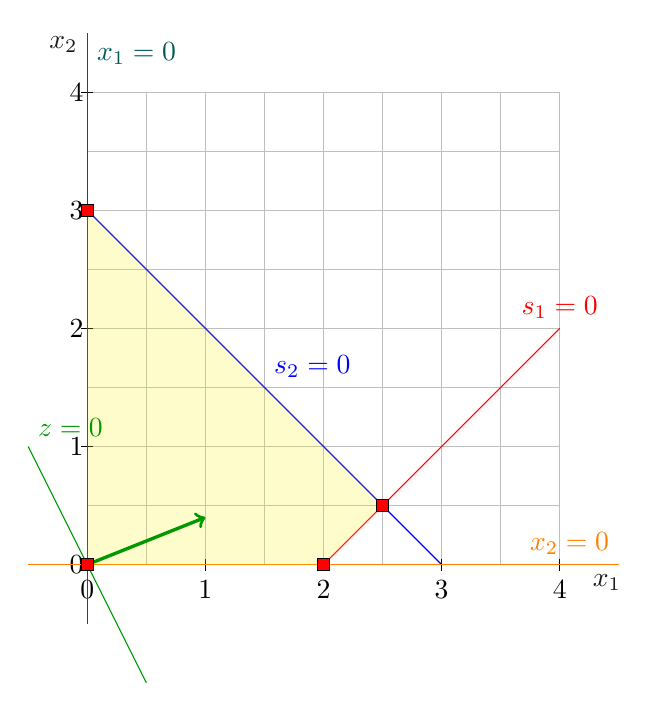
\begin{tikzpicture} [scale=1.5]
\draw[gray!50, thin, step=.5] (0,0) grid (4,4);
\draw[opacity=0.9] (0,0) -- (4.4,0) node[below] {$x_1$};
\draw[opacity=0.9] (0,0) -- (0,4.4) node[left] {$x_2$};

\foreach \x in {0,...,4} \draw (\x,0.05) -- (\x,-0.05) node[below] {\x};
\foreach \y in {0,...,4} \draw (-0.05,\y) -- (0.05,\y) node[left] {\y};

\draw [red](2, 0) --  (4, 2) node[above] {$s_1= 0$};
\draw [blue] (0,3)  -- node[above right] {$s_2=0$} (3,0) ;
\draw [teal!70!black](0,-.5) --  (0,4.5) node[below right] {$x_1=0$}; 
\draw [orange](-.5,0) --  (4.5,0) node[above left] {$x_2=0$}; 

\fill[yellow,opacity=0.2] (0,0) -- (2,0) -- (2.5,0.5) -- (0,3) -- cycle;

\draw [green!60!black] (-0.5, 1)  node[above right] {$z=0$} --  (0.5, -1)  ; % o.f.
\draw [green!60!black, very thick,->](0,0) -- (0+1, 0+2/5); % gradient

\filldraw[fill=red] (-0.05,-0.05) rectangle (0.05,0.05);
\filldraw[fill=red] (2.45,0.45) rectangle (2.55,0.55);
\filldraw[fill=red] (1.95,-0.05) rectangle (2.05,0.05);
\filldraw[fill=red] (-0.05,2.95) rectangle (0.05,3.05);    
\end{tikzpicture} \end{center} 
\end{minipage}



\begin{minipage}[t][][b]{.4\linewidth}
\begin{align*}
\mbox{max~~} & z = 2x_1 + x_2  \\\
\mbox{s.t.~~} & x_1 - x_2 +s_1 =  2  \\
& x_1 + x_2 +s_2  = 3 \\
& x_1, x_2, s_1 , s_2  \ge 0.
\end{align*}
\end{minipage}%
\begin{minipage}[t][][b]{.6\linewidth}
\begin{center}  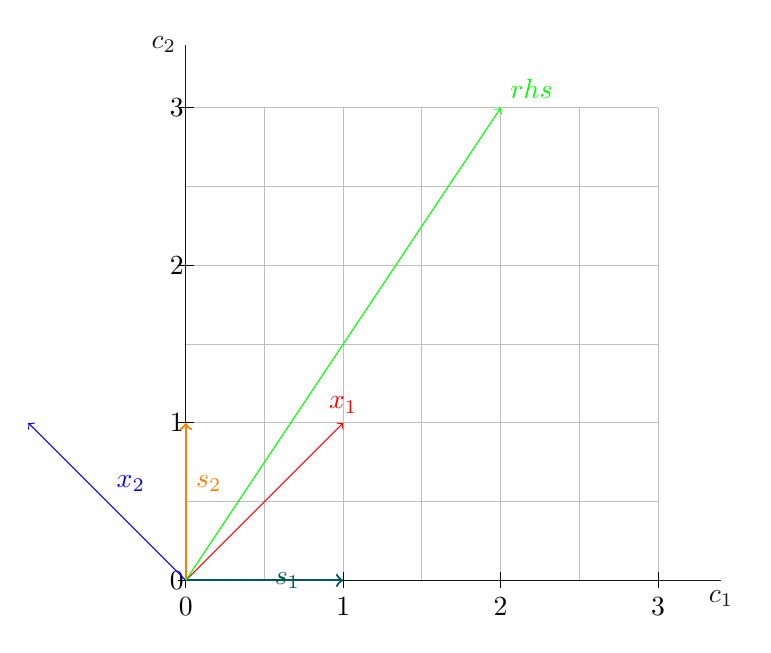
\begin{tikzpicture}[x=20mm, y=20mm] [scale=1.5]  % requirement space
\draw[gray!50, thin, step=.5] (0,0) grid (3,3);
\draw[opacity=0.9] (0,0) -- (3.4,0) node[below] {$c_1$};
\draw[opacity=0.9] (0,0) -- (0,3.4) node[left] {$c_2$};

\foreach \x in {0,...,3} \draw (\x,0.05) -- (\x,-0.05) node[below] {\x};
\foreach \y in {0,...,3} \draw (-0.05,\y) -- (0.05,\y) node[left] {\y};

\draw [red,->](0, 0) --  (1, 1) node[above] {$x_1$};
\draw [blue,->] (0,0)  -- node[above right] {$x_2$} (-1,1) ;
\draw [thick, teal!70!black,->](0,0) -- node[right] {$s_1$} (1,0); 
\draw [thick, orange,->](0,0) -- node[above right] {$s_2$} (0,1); 
\draw [green,->] (0, 0)  --  (2,3) node[above right] {$rhs$}   ; 
\end{tikzpicture} \end{center} 
\end{minipage}





%\section{Graphical Example}
%By Kevin Cheung
%The book is licensed under the
%\href{http://creativecommons.org/licenses/by-sa/4.0/}{Creative Commons
%Attribution-ShareAlike 4.0 International License}.
%
%This file has been modified by Robert Hildebrand 2020.  
%CC BY SA 4.0 licence still applies.

\section{Graphical example}\label{graphic}

To motivate the subject of linear programming (LP), we begin with a
planning problem that can be solved graphically.

Say you are a vendor of lemonade and lemon juice. Each unit of lemonade
requires 1 lemon and 2 litres of water. Each unit of lemon juice
requires 3 lemons and 1 litre of water. Each unit of lemonade gives a
profit of three dollars. Each unit of lemon juice gives a profit of two
dollars. You have 6 lemons and 4 litres of water available. How many
units of lemonade and lemon juice should you make to maximize profit?

If we let \(x\) denote the number of units of lemonade to be made and
let \(y\) denote the number of units of lemon juice to be made, then the
profit is given by \(3x + 2y\) dollars. We call \(3x + 2y\) the
objective function. Note that there are a number of constraints that
\(x\) and \(y\) must satisfied. First of all, \(x\) and \(y\) should be
nonnegative. The number of lemons needed to make \(x\) units of lemonade
and \(y\) units of lemon juice is \(x+3y\) and cannot exceed 6. The
number of litres of water needed to make \(x\) units of lemonade and
\(y\) units of lemon juice is \(2x+y\) and cannot exceed 4. Hence, to
determine the maximum profit, we need to maximize \(3x + 2y\) subject to
\(x\) and \(y\) satisfying the constraints \(x + 3y \leq 6\),
\(2x + y \leq 4\), \(x \geq 0\), and \(y \geq 0.\)

A more compact way to write the problem is as follows:
\[\begin{array}{rrcrll}
\mbox{maximize } & 3x & + & 2y & \\
\mbox{subject to} 
& x & + & 3y & \leq & 6 \\
& 2x & +&  y & \leq & 4 \\
& x &  & & \geq & 0 \\
& & & y & \geq & 0. \\
\end{array}\]

We can solve this maximizationproblem graphically as follows. We first
sketch the set of \(\begin{bmatrix} x\\ y\end{bmatrix}\) satisfying the
constraints, called the feasible region, on the \((x,y)\)-plane. We then
take the objective function \(3x+2y\) and turn it into an equation of a
line \(3x+2y = z\) where \(z\) is a parameter. Note that as the value of
\(z\) increases, the line defined by the equation \(3x+2y=z\) moves in
the direction of the normal vector
\(\begin{bmatrix} 3 \\ 2\end{bmatrix}\). We call this direction the
direction of improvement. Determining the maximum value of the objective
function, called the optimal value, subject to the contraints amounts to
finding the maximum value of \(z\) so that the line defined by the
equation \(3x+2y=z\) still intersects the feasible region.

\begin{center}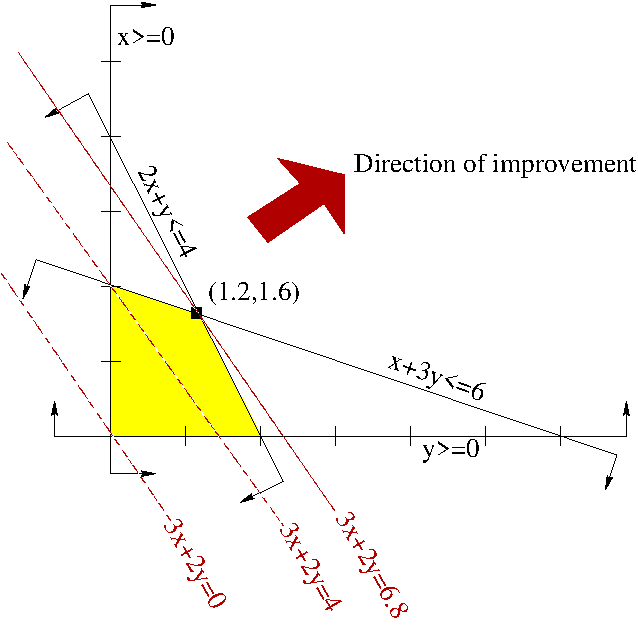
\includegraphics[width=0.8\linewidth]{images/lemon} \end{center}

In the figure above, the lines with \(z\) at 0, 4 and 6.8 have been
drawn. From the picture, we can see that if \(z\) is greater than 6.8,
the line defined by \(3x+2y = z\) will not intersect the feasible
region. Hence, the profit cannot exceed 6.8 dollars.

As the line \(3x+2y = 6.8\) does intersect the feasible region, \(6.8\)
is the maximum value for the objective function. Note that there is only
one point in the feasible region that intersects the line \(3x+2y=6.8\),
namely
\(\begin{bmatrix} x \\ y\end{bmatrix} = \begin{bmatrix} 1.2 \\ 1.6\end{bmatrix}.\)
In other words, to maximize profit, we want to make 1.2 units of
lemonade and 1.6 units of lemon juice.

The above solution method can hardly be regarded as rigorous because we
relied on a picture to conclude that \(3x + 2y \leq 6.8\) for all
\(\begin{bmatrix} x\\y\end{bmatrix}\) satisfying the constraints. But we
can actually show this \emph{algebraically}.

Note that multiplying both sides of the constraint \(x + 3y \leq 6\)
gives \(0.2x + 0.6 y \leq 1.2\), and multiplying both sides of the
constraint \(2x + y \leq 4\) gives \(2.8x + 1.4 y \leq 5.6\). Hence, any
\(\begin{bmatrix} x\\y\end{bmatrix}\) that satisfies both \(x+3y\leq 6\)
and \(2x+y \leq 4\) must also satisfy
\((0.2x+0.6y) + (2.8x+1.4y) \leq 1.2 + 5.6\), which simplifies to
\(3x + 2y \leq 6.8\) as desired! (Here, we used the fact that if
\(a \leq b\) and \(c \leq d\), then \(a+c \leq b+d\).)

Now, one might ask if it is always possible to find an algebraic proof
like the one above for similar problems. If the answer is yes, how does
one find such a proof? We will see answers to this question later on.

Before we end this segment, let us consider the following problem:
\[\begin{array}{rrcrll}
\mbox{minimize } & -2x & + & y & \\
\mbox{subject to} & -x & + & y & \leq & 3 \\
& x & - &  2y & \leq & 2 \\
& x &  & & \geq & 0 \\
& & & y & \geq & 0. \\
\end{array}\]

Note that for any \(t \geq 0\),
\(\begin{bmatrix} x \\ y\end{bmatrix} = \begin{bmatrix} t \\ t\end{bmatrix}\)
satisfies all the constraints. The value of the objective function at
\(\begin{bmatrix} x \\ y\end{bmatrix} = \begin{bmatrix} t \\ t\end{bmatrix}\)
is \(-t\). As \(t \rightarrow \infty\), the value of the objective
function tends to \(-\infty\). Therefore, there is no minimum value for
the objective function. The problem is said to be unbounded. Later on,
we will see how to detect unboundedness algorithmically.

As an exercise, check that unboundedness can also be established by
using
\(\begin{bmatrix} x \\ y\end{bmatrix} = \begin{bmatrix} 2t+2 \\ t\end{bmatrix}\)
for \(t \geq 0\).

\subsection*{Exercises}\label{exercises}
\addcontentsline{toc}{section}{Exercises}

\begin{enumerate}
\def\labelenumi{\arabic{enumi}.}
\item
  Sketch all \(\begin{bmatrix} x \\ y \end{bmatrix}\) satisfying

  \begin{equation*}
  x - 2y \leq 2
  \end{equation*}

  on the \((x,y)\)-plane.
\item
  Determine the optimal value of \[
  \begin{array}{rl}
  \text{Minimize} & x + y \\
  \text{Subject to} &  2x + y \geq 4 \\
  & x + 3y \geq 1.
  \end{array}
  \]
\item
  Show that the problem \[
  \begin{array}{rl}
  \text{Minimize} & -x + y \\
  \text{Subject to} &  2x - y \geq 0 \\
  & x + 3y \geq 3
  \end{array}
  \] is unbounded.
\item
  Suppose that you are shopping for dietary supplements to satisfy your
  required daily intake of 0.40mg of nutrient \(M\) and 0.30mg of
  nutrient \(N\). There are three popular products on the market. The
  costs and the amounts of the two nutrients are given in the following
  table:

  \begin{longtable}[]{@{}lccc@{}}
  \toprule
  & Product 1 & Product 2 & Product 3\tabularnewline
  \midrule
  \endhead
  Cost & \$27 & \$31 & \$24\tabularnewline
  Daily amount of \(M\) & 0.16 mg & 0.21 mg & 0.11 mg\tabularnewline
  Daily amount of \(N\) & 0.19 mg & 0.13 mg & 0.15 mg\tabularnewline
  \bottomrule
  \end{longtable}

  You want to determine how much of each product you should buy so that
  the daily intake requirements of the two nutrients are satisfied at
  minimum cost. Formulate your problem as a linear programming problem,
  assuming that you can buy a fractional number of each product.
\end{enumerate}

\subsection*{Solutions}\label{solutions}
\addcontentsline{toc}{subsection}{Solutions}

\begin{enumerate}
\def\labelenumi{\arabic{enumi}.}
\item
  The points \((x,y)\) satisfying \(x-2y \leq 2\) are precisely those
  above the line passing through \((2,0)\) and \((0,-1)\).
\item
  We want to determine the minimum value \(z\) so that \(x+y=z\) defines
  a line that has a nonempty intersection with the feasible region.
  However, we can avoid referring to a sketch by setting \(x=z-y\) and
  substituting for \(x\) in the inequalities to obtain:

  \begin{eqnarray*}
   2(z-y) + y \geq 4 \\
   (z-y) + 3y \geq 1,
  \end{eqnarray*}

  or equivalently,

  \begin{eqnarray*}
   z \geq 2+\frac{1}{2}y \\
   z \geq 1-2y,
  \end{eqnarray*}

  Thus, the minimum value for \(z\) is
  \(\min \{ 2+\frac{1}{2}y, 1-2y\}\), which occurs at
  \(y = -\frac{2}{5}\). Hence, the optimal value is \(\frac{9}{5}\).

  We can verify our work by doing the following. If our calculations
  above are correct, then an optimal solution is given by
  \(x = \frac{11}{5}\), \(y = -\frac{2}{5}\) since \(x = z - y\). It is
  easy to check that this satisfies both inequalities and therefore is a
  feasible solution.

  Now, taking \(\frac{2}{5}\) times the first inequality and
  \(\frac{1}{5}\) times the second inequality, we can infer the
  inequality \(x+y \geq \frac{9}{5}\). The left-hand side of this
  inequality is precisely the objective function. Hence, no feasible
  solution can have objective function value less than \(\frac{9}{5}\).
  But \(x = \frac{11}{5}\), \(y = -\frac{2}{5}\) is a feasible solution
  with objective function value equal to \(\frac{9}{5}\). As a result,
  it must be an optimal solution.

  \textbf{Remark.} We have not yet discussed how to obtain the
  multipliers \(\frac{2}{5}\) and \(\frac{1}{5}\) for inferring the
  inequality \(x+y \geq \frac{9}{5}\). This is an issue that will be
  taken up later. In the meantime, think about how one could have
  obtained these multipliers for this particular exercise.
\item
  We could glean some insight by first making a sketch on the
  \((x,y)\)-plane.

  The line defined by \(-x + y = z\) has \(x\)-intercept \(-z\). Note
  that for \(z \leq -3\),
  \(\begin{bmatrix} x\\y \end{bmatrix} = \begin{bmatrix} -z\\ 0\end{bmatrix}\)
  satisfies both inequalities and the value of the objective function at
  \(\begin{bmatrix} x\\y \end{bmatrix} = \begin{bmatrix} -z\\ 0\end{bmatrix}\)
  is \(z\). Hence, there is no lower bound on the value of objective
  function.
\item
  Let \(x_i\) denote the amount of Product \(i\) to buy for
  \(i = 1,2,3\). Then, the problem can be formulated as
  \[\begin{array}{rrcrcrll}
  \mbox{minimize } & 27 x_1 & + & 31 x_2 & + & 24 x_3 \\
  \mbox{subject to} 
  & 0.16 x_1 & + & 0.21 x_2 & + & 0.11 x_3 & \geq & 0.30 \\
  & 0.19 x_1 & + & 0.13 x_2 & + & 0.15 x_3 & \geq & 0.40 \\
  & x_1 & , & x_2 & , & x_3 & \geq & 0. \\
  \end{array}\]

  \textbf{Remark.} If one cannot buy fractional amounts of the products,
  the problem can be formulated as \[\begin{array}{rrcrcrll}
  \mbox{minimize } & 27 x_1 & + & 31 x_2 & + & 24 x_3 \\
  \mbox{subject to} 
  & 0.16 x_1 & + & 0.21 x_2 & + & 0.11 x_3 & \geq & 0.30 \\
  & 0.19 x_1 & + & 0.13 x_2 & + & 0.15 x_3 & \geq & 0.40 \\
  & x_1 & , & x_2 & , & x_3 & \geq & 0. \\
  & x_1 & , & x_2 & , & x_3 & \in & \mathbb{Z}. \\
  \end{array}\]
\end{enumerate}


\chapter{CASE STUDY - Designing a campground - Simplex method}
\todoChapter{ 0\% complete. \\
Notes: Borrowed from Karin Vorwerk.  Need to integrate this into other chapters.}
\section{DESIGNING A CAMPGROUND - SIMPLEX METHOD}
The Simplex method is probably the classic method of solving constraint optimization problems. We will use this solution approach, sometimes in modified form, over and over in this class, not just in this chapter.

\begin{outcome}
You will learn

\begin{itemize}
  \item How to recognize linear programming (LP) problems

  \item Vocabulary of LP problems

  \item Graphical solution

  \item Algebraic solution

  \item Excel solution with the Excel Solver

\end{itemize}
\end{outcome}
\subsection{Case Study Description - Campground}
You are opening a campground in the Florida Keys, and you are trying to make as much money as possible. You are planning a mix of RV sites, tent sites, and yurts. Let's assume you already own 10 acres, and that you can make $\$ 80 /$ day profit on each $\mathrm{RV}, \$ 20 /$ day profit on each tent, and $\$ 200$ profit on each Yurt. However, there are restrictions:

\begin{enumerate}
  \item Infrastructure takes up $20 \%$ of your site

  \item You can have 20 RVs per acre, or

  \item You can have 40 tents per acre, or

  \item You can have 10 yurts per acre

  \item You have a budget of $\$ 100,000$. It costs you $\$ 1000$ to develop an $R V$ site, $\$ 200$ for a tent site, and $\$ 8000$ for a yurt.

  \item Maintenance for the bath houses etc. is $15 \mathrm{~min} /$ week/camper unit. You can afford 70hrs/week in maintenance help

  \item Zoning ordinance requires you to have at least 20 tent sites What is the best layout for your campground, and how much profit can you make per day?

\end{enumerate}
\subsection{References}
This case study was inspired by the Knights Key RV park in Florida. Read more about it here: \href{http://www.knightskeyrvresortandmarina.com/news/}{http://www.knightskeyrvresortandmarina.com/news/} \href{http://www.miaminewtimes.com/news/developers-plan-to-replace-rv-park-with-fivestar-resort-stirs-fears-hopes-in-keys-8038648}{http://www.miaminewtimes.com/news/developers-plan-to-replace-rv-park-with-fivestar-resort-stirs-fears-hopes-in-keys-8038648}

\subsection{Solution Approach - Two Variables}
We will again first look at a simpler problem by ignoring the yurts and only considering RV spaces and tents.

Let $r$ be the number of RVs, $t$ the number of tents, and $P(r, t)$ the profit. Your goal is to maximize $P(r, t)=$ $80 \mathrm{r}+20 \mathrm{t}$. This function is called the objective function. The variables $r$ and $t$ are called decision

variables. You can see that in the current case $P(r, t)$ gets bigger if you increase $r$ and/or $t$. If you picture a graph with $r$ on the horizontal and $t$ on the vertical axis, then the direction of increase for the objective function is to the top right.

Translating the relevant restrictions into equations gives

\begin{enumerate}
  \item $r / 20+t / 40 \leq 8$

  \item $r \leq 160$

  \item $t \leq 320$

  \item $(r+t) / 4 \leq 70$

  \item $t \geq 20$

  \item $r, t \geq 0$

  \item $1,000 r+200 t \leq 100,000$

\end{enumerate}
Simplified

\begin{enumerate}
  \item $2 r+t \leq 320$

  \item $r \leq 160$

  \item $t \leq 320$

  \item $5 r+t \leq 500$

  \item $r+t \leq 280$

  \item $\mathrm{t} \geq 20$

  \item $r, t \geq 0$

\end{enumerate}
These are called the functional constraints.

In addition, you can't have negative sites, so we have the non-negativity constraints

\begin{enumerate}
  \setcounter{enumi}{5}
  \item $r \geq 0$

  \item $t \geq 0$.

\end{enumerate}
A problem like the above with linear constraints and a linear objective function is called a linear programming problem.

\subsection{Assumptions made about linear programming problem}
\paragraph{Proportionality} For both the objective function and the constraints, a change in a decision variable will result in a proportional change in the objective function or constraint. (Note that this rules out any exponents on the decision variables other than 1.)

\paragraph{Additivity} Both the objective function and the constraints are the sums of the respective changes in the decision variables (This means no multiplying different decision variables).

Basically, the proportionality and additivity assumptions are just fancy ways of saying that all functions in a linear programming problem are linear in the decision variables.

\paragraph{Divisibility} We are assuming that our decision variables can be non-integer, i.e. may take on fractional values. Problems with an integer constraint are called integer programming problems, we will only touch on them briefly later. Certainty We act as if the value assigned to each parameter is known, precise, and constant over time. This is rarely the case, so we need to compensate for that by performing sensitivity analysis. Basically, we need to investigate how much it affects our solution if the parameters change.

\subsection{Graphical Simplex solution procedure}
We will start with some vocabulary:

\begin{itemize}
  \item Feasible solution: A solution for which all constraints are satisfied, not necessarily an optimal Solution.

  \item Infeasible solution: A solution that violates at least one constraint.

  \item Optimal solution: a solution that optimizes (could be a minimum or maximum, depending on your problem) the objective function. There may or may not be an optimal solution.

\end{itemize}
Feasible region: The set of all feasible solutions

\begin{itemize}
  \item Corner point: the intersection of two or more constraints

  \item Corner point feasible solution CPF solution: A solution that occurs at a corner of the feasible region

\end{itemize}
The first step in the graphical solution procedure is to draw the feasible region (note that this gets really ugly if you have three or more variables).

The non-negativity constraints mean that we are looking for a solution in the first quadrant only. The constraints 2) $r \leq 160,3) t \leq 320$, and 7) $t \geq 20$ mean you have to stay left of the line $r=160$, below the line $t=320$ and above the line $t=20$. You see that the constraint $t \geq 20$ dominates the constraint $t \geq 0$, so the latter is redundant.

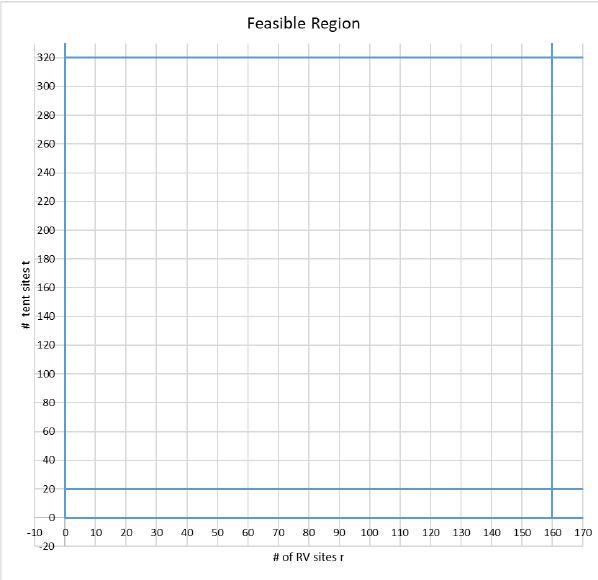
\includegraphics[scale = 0.35]{2022_07_05_5945264bba2a5f6ba667g-28}

Adding the remaining constraints yields this graph: Go ahead, shade the feasible region and identify all redundant constraints.

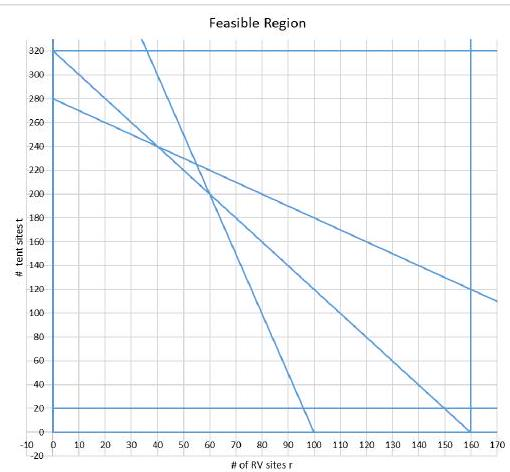
\includegraphics[scale = 0.5]{2022_07_05_5945264bba2a5f6ba667g-29}

All the points in the feasible region are possible solutions. Your job is to pick (one of) the best solutions. Note that there may not be a single best solution but rather several optimal solutions.

We have not yet used the objective function $P(r, t)=80 r+20 t$. Because we do not have a value for $P(r, t)$, so we will draw $P(r, t)$ for a few random values of $P(r, t)$ to get an idea of what it looks like. For $P(r, t)=1600,2400,3200$ we get the lines shown in the next picture. Note that they are all parallel, and that the lines corresponding to the larger value of $P(r, t)$ move to the top left. The direction of increase is just as we expected, to the top right.

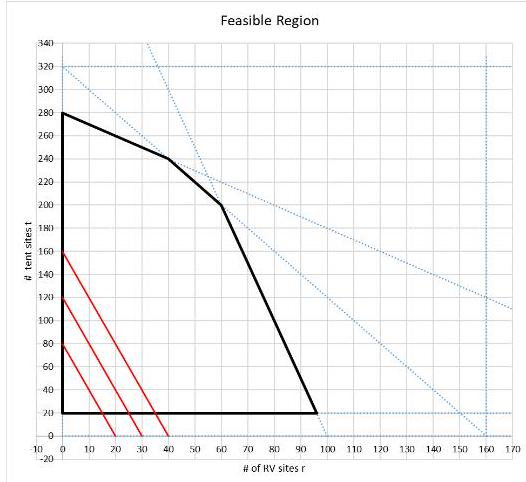
\includegraphics[scale = 0.5]{2022_07_05_5945264bba2a5f6ba667g-29(1)}

As you move the line for the $P(r, t)$ to the right you increase your profit. But you also have to stay in the feasible region. Convince yourself that one of two cases will occur: either a unique optimal solution will be found at a corner point, or infinitely many optimal solutions returning the same maximum value for $P(r, t)$ will be found along a section of the boundary of the feasible region that includes two corner points. Therefore, we need to compute the corner points, i.e. the intersections of the constraints, and move $P(r, t)$ as far to the right as possible without leaving the feasible region.

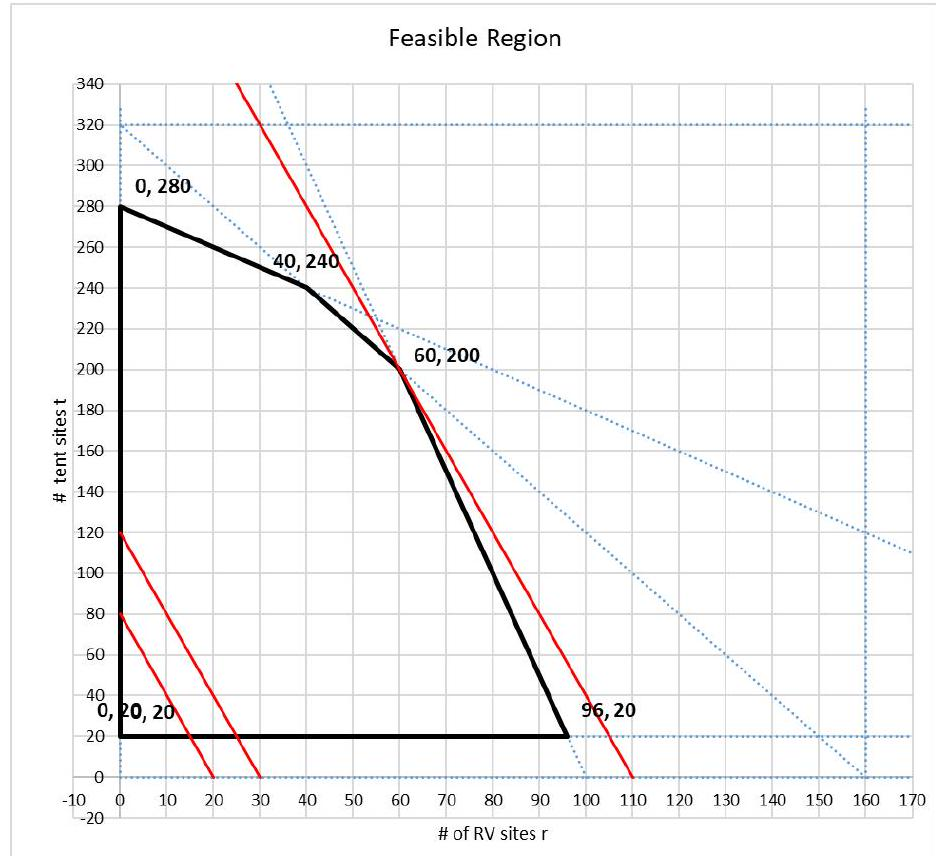
\includegraphics[scale = 0.3]{2022_07_05_5945264bba2a5f6ba667g-30}

From the picture above, you can see that the optimal solution will be at the intersection of the lines corresponding to constraints 1) and 5).
$$
r / 20+t / 40 \leq 8 \text { and } 1000 t+200 t \leq 100,000
$$
which is at the point $r=60, t=200$. (Now would be a good time to review how to solve systems of equations....). This gives us a profit $P(60,200)=60 \cdot \$ 80+200 \cdot \$ 20=\$ 8800$.

\subsection{Stating the Solution}
In OR, typically someone hires you to work your problem, and then expects you to give the answer in the context of the problem. You can't just say "the solution is at $r=60, t=200, P(r, t)=8800$ ". Give the answer like this:

"To maximize potential profit, the campground should have $60 \mathrm{RV}$ sites and 200 tent sites. In that case, the potential profit per day, assuming full occupancy, is $\$ 8800$. You are limited by the available land and budget available, not by available labor or any zoning rules. You will have to hire 65 hours of help per week (260 camping units at 15 minutes/week/unit)."

\subsection{Refinements to the graphical solution}
One "brute force" approach to the graphical solution method would be to compute all intersections of all constraints, check if that corner is in the feasible region, and then compute the objective function at those points. However, the number of intersections increases quadratically with the number of lines ( $\frac{\mathrm{n}(\mathrm{n}+1)}{2}$ for $n$ non-parallel lines), so this approach quickly gets out of hand. Instead, the idea is to start at an easy to find corner of the feasible region. Often, the origin works. From that point, check the adjacent feasible corner points and move to the "best". Continue until there is no more improvement. Here is what that would look like in our case:

We start at a simple corner. Usually, people use the origin, which is not on the feasible region here, so we start at $(0,20)$. Adjacent corners are $(0,280)$ and $(96,20)$ with $P(0,20)=400, P(0,280)=5600$, and $P(96,20)=8080$. $(96,20)$ is best, so we move there. Next, check the adjacent corner $(60,200)$. It gives $P(60,200)=8800$ which is an improvement, so move there. Check the next adjacent corner $(40,240)$ It gives $P(40,240)=8000$. This is worse, so $(60,200)$ is the optimal solution.\\

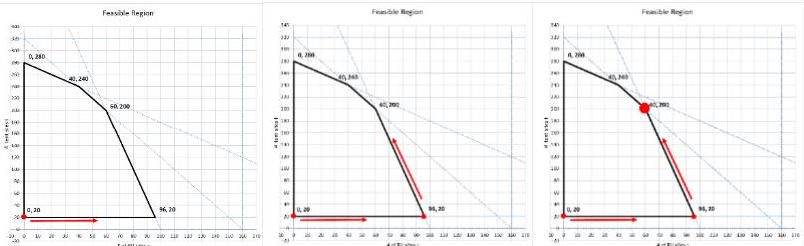
\includegraphics[scale = 0.5]{2022_07_05_5945264bba2a5f6ba667g-31}

There is of course a big problem with this approach. It relies on us having a graph of the feasible region and being able to see the adjacent feasible corner points. If you are dealing with a large number of constraints and variables, this is not possible. We therefor take the idea of looking at adjacent feasible corners and moving towards the one that gives the best value for the objective function, and translate it into an algebraic method.

\paragraph{Solution Approach - Algebraic Simplex Method}
As these are only three variables, we could still draw the feasible region, now a solid bound by planes. However, we need an approach that works for any number of variables. The key to this method is the fact that an optimal solution will occur at a corner point of the feasible region. While the n-dimensional proof is beyond the scope of this class, this fact should be intuitively clear in the 2-d and 3-d cases.

We will first demonstrate the algebraic method on the two-variable problem (RV and tent only) and then solve the full problem.

\paragraph{Corner points, interior corner points, slack variables}
We introduce slack variables to turn the inequalities into equalities. Basically, a slack variable lets you know how close you are to maxing out the constraint. In the current case, we have:

\begin{tabular}{ll}
Constraints &
Augmented constraints\\
1) $4 r+t \leq 320$ &
1) $2 r+t+s_{1}=320$\\
2) $5 r+t \leq 500$&
2) $5 r+t+s_{2}=500$\\
3) $r+t \leq 280$&
3) $r+t+s_{3}=280$\\
4) $t \geq 20$&
4) $\mathrm{t}-\mathrm{s}_{4}=20$\\
5) $r, t \geq 0$&
5) $r, t, s_{1}, s_{2}, s_{3}, s_{4} \geq 0$
\end{tabular}

A point is a corner point if it sits at the intersection of two or more constraints, i.e. if two or more slack variables are zero. A point is a feasible solution (i.e. inside the feasible region) if all slack variables are non-negative. A point is outside the feasible region if any slack variable is negative. We will from now on express each point as $\left(r, t, s_{1}, s_{2}, s_{3}, s_{4}\right)$. Given $r$ and $t$, one computes the values of the slack variables from the augmented constraints.

$\begin{array}{lllll}\text { Examples: } & r=100, t=20 \quad \rightarrow \quad(100,20,100,-20,140,0) & \text { outside the feasible region } \\ & r=10, t=30 \quad & \rightarrow & (10,30,270,420,240,10) & \text { inside feasible region } \\ r=150, t=20 & \rightarrow & (150,20,0,-270,110,0) & \text { corner outside feasible region }\end{array}$

\paragraph{Initializing}
Because $(0,0)$ is not on the feasible region, we again start at $(r, t)=(0,20)$, which has the augmented form $(0,20,300,480,240,0)$. We are sitting on the intersection of the lines $r=0$ and $t=20$.

\paragraph{The adjusted objective function}
Note: If the origin is a feasible corner point and you start at the origin, you can skip this step.

We are sitting on the intersection of the lines $r=0$ and $t=20$. To reach the next adjacent corner, we have to move along one of those lines, but which one? If we move along the line $r=0$, we move away from the line $t=20$, which is the same as saying we are increasing the corresponding slack, $s_{4}$. If we move along the line $t=20$, we increase $r$. We want to choose the direction of increase that gives us the fastest increase in $P$. The original objective function is $P(r, t)=80 r+20 t$, which does not let us see what happens if we increase $s_{4}$ We have to rewrite $P(r, t)$ in terms of $r$ and $s_{4}$.

Using equation 4) we get $t=20+s_{4}$, and thus $P\left(r, s_{4}\right)=80 r+20\left(20+s_{4}\right)=400+80 r+20 s_{4}$

\subsection*{Determining which way to move}
We want to choose the direction of increase that gives us the fastest increase in P. The objective function is $P\left(r, s_{4}\right)=400+80 r+20 s_{4}$. Because the variable $r$ has the biggest coefficient, 80 , an increase in r should give the best return.

\subsection*{Determining how far to move - the next corner}
We will leave $s_{4}$ at is current value, 0 , and increase $r$ as much as possible without leaving the feasible region, i.e. without having $t, s_{1}, s_{2}, s_{3}, s_{4}$ become negative.

\begin{enumerate}
  \item $2 r+t+s_{1}=320$\\
$s_{1}=320-20-2 r \geq 0$, so $r \leq 150$\\
$s_{2}=500-20-5 r \geq 0$, so $r \leq 96$
  \item $5 r+t+s_{2}=500$\\
$S_{3}=280-20-r \geq 0$, so $r \leq 240$
  \item $r+t+s_{3}=280$
  \item $t-S_{4}=20$\\
$t=20$
\end{enumerate}
So, $r$ can be increased to 96 .

\subsection*{Augmented form of the next corner}
Using $r=96, s_{4}=0$, and substituting into the equations $1-4$, we have the augmented point $(96,20,108,0$, $164,0)$. Note that this is the same corner $(96,20)$ we used above.

\subsection*{The adjusted objective function}
We are now sitting on the intersection of the lines $5 r+t+s_{2}=500$ and $t=20$. To reach the next adjacent corner, we have to move along one of those lines, which means either increasing $s_{2}$ or $s_{4}$. We have to rewrite $P(r, t)$ in terms of $s_{2}$ and $s_{4}$.

Using equations 2 and 4 , we find that $5 r=500-t-s_{2}$ and $t=20+s_{4}$, which yields $5 r=480-s_{4}-s_{2}$. Substituting into $P$ :

$P\left(s_{2}, s_{4}\right)=400+80 r+20 s_{4}=400+16\left(480-s_{4}-s_{2}\right)=20 s_{4}=8080+4 s_{4}-16 s_{2}$

Now we will repeat the above steps until the solution/objective function can no longer be improved upon.

\paragraph{Determining which way to move}
Because the $\mathrm{S}_{4}$ has the only positive coefficient, this is the only direction that will yield an increase in $\mathrm{P}$.

\paragraph{Determining how far to move - the next corner}
We will leave $s_{2}$ at is current value, 0 , and increase $s_{4}$ as much as possible without leaving the feasible region.

\begin{enumerate}
  \item $2 r+t+s_{1}=320 \quad s_{1}=320-t-2 r$
  \item $5 r+t+s_{2}=500$\\
$\mathrm{s}_{2}=500-\mathrm{t}-5 \mathrm{r}$
  \item $r+t+s_{3}=280$\\
$\mathrm{s}_{3}=280-\mathrm{t}-\mathrm{r}$
  \item $t-s_{4}=20$ $\mathrm{t}=20+\mathrm{s}_{4}$
\end{enumerate}
We use that $s_{2}=0$ and $t=20+s_{4}$. This gives the set of equations:

\begin{enumerate}
  \item $s_{1}=108-0.6 s_{4}$\\
$\geq 0$, so $\mathrm{s}_{4} \leq 96$\\
$\geq 0$, so $\mathrm{S}_{4} \leq 480$

  \item $r=96-0.2 s_{4}$\\
$\geq 0$, so $\mathrm{S}_{4} \leq 205$

  \item $\mathrm{s}_{3}=164-0.8 \mathrm{~s}_{4}$

  \item $t=20+s_{4}$

\end{enumerate}
$\geq 0$, so $\mathrm{s}_{4} \geq-20$ (as 20 is positive, this is true anyway) So $\mathrm{S}_{4}$ can be increase up to 180 .

\paragraph{Augmented form of the next corner}
Using $s_{2}=0, s_{4}=180$, and substituting into the equations $1-4$, we have the augmented point $(60,200,0,0$, $20,180)$. Note that this is the second corner $(60,200)$ we used above.

\paragraph{The adjusted objective function}
We again re-write the objective function, this time in terms of $s_{1}$ and $s_{2}$ : $P\left(s_{1}, s_{2}\right)=8080+4 s_{4}-16 s_{2}=8080+4\left(180-1.6 s_{1}\right)-16 s_{2}=8800-6.6 s_{1}-16 s_{2}$. Note that increasing either $s_{1}$ or $s_{2}$ will decrease the value of $P$, so we have reached the maximum. As $s_{1}$ and $s_{2}$ are non-negative, we can also see that the maximum for $P$ occurs when $s_{1}$ and $s_{2}$ are zero, at $P=8800$. Again, this is the same answer we arrived at earlier.

A nice side effect is that we can tell which constraints are holding us back, namely those associated with the zero slack variables $s_{1}$ and $s_{2} . s_{1}$ corresponds to the space limitations, and $s_{2}$ to the budget restrictions.

\subsection*{Solving the full problem}
We are now ready to look at the original problem. We will assume you went to the bank and got a loan for $\$ 246,000$ to supplement your original budget. Here are the constraints again:

\begin{enumerate}
  \item Infrastructure takes up $20 \%$ of your site

  \item You can have $20 \mathrm{RV}$ s per acre, or

  \item You can have 40 tents per acre, or

  \item You can have 10 yurts per acre

  \item You have a budget of $\$ 346,000$. It costs you $\$ 1000$ to develop an RV site, $\$ 200$ for a tent site, and $\$ 8000$ for a yurt.

  \item Maintenance for the bath houses etc. is $15 \mathrm{~min} /$ week/camper unit, you can afford $70 \mathrm{hrs} /$ week in maintenance help

  \item Zoning ordinance requires you to have at least 20 tent sites

\end{enumerate}
\begin{tabular}{|l|l|l|}
\hline
Functional Constraints & $\underline{\text { Simplified Constraints }}$ & $\underline{\text { Augmented Constraints }}$ \\
\hline
$\mathrm{r} / 20+\mathrm{t} / 40+\mathrm{y} / 10 \leq 8$ & $2 \mathrm{r}+\mathrm{t}+4 \mathrm{y} \leq 320$ & $2 \mathrm{r}+\mathrm{t}+4 \mathrm{y}+\mathrm{s}_{1}=320$ \\
$1000 \mathrm{r}+200 \mathrm{t}+8000 \mathrm{y} \leq 346,000$ & $5 r+t+40 \mathrm{y} \leq 1730$ & $5 \mathrm{r}+\mathrm{t}+40 \mathrm{y}+\mathrm{s}_{2}=1750$ \\
$(\mathrm{r}+\mathrm{t}+\mathrm{y}) / 4 \leq 70$ & $\mathrm{r}+\mathrm{t}+\mathrm{y} \leq 280$ & $\mathrm{r}+\mathrm{t}+\mathrm{y}+\mathrm{s}_{3}=280$ \\
$\mathrm{t} \geq 20$ & $\mathrm{t} \geq 20$ & $\mathrm{t}-\mathrm{s}_{4}=20$ \\
\hline
\end{tabular}

\paragraph{Non-negativity constraints:}
$r, t, y_{1}, s_{1}, s_{2}, s_{3}, s_{4} \geq 0$

\paragraph{Objective function:}
Maximize $P(r, t, y)=80 r+20 t+200 y$

\paragraph{Initializing}
Because $(0,0,0)$ is not on the feasible region, we start at $(r, t, y)=(0,20,0)$, which has the augmented form $(0,20,0,300,480,240,0)$. We are sitting on the intersection of the planes $r=0, t=20, y=0$. The augmented form of this corner is $(0,20,0,300,1710,260,0)$

\paragraph{The adjusted objective function}
Rewriting $P$ as $P\left(r, y, s_{4}\right)$ gives: $P\left(P\left(r, y, s_{4}\right)=400+80 r+200 y+20 s_{4}\right.$

\paragraph{Determining which way to move}
Looking at the coefficients of $r, y, s_{4}$ in the objective function, we find that we should increase $y$ and leave $r$ and $s_{4}=0$

\paragraph{Determining how far to move - the next corner}
Using $r=0$ and $s_{4}=0$, the constraints become

$\begin{array}{lllll}t+4 y+s_{1}=320 & 4 y+s_{1}=300 & s_{1}=300-4 y & \geq 0 & \rightarrow y \leq 75 \\ t+40 y+s_{2}=1750 & 40 y+s_{2}=1730 & s_{2}=1730-40 y & \geq 0 & \rightarrow y \leq 42.75 \\ t+y+s_{3}=280 & y+s_{3}=260 & s_{3}=260-y & \geq 0 & \rightarrow y \leq 260\end{array}$

$t=20$

So, y can be increased up to $42.75$

\paragraph{Augmented form of the next corner}
With $\mathrm{r}=0, \mathrm{~s}_{4}=0$, and $\mathrm{y}=42.75$, we find the new augmented corner to be $(0,20,42.75,129,0,217.25,0)$.

\paragraph{The adjusted objective function}
We need to rewrite the objective function in terms of $r, s_{2}$, and $s_{4}$ :

$P\left(r, s_{2}, s_{4}\right)=8950+55 r+15 s_{4}-5 s_{2}$

The solution is not optimal yet, (there are still positive coefficients in the objective function), so we keep going.

\paragraph{Determining which way to move}
We see that we should increase $r$ and leave $s_{2}$ and $s_{4}=0$.

Determining how far to move - the next corner

With $s_{2}$ and $s_{4}=0$, we have

$\begin{array}{llll}2 r+t+4 y+s_{1}=320 & 2 r+4 y+s_{1}=300 & s_{1}=129-1.5 r \geq 0 & \rightarrow r \leq 86 \\ 5 r+t+40 y=1750 & 5 r+40 y=1730 & 40 y=1710-5 r & \\ r+t+y+s_{3}=280 & r+y+s_{3}=260 & s_{3}=236.25-0.875 r \geq 0 & \rightarrow r \leq 342\end{array}$

$t=20$

So, y can be increased up to 86

\paragraph{Augmented form of the next corner}
With $y=86, s_{2}=2$, and $s_{4}=0$ we find the new augmented corner to be $(86,20,32,0,0,142,0)$

\paragraph{The adjusted objective function}
We need to rewrite the objective function in terms of $s_{1}, s_{2}$, and $s_{4}$ :

$P\left(s_{1}, s_{2}, s_{4}\right)=13680-36 \frac{2}{3} s_{1}-1 \frac{1}{3} s_{2}-18 s_{4}$

Note that now all variables have negative coefficients, so we cannot increase the value of P past 13680. The first, second, and fourth constraints are maxed out; we are limited in our ability to increase the profit by space, money, and zoning restrictions.

\subsection*{ Stating the Solution }
To maximize potential profit, the campground should have 86 RV sites, 20 tent sites, and 32 yurts. This will take an initial investment of $\$ 346,000$. The potential profit per day, assuming full occupancy, is $\$ 13,680$. You are limited by the available land and budget available and the zoning law requiring 20 tent sites. You will have to hire $34.5$ hours of help per week (138 camping units at 15 minutes/week/unit)."

\subsection{Solution Approach - Using Excel}
Now that we know how the solution method works, we can use Excel to do the work for us. First, we must set up the work sheet. One way that works well is shown on the next page. The fields highlighted in green are necessary, the others serve to explain and label what we are doing.

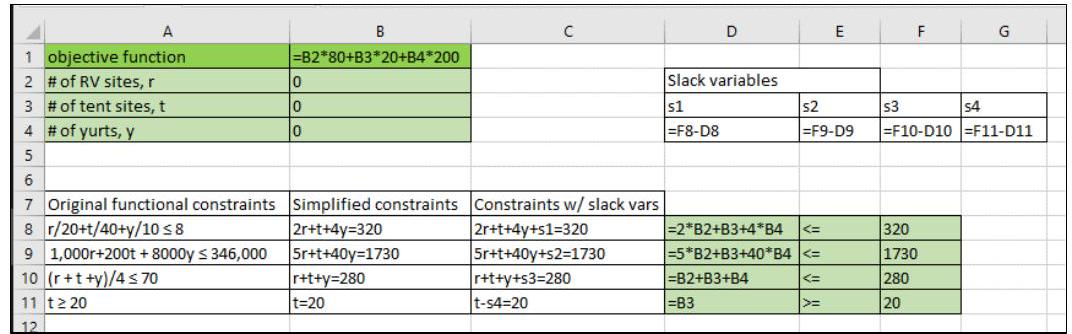
\includegraphics[scale = 0.5]{2022_07_05_5945264bba2a5f6ba667g-37}

Excel has a built-in Solver under the Data tab (if you don't see it, you have to add it in. Go to file/options/Add-ins/Manage Excel Add-ins/Solver Add-in). If you choose "show iteration results in the options tab, the solver will stop at each iteration and show you the corner/solution it has arrived found at that step. You will see that the solver goes through the same steps and corner points as we did when we worked the problem "by hand".

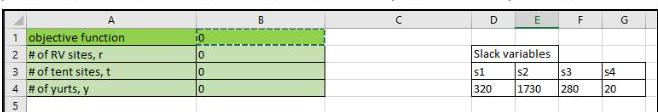
\includegraphics[scale = 0.5]{2022_07_05_5945264bba2a5f6ba667g-37-1}

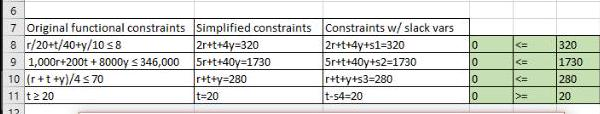
\includegraphics[scale = 0.5]{2022_07_05_5945264bba2a5f6ba667g-37-2}

$All Methods | GRG Nonlinear | Evolutionery |$

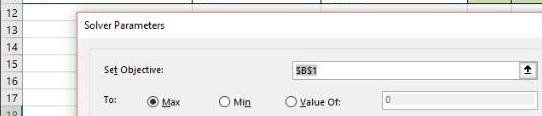
\includegraphics[scale = 0.5]{2022_07_05_5945264bba2a5f6ba667g-37(3)}

Constrainterecisioni. $\quad 0.000001 .$

- Automatic scaling

Whe Automatic scoling

Whow lteration results

Solving with integer Constraints

Solving with integer constraints

\begin{tabular}{l|l|l|}
18 & By Changing Variable Cells: & \$ \\
\hline
19 & SBS2:SBS4 &  \\
20 & Subject to the Constraints: & SDS11 = SFs11 \\
\hline
21 &  &  \\
\hline
\end{tabular}

$\square$ Ignoce integer constraints

By Changing Variable Cells:

$\mathrm{~ - ~ T ~ 2 ~}$

1

(2. $\quad$ Solving Limits

4

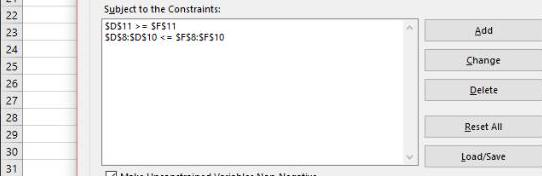
\includegraphics[scale = 0.5]{2022_07_05_5945264bba2a5f6ba667g-37(4)}

Subbject to the Constraints:

Max Iime |Seconds|:

Iterations:

Evolutionary and Integer Constraints:

Evolutionary and inteE

Lox subprobiems:

Mox Ecosible Solutions:

Options


\includegraphics[scale = 0.5]{2022_07_05_5945264bba2a5f6ba667g-37(5)}

\begin{itemize}
  \item 
\end{itemize}
$\square$ Make Unconstrained Variables Non-Negative

Select a Solving\\
Method:

ORtions

Solving Method

Solving Method Select the GRG Nonlinear engine for Solver Problems that are smooth nonlinear. Select the\\
Simplex engine for linear Solver Problems, and select the Evolutionary engine for Solver problems that are non-smooth.

Help

Solve

Close

